
    % latexmk -pdflatex='lualatex' -pdf FontExhibition.tex
    \documentclass[parskip,landscape,letter]{scrartcl}
    \usepackage{fontspec}
    \usepackage[margin=10mm,left=20mm]{geometry}
    \usepackage{tikz}
    \usetikzlibrary{matrix,backgrounds}
    \usepackage{pifont}
    \usepackage{graphicx}
    \usepackage{chessfss}
    \usepackage{setspace}
    \usepackage{enumitem}
    \usepackage{amssymb}
    \usepackage{graphicx,calc}
    \graphicspath{{./graphics/}}
    \usepackage{graphicx,calc}
\newlength\myheight
\newlength\mydepth
\settototalheight\myheight{Xygp}
\settodepth\mydepth{Xygp}
\setlength\fboxsep{0pt}
\newcommand*\inlinegraphics[1]{%
  \settototalheight\myheight{Xygp}%
  \settodepth\mydepth{Xygp}%
  \raisebox{-\mydepth}{\includegraphics[height=\myheight]{#1}}%
}
\providecommand{\Knight}{♘}
\providecommand{\Pawn}{♙}
\providecommand{\King}{♔}
\providecommand{\Queen}{♕}
\providecommand{\Bishop}{♗}
\providecommand{\Rook}{♖}
\providecommand{\KMI}{➊}
% \providecommand{\KII}{➋}
% \providecommand{\KIII}{➌}
% \providecommand{\KIV}{➍} 
\providecommand{\KI}{➀}
\providecommand{\KII}{➁}
\providecommand{\KIII}{➂}
\providecommand{\KIV}{➃}
\providecommand{\Move}{\inlinegraphics{move.png}}
\providecommand{\Attack}{\inlinegraphics{attack.png}}
\providecommand{\Same}{\inlinegraphics{identical.png}}
\providecommand{\Jump}{\inlinegraphics{jump.png}}
\providecommand{\Back}{\inlinegraphics{back.png}}
\providecommand{\Board}{\inlinegraphics{ChessBoard.png}}
\providecommand{\Sym}{\fontsize{20pt}{15pt}\selectfont}
\providecommand{\NoKing}{\inlinegraphics{NOKING.png}}
\providecommand{\NoPawn}{\inlinegraphics{NOPAWN.png}}
\providecommand{\Action}{\inlinegraphics{action.png}}
\providecommand{\PM}{±}
\providecommand{\diff}{⇌}


    \begin{document}
    \setmainfont[Extension={.ttf},ItalicFont={DejaVuSerif-Italic}]{FreeSerif}
    
\begin{tikzpicture}
    \pgfmathsetmacro{\cardroundingradius}{5mm}
    \pgfmathsetmacro{\striproundingradius}{3mm}
    % \pgfmathsetmacro{\cardwidth}{5.9}
    % \pgfmathsetmacro{\cardheight}{9.2}
    \pgfmathsetmacro{\cardwidth}{6.1}  % Magic cards are 63x88mm
    \pgfmathsetmacro{\cardheight}{8.6}
    \pgfmathsetmacro{\stripwidth}{1.2}
    \pgfmathsetmacro{\strippadding}{0.1}
    \pgfmathsetmacro{\textpadding}{0.3}
    \pgfmathsetmacro{\ruleheight}{0.1}
    \providecommand{\stripfontsize}{\Huge}
    \providecommand{\captionfontsize}{\LARGE}
    \providecommand{\textfontsize}{\Large}
    \providecommand{\quotefontsize}{\small}
    \draw[line width=2mm,rounded corners=\cardroundingradius] (0,0) rectangle (\cardwidth,\cardheight);
    \draw[line width=2mm] (0,0) rectangle (\cardwidth,\cardheight);
    \node[text width=(\cardwidth-\strippadding-2*\textpadding)*1cm,below right,inner sep=0] at (\strippadding+\textpadding,\cardheight-\textpadding) 
    { 
    \begin{center} {\fontsize{80pt}{60pt}\selectfont \NoKing}\\\end{center}
\begin{center}
    {\captionfontsize \textsf{\textbf{MOVE SWAP}}}\end{center}
        {\textfontsize Two friendly {\Sym\NoKing} may swap places if one can move to or take the other.}
        \tikz{\fill (0,0) rectangle (\cardwidth-2*\strippadding-2*\textpadding,\ruleheight);}\\
        {\quotefontsize \textit{Trading is very competitive and you have to be able to handle getting your butt kicked. ---Paul Tudor Jones}}\\[-2\baselineskip]
    };
    \node[circle,draw,text=black](c) at (.5,\cardheight-.5){C};
    \node[circle,draw,text=black](c) at (\cardwidth-.5,\cardheight-.5){+};
    \end{tikzpicture}%
\hspace{1pt}%
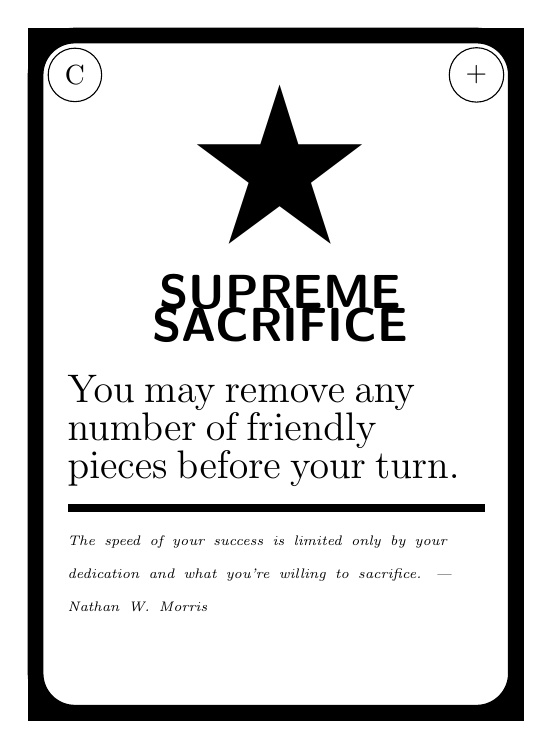
\begin{tikzpicture}
    \pgfmathsetmacro{\cardroundingradius}{5mm}
    \pgfmathsetmacro{\striproundingradius}{3mm}
    % \pgfmathsetmacro{\cardwidth}{5.9}
    % \pgfmathsetmacro{\cardheight}{9.2}
    \pgfmathsetmacro{\cardwidth}{6.1}  % Magic cards are 63x88mm
    \pgfmathsetmacro{\cardheight}{8.6}
    \pgfmathsetmacro{\stripwidth}{1.2}
    \pgfmathsetmacro{\strippadding}{0.1}
    \pgfmathsetmacro{\textpadding}{0.3}
    \pgfmathsetmacro{\ruleheight}{0.1}
    \providecommand{\stripfontsize}{\Huge}
    \providecommand{\captionfontsize}{\LARGE}
    \providecommand{\textfontsize}{\Large}
    \providecommand{\quotefontsize}{\small}
    \draw[line width=2mm,rounded corners=\cardroundingradius] (0,0) rectangle (\cardwidth,\cardheight);
    \draw[line width=2mm] (0,0) rectangle (\cardwidth,\cardheight);
    \node[text width=(\cardwidth-\strippadding-2*\textpadding)*1cm,below right,inner sep=0] at (\strippadding+\textpadding,\cardheight-\textpadding) 
    { 
    \begin{center} {\fontsize{80pt}{60pt}\selectfont \ding{72}}\\\end{center}
\begin{center}
    {\captionfontsize \textsf{\textbf{SUPREME SACRIFICE}}}\end{center}
        {\textfontsize You may remove any number of friendly pieces before your turn.}
        \tikz{\fill (0,0) rectangle (\cardwidth-2*\strippadding-2*\textpadding,\ruleheight);}\\
        {\quotefontsize \textit{\tiny The speed of your success is limited only by your dedication and what you're willing to sacrifice. ---Nathan W. Morris}}\\[-2\baselineskip]
    };
    \node[circle,draw,text=black](c) at (.5,\cardheight-.5){C};
    \node[circle,draw,text=black](c) at (\cardwidth-.5,\cardheight-.5){+};
    \end{tikzpicture}%
\hspace{1pt}%
\begin{tikzpicture}
    \pgfmathsetmacro{\cardroundingradius}{5mm}
    \pgfmathsetmacro{\striproundingradius}{3mm}
    % \pgfmathsetmacro{\cardwidth}{5.9}
    % \pgfmathsetmacro{\cardheight}{9.2}
    \pgfmathsetmacro{\cardwidth}{6.1}  % Magic cards are 63x88mm
    \pgfmathsetmacro{\cardheight}{8.6}
    \pgfmathsetmacro{\stripwidth}{1.2}
    \pgfmathsetmacro{\strippadding}{0.1}
    \pgfmathsetmacro{\textpadding}{0.3}
    \pgfmathsetmacro{\ruleheight}{0.1}
    \providecommand{\stripfontsize}{\Huge}
    \providecommand{\captionfontsize}{\LARGE}
    \providecommand{\textfontsize}{\Large}
    \providecommand{\quotefontsize}{\small}
    \draw[line width=2mm,rounded corners=\cardroundingradius] (0,0) rectangle (\cardwidth,\cardheight);
    \draw[line width=2mm] (0,0) rectangle (\cardwidth,\cardheight);
    \node[text width=(\cardwidth-\strippadding-2*\textpadding)*1cm,below right,inner sep=0] at (\strippadding+\textpadding,\cardheight-\textpadding) 
    { 
    \begin{center} {\fontsize{80pt}{60pt}\selectfont \Board+}\\\end{center}
\begin{center}
    {\captionfontsize \textsf{\textbf{10x8 BOARD}}}\end{center}
        {\textfontsize Add an additional rank on the top and bottom.}
        \tikz{\fill (0,0) rectangle (\cardwidth-2*\strippadding-2*\textpadding,\ruleheight);}\\
        {\quotefontsize \textit{\tiny He who joyfully marches to music in rank and file has already earned my contempt. He has been given a large brain by mistake, since for him the spinal cord would suffice. ---Albert Einstein}}\\[-2\baselineskip]
    };
    \node[circle,draw,text=black](c) at (.5,\cardheight-.5){C};
    \node[circle,draw,text=black](c) at (\cardwidth-.5,\cardheight-.5){+};
    \end{tikzpicture}%
\hspace{1pt}%
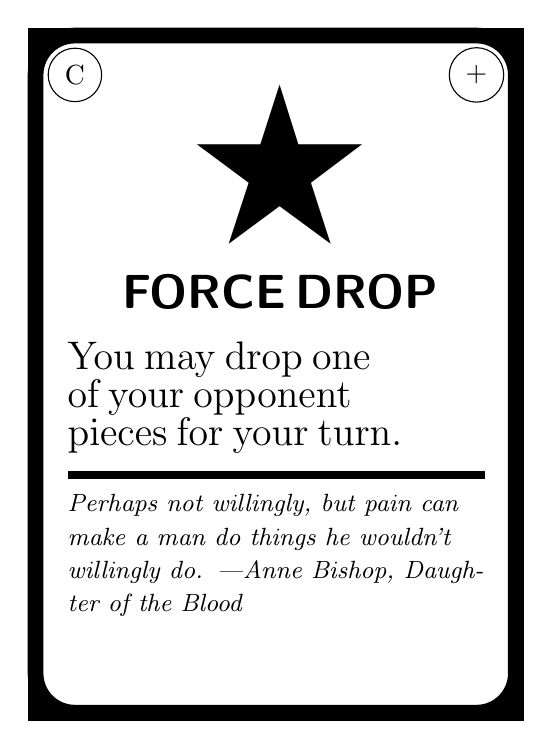
\begin{tikzpicture}
    \pgfmathsetmacro{\cardroundingradius}{5mm}
    \pgfmathsetmacro{\striproundingradius}{3mm}
    % \pgfmathsetmacro{\cardwidth}{5.9}
    % \pgfmathsetmacro{\cardheight}{9.2}
    \pgfmathsetmacro{\cardwidth}{6.1}  % Magic cards are 63x88mm
    \pgfmathsetmacro{\cardheight}{8.6}
    \pgfmathsetmacro{\stripwidth}{1.2}
    \pgfmathsetmacro{\strippadding}{0.1}
    \pgfmathsetmacro{\textpadding}{0.3}
    \pgfmathsetmacro{\ruleheight}{0.1}
    \providecommand{\stripfontsize}{\Huge}
    \providecommand{\captionfontsize}{\LARGE}
    \providecommand{\textfontsize}{\Large}
    \providecommand{\quotefontsize}{\small}
    \draw[line width=2mm,rounded corners=\cardroundingradius] (0,0) rectangle (\cardwidth,\cardheight);
    \draw[line width=2mm] (0,0) rectangle (\cardwidth,\cardheight);
    \node[text width=(\cardwidth-\strippadding-2*\textpadding)*1cm,below right,inner sep=0] at (\strippadding+\textpadding,\cardheight-\textpadding) 
    { 
    \begin{center} {\fontsize{80pt}{60pt}\selectfont \ding{72}}\\\end{center}
\begin{center}
    {\captionfontsize \textsf{\textbf{FORCE DROP}}}\end{center}
        {\textfontsize You may drop one of your opponent pieces for your turn.}
        \tikz{\fill (0,0) rectangle (\cardwidth-2*\strippadding-2*\textpadding,\ruleheight);}\\
        {\quotefontsize \textit{Perhaps not willingly, but pain can make a man do things he wouldn't willingly do. ---Anne Bishop, Daughter of the Blood}}\\[-2\baselineskip]
    };
    \node[circle,draw,text=black](c) at (.5,\cardheight-.5){C};
    \node[circle,draw,text=black](c) at (\cardwidth-.5,\cardheight-.5){+};
    \end{tikzpicture}%
\hspace{1pt}%
\\[-.5\lineskip]
\begin{tikzpicture}
    \pgfmathsetmacro{\cardroundingradius}{5mm}
    \pgfmathsetmacro{\striproundingradius}{3mm}
    % \pgfmathsetmacro{\cardwidth}{5.9}
    % \pgfmathsetmacro{\cardheight}{9.2}
    \pgfmathsetmacro{\cardwidth}{6.1}  % Magic cards are 63x88mm
    \pgfmathsetmacro{\cardheight}{8.6}
    \pgfmathsetmacro{\stripwidth}{1.2}
    \pgfmathsetmacro{\strippadding}{0.1}
    \pgfmathsetmacro{\textpadding}{0.3}
    \pgfmathsetmacro{\ruleheight}{0.1}
    \providecommand{\stripfontsize}{\Huge}
    \providecommand{\captionfontsize}{\LARGE}
    \providecommand{\textfontsize}{\Large}
    \providecommand{\quotefontsize}{\small}
    \draw[line width=2mm,rounded corners=\cardroundingradius] (0,0) rectangle (\cardwidth,\cardheight);
    \draw[line width=2mm] (0,0) rectangle (\cardwidth,\cardheight);
    \node[text width=(\cardwidth-\strippadding-2*\textpadding)*1cm,below right,inner sep=0] at (\strippadding+\textpadding,\cardheight-\textpadding) 
    { 
    \begin{center} {\fontsize{80pt}{60pt}\selectfont \Rook}\\\end{center}
\begin{center}
    {\captionfontsize \textsf{\textbf{SITH v1}}}\end{center}
        {\textfontsize As a premove, your opponent can have one \Rook\ attack the other.}
        \tikz{\fill (0,0) rectangle (\cardwidth-2*\strippadding-2*\textpadding,\ruleheight);}\\
        {\quotefontsize \textit{Always two, there are. No more, no less. A master and an apprentice. ---Yoda}}\\[-2\baselineskip]
    };
    \node[circle,draw,text=black](c) at (.5,\cardheight-.5){C};
    \node[circle,draw,text=black](c) at (\cardwidth-.5,\cardheight-.5){\diff};
    \end{tikzpicture}%
\hspace{1pt}%
\begin{tikzpicture}
    \pgfmathsetmacro{\cardroundingradius}{5mm}
    \pgfmathsetmacro{\striproundingradius}{3mm}
    % \pgfmathsetmacro{\cardwidth}{5.9}
    % \pgfmathsetmacro{\cardheight}{9.2}
    \pgfmathsetmacro{\cardwidth}{6.1}  % Magic cards are 63x88mm
    \pgfmathsetmacro{\cardheight}{8.6}
    \pgfmathsetmacro{\stripwidth}{1.2}
    \pgfmathsetmacro{\strippadding}{0.1}
    \pgfmathsetmacro{\textpadding}{0.3}
    \pgfmathsetmacro{\ruleheight}{0.1}
    \providecommand{\stripfontsize}{\Huge}
    \providecommand{\captionfontsize}{\LARGE}
    \providecommand{\textfontsize}{\Large}
    \providecommand{\quotefontsize}{\small}
    \draw[line width=2mm,rounded corners=\cardroundingradius] (0,0) rectangle (\cardwidth,\cardheight);
    \draw[line width=2mm] (0,0) rectangle (\cardwidth,\cardheight);
    \node[text width=(\cardwidth-\strippadding-2*\textpadding)*1cm,below right,inner sep=0] at (\strippadding+\textpadding,\cardheight-\textpadding) 
    { 
    \begin{center} {\fontsize{80pt}{60pt}\selectfont \Bishop}\\\end{center}
\begin{center}
    {\captionfontsize \textsf{\textbf{SITH v2}}}\end{center}
        {\textfontsize If one \Rook\ is captured, the other is as well. Drop both on the same turn.}
        \tikz{\fill (0,0) rectangle (\cardwidth-2*\strippadding-2*\textpadding,\ruleheight);}\\
        {\quotefontsize \textit{Always two, there are. No more, no less. A master and an apprentice. ---Yoda}}\\[-2\baselineskip]
    };
    \node[circle,draw,text=black](c) at (.5,\cardheight-.5){C};
    \node[circle,draw,text=black](c) at (\cardwidth-.5,\cardheight-.5){\diff};
    \end{tikzpicture}%
\hspace{1pt}%
\begin{tikzpicture}
    \pgfmathsetmacro{\cardroundingradius}{5mm}
    \pgfmathsetmacro{\striproundingradius}{3mm}
    % \pgfmathsetmacro{\cardwidth}{5.9}
    % \pgfmathsetmacro{\cardheight}{9.2}
    \pgfmathsetmacro{\cardwidth}{6.1}  % Magic cards are 63x88mm
    \pgfmathsetmacro{\cardheight}{8.6}
    \pgfmathsetmacro{\stripwidth}{1.2}
    \pgfmathsetmacro{\strippadding}{0.1}
    \pgfmathsetmacro{\textpadding}{0.3}
    \pgfmathsetmacro{\ruleheight}{0.1}
    \providecommand{\stripfontsize}{\Huge}
    \providecommand{\captionfontsize}{\LARGE}
    \providecommand{\textfontsize}{\Large}
    \providecommand{\quotefontsize}{\small}
    \draw[line width=2mm,rounded corners=\cardroundingradius] (0,0) rectangle (\cardwidth,\cardheight);
    \draw[line width=2mm] (0,0) rectangle (\cardwidth,\cardheight);
    \node[text width=(\cardwidth-\strippadding-2*\textpadding)*1cm,below right,inner sep=0] at (\strippadding+\textpadding,\cardheight-\textpadding) 
    { 
    \begin{center} {\fontsize{80pt}{60pt}\selectfont \Queen}\\\end{center}
\begin{center}
    {\captionfontsize \textsf{\textbf{AGENT SMITH}}}\end{center}
        {\textfontsize Your {\Sym\Queen}\ may switch positions with any friendly {\Sym\NoKing}\ piece.}
        \tikz{\fill (0,0) rectangle (\cardwidth-2*\strippadding-2*\textpadding,\ruleheight);}\\
        {\quotefontsize \textit{Me, me, me. ---Agent Smith}}\\[-2\baselineskip]
    };
    \node[circle,draw,text=black](c) at (.5,\cardheight-.5){C};
    \node[circle,draw,text=black](c) at (\cardwidth-.5,\cardheight-.5){+};
    \end{tikzpicture}%
\hspace{1pt}%
\begin{tikzpicture}
    \pgfmathsetmacro{\cardroundingradius}{5mm}
    \pgfmathsetmacro{\striproundingradius}{3mm}
    % \pgfmathsetmacro{\cardwidth}{5.9}
    % \pgfmathsetmacro{\cardheight}{9.2}
    \pgfmathsetmacro{\cardwidth}{6.1}  % Magic cards are 63x88mm
    \pgfmathsetmacro{\cardheight}{8.6}
    \pgfmathsetmacro{\stripwidth}{1.2}
    \pgfmathsetmacro{\strippadding}{0.1}
    \pgfmathsetmacro{\textpadding}{0.3}
    \pgfmathsetmacro{\ruleheight}{0.1}
    \providecommand{\stripfontsize}{\Huge}
    \providecommand{\captionfontsize}{\LARGE}
    \providecommand{\textfontsize}{\Large}
    \providecommand{\quotefontsize}{\small}
    \draw[line width=2mm,rounded corners=\cardroundingradius] (0,0) rectangle (\cardwidth,\cardheight);
    \draw[line width=2mm] (0,0) rectangle (\cardwidth,\cardheight);
    \node[text width=(\cardwidth-\strippadding-2*\textpadding)*1cm,below right,inner sep=0] at (\strippadding+\textpadding,\cardheight-\textpadding) 
    { 
    \begin{center} {\fontsize{80pt}{60pt}\selectfont ☯}\\\end{center}
\begin{center}
    {\captionfontsize \textsf{\textbf{FAIR UNFAIR}}}\end{center}
        {\textfontsize Reveal cards until two matching type cards are found {\Sym(+,-,\diff)}. The first applies to white, the second applies to black.}
        \tikz{\fill (0,0) rectangle (\cardwidth-2*\strippadding-2*\textpadding,\ruleheight);}\\
        {\quotefontsize \textit{I know the world isn't fair, but why isn't it ever unfair in my favor? ---Bill Watterson}}\\[-2\baselineskip]
    };
    \node[circle,draw,text=black](c) at (.5,\cardheight-.5){C};
    \node[circle,draw,text=black](c) at (\cardwidth-.5,\cardheight-.5){?};
    \end{tikzpicture}%
\hspace{1pt}%
\\[-.5\lineskip]
\begin{tikzpicture}
    \pgfmathsetmacro{\cardroundingradius}{5mm}
    \pgfmathsetmacro{\striproundingradius}{3mm}
    % \pgfmathsetmacro{\cardwidth}{5.9}
    % \pgfmathsetmacro{\cardheight}{9.2}
    \pgfmathsetmacro{\cardwidth}{6.1}  % Magic cards are 63x88mm
    \pgfmathsetmacro{\cardheight}{8.6}
    \pgfmathsetmacro{\stripwidth}{1.2}
    \pgfmathsetmacro{\strippadding}{0.1}
    \pgfmathsetmacro{\textpadding}{0.3}
    \pgfmathsetmacro{\ruleheight}{0.1}
    \providecommand{\stripfontsize}{\Huge}
    \providecommand{\captionfontsize}{\LARGE}
    \providecommand{\textfontsize}{\Large}
    \providecommand{\quotefontsize}{\small}
    \draw[line width=2mm,rounded corners=\cardroundingradius] (0,0) rectangle (\cardwidth,\cardheight);
    \draw[line width=2mm] (0,0) rectangle (\cardwidth,\cardheight);
    \node[text width=(\cardwidth-\strippadding-2*\textpadding)*1cm,below right,inner sep=0] at (\strippadding+\textpadding,\cardheight-\textpadding) 
    { 
    \begin{center} {\fontsize{80pt}{60pt}\selectfont \Board}\\\end{center}
\begin{center}
    {\captionfontsize \textsf{\textbf{BOUNCE}}}\end{center}
        {\textfontsize The board continues by reflection in the outer ranks and files.}
        \tikz{\fill (0,0) rectangle (\cardwidth-2*\strippadding-2*\textpadding,\ruleheight);}\\
        {\quotefontsize \textit{Success is how high you bounce when you hit bottom. ---George S. Patton}}\\[-2\baselineskip]
    };
    \node[circle,draw,text=black](c) at (.5,\cardheight-.5){I};
    \node[circle,draw,text=black](c) at (\cardwidth-.5,\cardheight-.5){+};
    \end{tikzpicture}%
\hspace{1pt}%
\begin{tikzpicture}
    \pgfmathsetmacro{\cardroundingradius}{5mm}
    \pgfmathsetmacro{\striproundingradius}{3mm}
    % \pgfmathsetmacro{\cardwidth}{5.9}
    % \pgfmathsetmacro{\cardheight}{9.2}
    \pgfmathsetmacro{\cardwidth}{6.1}  % Magic cards are 63x88mm
    \pgfmathsetmacro{\cardheight}{8.6}
    \pgfmathsetmacro{\stripwidth}{1.2}
    \pgfmathsetmacro{\strippadding}{0.1}
    \pgfmathsetmacro{\textpadding}{0.3}
    \pgfmathsetmacro{\ruleheight}{0.1}
    \providecommand{\stripfontsize}{\Huge}
    \providecommand{\captionfontsize}{\LARGE}
    \providecommand{\textfontsize}{\Large}
    \providecommand{\quotefontsize}{\small}
    \draw[line width=2mm,rounded corners=\cardroundingradius] (0,0) rectangle (\cardwidth,\cardheight);
    \draw[line width=2mm] (0,0) rectangle (\cardwidth,\cardheight);
    \node[text width=(\cardwidth-\strippadding-2*\textpadding)*1cm,below right,inner sep=0] at (\strippadding+\textpadding,\cardheight-\textpadding) 
    { 
    \begin{center} {\fontsize{80pt}{60pt}\selectfont \Board}\\\end{center}
\begin{center}
    {\captionfontsize \textsf{\textbf{CYLINDER}}}\end{center}
        {\textfontsize Pieces may move as if the right and left side of the board are adjacent to each other.}
        \tikz{\fill (0,0) rectangle (\cardwidth-2*\strippadding-2*\textpadding,\ruleheight);}\\
        {\quotefontsize \textit{\tiny Everything in nature takes its form from the sphere, the cone and the cylinder. ---Paul Cezanne}}\\[-2\baselineskip]
    };
    \node[circle,draw,text=black](c) at (.5,\cardheight-.5){I};
    \node[circle,draw,text=black](c) at (\cardwidth-.5,\cardheight-.5){+};
    \end{tikzpicture}%
\hspace{1pt}%
\begin{tikzpicture}
    \pgfmathsetmacro{\cardroundingradius}{5mm}
    \pgfmathsetmacro{\striproundingradius}{3mm}
    % \pgfmathsetmacro{\cardwidth}{5.9}
    % \pgfmathsetmacro{\cardheight}{9.2}
    \pgfmathsetmacro{\cardwidth}{6.1}  % Magic cards are 63x88mm
    \pgfmathsetmacro{\cardheight}{8.6}
    \pgfmathsetmacro{\stripwidth}{1.2}
    \pgfmathsetmacro{\strippadding}{0.1}
    \pgfmathsetmacro{\textpadding}{0.3}
    \pgfmathsetmacro{\ruleheight}{0.1}
    \providecommand{\stripfontsize}{\Huge}
    \providecommand{\captionfontsize}{\LARGE}
    \providecommand{\textfontsize}{\Large}
    \providecommand{\quotefontsize}{\small}
    \draw[line width=2mm,rounded corners=\cardroundingradius] (0,0) rectangle (\cardwidth,\cardheight);
    \draw[line width=2mm] (0,0) rectangle (\cardwidth,\cardheight);
    \node[text width=(\cardwidth-\strippadding-2*\textpadding)*1cm,below right,inner sep=0] at (\strippadding+\textpadding,\cardheight-\textpadding) 
    { 
    \begin{center} {\fontsize{80pt}{60pt}\selectfont \KMI}\\\end{center}
\begin{center}
    {\captionfontsize \textsf{\textbf{CHAMELEON}}}\end{center}
        {\textfontsize {\Sym\KMI\Move: \Same\newline\KMI\Attack:} \KMI\ takes X only as X would take.}
        \tikz{\fill (0,0) rectangle (\cardwidth-2*\strippadding-2*\textpadding,\ruleheight);}\\
        {\quotefontsize \textit{Everybody in life is a chameleon. ---Melanie Chisholm}}\\[-2\baselineskip]
    };
    \node[circle,draw,text=black](c) at (.5,\cardheight-.5){C};
    \node[circle,draw,text=black](c) at (\cardwidth-.5,\cardheight-.5){\diff};
    \end{tikzpicture}%
\hspace{1pt}%
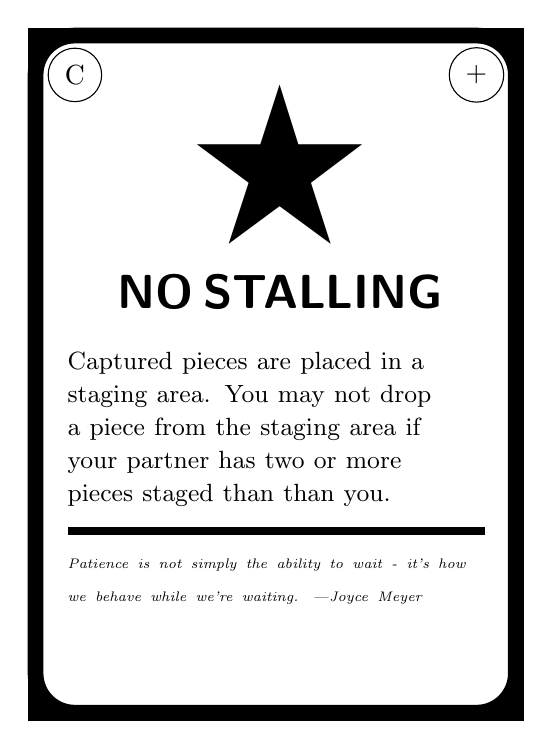
\begin{tikzpicture}
    \pgfmathsetmacro{\cardroundingradius}{5mm}
    \pgfmathsetmacro{\striproundingradius}{3mm}
    % \pgfmathsetmacro{\cardwidth}{5.9}
    % \pgfmathsetmacro{\cardheight}{9.2}
    \pgfmathsetmacro{\cardwidth}{6.1}  % Magic cards are 63x88mm
    \pgfmathsetmacro{\cardheight}{8.6}
    \pgfmathsetmacro{\stripwidth}{1.2}
    \pgfmathsetmacro{\strippadding}{0.1}
    \pgfmathsetmacro{\textpadding}{0.3}
    \pgfmathsetmacro{\ruleheight}{0.1}
    \providecommand{\stripfontsize}{\Huge}
    \providecommand{\captionfontsize}{\LARGE}
    \providecommand{\textfontsize}{\Large}
    \providecommand{\quotefontsize}{\small}
    \draw[line width=2mm,rounded corners=\cardroundingradius] (0,0) rectangle (\cardwidth,\cardheight);
    \draw[line width=2mm] (0,0) rectangle (\cardwidth,\cardheight);
    \node[text width=(\cardwidth-\strippadding-2*\textpadding)*1cm,below right,inner sep=0] at (\strippadding+\textpadding,\cardheight-\textpadding) 
    { 
    \begin{center} {\fontsize{80pt}{60pt}\selectfont \ding{72}}\\\end{center}
\begin{center}
    {\captionfontsize \textsf{\textbf{NO STALLING}}}\end{center}
        {\textfontsize \small Captured pieces are placed in a staging area. You may not drop a piece from the staging area if your partner has two or more pieces staged than than you.}
        \tikz{\fill (0,0) rectangle (\cardwidth-2*\strippadding-2*\textpadding,\ruleheight);}\\
        {\quotefontsize \textit{\tiny Patience is not simply the ability to wait - it's how we behave while we're waiting. ---Joyce Meyer}}\\[-2\baselineskip]
    };
    \node[circle,draw,text=black](c) at (.5,\cardheight-.5){C};
    \node[circle,draw,text=black](c) at (\cardwidth-.5,\cardheight-.5){+};
    \end{tikzpicture}%
\hspace{1pt}%
\\[-.5\lineskip]
\begin{tikzpicture}
    \pgfmathsetmacro{\cardroundingradius}{5mm}
    \pgfmathsetmacro{\striproundingradius}{3mm}
    % \pgfmathsetmacro{\cardwidth}{5.9}
    % \pgfmathsetmacro{\cardheight}{9.2}
    \pgfmathsetmacro{\cardwidth}{6.1}  % Magic cards are 63x88mm
    \pgfmathsetmacro{\cardheight}{8.6}
    \pgfmathsetmacro{\stripwidth}{1.2}
    \pgfmathsetmacro{\strippadding}{0.1}
    \pgfmathsetmacro{\textpadding}{0.3}
    \pgfmathsetmacro{\ruleheight}{0.1}
    \providecommand{\stripfontsize}{\Huge}
    \providecommand{\captionfontsize}{\LARGE}
    \providecommand{\textfontsize}{\Large}
    \providecommand{\quotefontsize}{\small}
    \draw[line width=2mm,rounded corners=\cardroundingradius] (0,0) rectangle (\cardwidth,\cardheight);
    \draw[line width=2mm] (0,0) rectangle (\cardwidth,\cardheight);
    \node[text width=(\cardwidth-\strippadding-2*\textpadding)*1cm,below right,inner sep=0] at (\strippadding+\textpadding,\cardheight-\textpadding) 
    { 
    \begin{center} {\fontsize{80pt}{60pt}\selectfont \Rook}\\\end{center}
\begin{center}
    {\captionfontsize \textsf{\textbf{TWO FACED}}}\end{center}
        {\textfontsize Rooks may invert after an action. Inverted rooks act like bishops.}
        \tikz{\fill (0,0) rectangle (\cardwidth-2*\strippadding-2*\textpadding,\ruleheight);}\\
        {\quotefontsize \textit{God has given you one face, and you make yourself another. ---William Shakespeare}}\\[-2\baselineskip]
    };
    \node[circle,draw,text=black](c) at (.5,\cardheight-.5){C};
    \node[circle,draw,text=black](c) at (\cardwidth-.5,\cardheight-.5){+};
    \end{tikzpicture}%
\hspace{1pt}%
\begin{tikzpicture}
    \pgfmathsetmacro{\cardroundingradius}{5mm}
    \pgfmathsetmacro{\striproundingradius}{3mm}
    % \pgfmathsetmacro{\cardwidth}{5.9}
    % \pgfmathsetmacro{\cardheight}{9.2}
    \pgfmathsetmacro{\cardwidth}{6.1}  % Magic cards are 63x88mm
    \pgfmathsetmacro{\cardheight}{8.6}
    \pgfmathsetmacro{\stripwidth}{1.2}
    \pgfmathsetmacro{\strippadding}{0.1}
    \pgfmathsetmacro{\textpadding}{0.3}
    \pgfmathsetmacro{\ruleheight}{0.1}
    \providecommand{\stripfontsize}{\Huge}
    \providecommand{\captionfontsize}{\LARGE}
    \providecommand{\textfontsize}{\Large}
    \providecommand{\quotefontsize}{\small}
    \draw[line width=2mm,rounded corners=\cardroundingradius] (0,0) rectangle (\cardwidth,\cardheight);
    \draw[line width=2mm] (0,0) rectangle (\cardwidth,\cardheight);
    \node[text width=(\cardwidth-\strippadding-2*\textpadding)*1cm,below right,inner sep=0] at (\strippadding+\textpadding,\cardheight-\textpadding) 
    { 
    \begin{center} {\fontsize{80pt}{60pt}\selectfont \NoKing}\\\end{center}
\begin{center}
    {\captionfontsize \textsf{\textbf{CROWDSURF}}}\end{center}
        {\textfontsize \NoKing${\Action}^+$: Any non-King piece can crowdsurf.}
        \tikz{\fill (0,0) rectangle (\cardwidth-2*\strippadding-2*\textpadding,\ruleheight);}\\
        {\quotefontsize \textit{\tiny The joy of surfing is so many things combined, from the physical exertion of it to the challenge of it, to the mental side of the sport. ---Kelly Slater}}\\[-2\baselineskip]
    };
    \node[circle,draw,text=black](c) at (.5,\cardheight-.5){C};
    \node[circle,draw,text=black](c) at (\cardwidth-.5,\cardheight-.5){+};
    \end{tikzpicture}%
\hspace{1pt}%
\begin{tikzpicture}
    \pgfmathsetmacro{\cardroundingradius}{5mm}
    \pgfmathsetmacro{\striproundingradius}{3mm}
    % \pgfmathsetmacro{\cardwidth}{5.9}
    % \pgfmathsetmacro{\cardheight}{9.2}
    \pgfmathsetmacro{\cardwidth}{6.1}  % Magic cards are 63x88mm
    \pgfmathsetmacro{\cardheight}{8.6}
    \pgfmathsetmacro{\stripwidth}{1.2}
    \pgfmathsetmacro{\strippadding}{0.1}
    \pgfmathsetmacro{\textpadding}{0.3}
    \pgfmathsetmacro{\ruleheight}{0.1}
    \providecommand{\stripfontsize}{\Huge}
    \providecommand{\captionfontsize}{\LARGE}
    \providecommand{\textfontsize}{\Large}
    \providecommand{\quotefontsize}{\small}
    \draw[line width=2mm,rounded corners=\cardroundingradius] (0,0) rectangle (\cardwidth,\cardheight);
    \draw[line width=2mm] (0,0) rectangle (\cardwidth,\cardheight);
    \node[text width=(\cardwidth-\strippadding-2*\textpadding)*1cm,below right,inner sep=0] at (\strippadding+\textpadding,\cardheight-\textpadding) 
    { 
    \begin{center} {\fontsize{80pt}{60pt}\selectfont \NoPawn}\\\end{center}
\begin{center}
    {\captionfontsize \textsf{\textbf{THREE'S A CROWD}}}\end{center}
        {\textfontsize You may not have more that two of any \NoPawn\ on the board, including promoted pieces.}
        \tikz{\fill (0,0) rectangle (\cardwidth-2*\strippadding-2*\textpadding,\ruleheight);}\\
        {\quotefontsize \textit{Every crowd has a silver lining. ---P.T. Barnum}}\\[-2\baselineskip]
    };
    \node[circle,draw,text=black](c) at (.5,\cardheight-.5){C};
    \node[circle,draw,text=black](c) at (\cardwidth-.5,\cardheight-.5){-};
    \end{tikzpicture}%
\hspace{1pt}%
\begin{tikzpicture}
    \pgfmathsetmacro{\cardroundingradius}{5mm}
    \pgfmathsetmacro{\striproundingradius}{3mm}
    % \pgfmathsetmacro{\cardwidth}{5.9}
    % \pgfmathsetmacro{\cardheight}{9.2}
    \pgfmathsetmacro{\cardwidth}{6.1}  % Magic cards are 63x88mm
    \pgfmathsetmacro{\cardheight}{8.6}
    \pgfmathsetmacro{\stripwidth}{1.2}
    \pgfmathsetmacro{\strippadding}{0.1}
    \pgfmathsetmacro{\textpadding}{0.3}
    \pgfmathsetmacro{\ruleheight}{0.1}
    \providecommand{\stripfontsize}{\Huge}
    \providecommand{\captionfontsize}{\LARGE}
    \providecommand{\textfontsize}{\Large}
    \providecommand{\quotefontsize}{\small}
    \draw[line width=2mm,rounded corners=\cardroundingradius] (0,0) rectangle (\cardwidth,\cardheight);
    \draw[line width=2mm] (0,0) rectangle (\cardwidth,\cardheight);
    \node[text width=(\cardwidth-\strippadding-2*\textpadding)*1cm,below right,inner sep=0] at (\strippadding+\textpadding,\cardheight-\textpadding) 
    { 
    \begin{center} {\fontsize{80pt}{60pt}\selectfont \NoKing}\\\end{center}
\begin{center}
    {\captionfontsize \textsf{\textbf{NEAR SWAP}}}\end{center}
        {\textfontsize \NoKing${\Action}^+$: Two adjacent friendly \NoKing\ pieces may swap places.}
        \tikz{\fill (0,0) rectangle (\cardwidth-2*\strippadding-2*\textpadding,\ruleheight);}\\
        {\quotefontsize \textit{\tiny Would I swap what I have achieved as a cook if I could have been as successful as a footballer? Definitely. ---Gordon Ramsay}}\\[-2\baselineskip]
    };
    \node[circle,draw,text=black](c) at (.5,\cardheight-.5){C};
    \node[circle,draw,text=black](c) at (\cardwidth-.5,\cardheight-.5){+};
    \end{tikzpicture}%
\hspace{1pt}%
\\[-.5\lineskip]
\begin{tikzpicture}
    \pgfmathsetmacro{\cardroundingradius}{5mm}
    \pgfmathsetmacro{\striproundingradius}{3mm}
    % \pgfmathsetmacro{\cardwidth}{5.9}
    % \pgfmathsetmacro{\cardheight}{9.2}
    \pgfmathsetmacro{\cardwidth}{6.1}  % Magic cards are 63x88mm
    \pgfmathsetmacro{\cardheight}{8.6}
    \pgfmathsetmacro{\stripwidth}{1.2}
    \pgfmathsetmacro{\strippadding}{0.1}
    \pgfmathsetmacro{\textpadding}{0.3}
    \pgfmathsetmacro{\ruleheight}{0.1}
    \providecommand{\stripfontsize}{\Huge}
    \providecommand{\captionfontsize}{\LARGE}
    \providecommand{\textfontsize}{\Large}
    \providecommand{\quotefontsize}{\small}
    \draw[line width=2mm,rounded corners=\cardroundingradius] (0,0) rectangle (\cardwidth,\cardheight);
    \draw[line width=2mm] (0,0) rectangle (\cardwidth,\cardheight);
    \node[text width=(\cardwidth-\strippadding-2*\textpadding)*1cm,below right,inner sep=0] at (\strippadding+\textpadding,\cardheight-\textpadding) 
    { 
    \begin{center} {\fontsize{80pt}{60pt}\selectfont \NoKing}\\\end{center}
\begin{center}
    {\captionfontsize \textsf{\textbf{KNIGHT SWAP}}}\end{center}
        {\textfontsize \NoKing${\Action}^+$: Two friendly \NoKing\ pieces which are a standard knight move apart may swap places.}
        \tikz{\fill (0,0) rectangle (\cardwidth-2*\strippadding-2*\textpadding,\ruleheight);}\\
        {\quotefontsize \textit{Don't swap horses in crossing a stream. --Abraham Lincoln}}\\[-2\baselineskip]
    };
    \node[circle,draw,text=black](c) at (.5,\cardheight-.5){C};
    \node[circle,draw,text=black](c) at (\cardwidth-.5,\cardheight-.5){+};
    \end{tikzpicture}%
\hspace{1pt}%
\begin{tikzpicture}
    \pgfmathsetmacro{\cardroundingradius}{5mm}
    \pgfmathsetmacro{\striproundingradius}{3mm}
    % \pgfmathsetmacro{\cardwidth}{5.9}
    % \pgfmathsetmacro{\cardheight}{9.2}
    \pgfmathsetmacro{\cardwidth}{6.1}  % Magic cards are 63x88mm
    \pgfmathsetmacro{\cardheight}{8.6}
    \pgfmathsetmacro{\stripwidth}{1.2}
    \pgfmathsetmacro{\strippadding}{0.1}
    \pgfmathsetmacro{\textpadding}{0.3}
    \pgfmathsetmacro{\ruleheight}{0.1}
    \providecommand{\stripfontsize}{\Huge}
    \providecommand{\captionfontsize}{\LARGE}
    \providecommand{\textfontsize}{\Large}
    \providecommand{\quotefontsize}{\small}
    \draw[line width=2mm,rounded corners=\cardroundingradius] (0,0) rectangle (\cardwidth,\cardheight);
    \draw[line width=2mm] (0,0) rectangle (\cardwidth,\cardheight);
    \node[text width=(\cardwidth-\strippadding-2*\textpadding)*1cm,below right,inner sep=0] at (\strippadding+\textpadding,\cardheight-\textpadding) 
    { 
    \begin{center} {\fontsize{80pt}{60pt}\selectfont \KI}\\\end{center}
\begin{center}
    {\captionfontsize \textsf{\textbf{MAJOR X}}}\end{center}
        {\textfontsize \Sym\KI$\Move^+\Attack^+$: \PM[2,2]}
        \tikz{\fill (0,0) rectangle (\cardwidth-2*\strippadding-2*\textpadding,\ruleheight);}\\
        {\quotefontsize \textit{\hspace{1cm}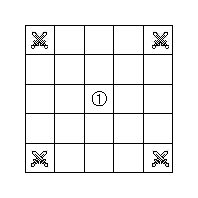
\includegraphics{MAJORX.pdf}}}\\[-2\baselineskip]
    };
    \node[circle,draw,text=black](c) at (.5,\cardheight-.5){C};
    \node[circle,draw,text=black](c) at (\cardwidth-.5,\cardheight-.5){+};
    \end{tikzpicture}%
\hspace{1pt}%
\begin{tikzpicture}
    \pgfmathsetmacro{\cardroundingradius}{5mm}
    \pgfmathsetmacro{\striproundingradius}{3mm}
    % \pgfmathsetmacro{\cardwidth}{5.9}
    % \pgfmathsetmacro{\cardheight}{9.2}
    \pgfmathsetmacro{\cardwidth}{6.1}  % Magic cards are 63x88mm
    \pgfmathsetmacro{\cardheight}{8.6}
    \pgfmathsetmacro{\stripwidth}{1.2}
    \pgfmathsetmacro{\strippadding}{0.1}
    \pgfmathsetmacro{\textpadding}{0.3}
    \pgfmathsetmacro{\ruleheight}{0.1}
    \providecommand{\stripfontsize}{\Huge}
    \providecommand{\captionfontsize}{\LARGE}
    \providecommand{\textfontsize}{\Large}
    \providecommand{\quotefontsize}{\small}
    \draw[line width=2mm,rounded corners=\cardroundingradius] (0,0) rectangle (\cardwidth,\cardheight);
    \draw[line width=2mm] (0,0) rectangle (\cardwidth,\cardheight);
    \node[text width=(\cardwidth-\strippadding-2*\textpadding)*1cm,below right,inner sep=0] at (\strippadding+\textpadding,\cardheight-\textpadding) 
    { 
    \begin{center} {\fontsize{80pt}{60pt}\selectfont \KII}\\\end{center}
\begin{center}
    {\captionfontsize \textsf{\textbf{MINOR +}}}\end{center}
        {\textfontsize \Sym\KII$\Move^+\Attack^+$: \PM[0,1]}
        \tikz{\fill (0,0) rectangle (\cardwidth-2*\strippadding-2*\textpadding,\ruleheight);}\\
        {\quotefontsize \textit{\hspace{1cm}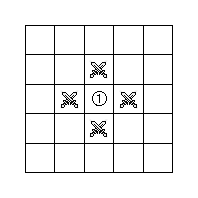
\includegraphics{MINORPLUS.pdf}}}\\[-2\baselineskip]
    };
    \node[circle,draw,text=black](c) at (.5,\cardheight-.5){C};
    \node[circle,draw,text=black](c) at (\cardwidth-.5,\cardheight-.5){+};
    \end{tikzpicture}%
\hspace{1pt}%
\begin{tikzpicture}
    \pgfmathsetmacro{\cardroundingradius}{5mm}
    \pgfmathsetmacro{\striproundingradius}{3mm}
    % \pgfmathsetmacro{\cardwidth}{5.9}
    % \pgfmathsetmacro{\cardheight}{9.2}
    \pgfmathsetmacro{\cardwidth}{6.1}  % Magic cards are 63x88mm
    \pgfmathsetmacro{\cardheight}{8.6}
    \pgfmathsetmacro{\stripwidth}{1.2}
    \pgfmathsetmacro{\strippadding}{0.1}
    \pgfmathsetmacro{\textpadding}{0.3}
    \pgfmathsetmacro{\ruleheight}{0.1}
    \providecommand{\stripfontsize}{\Huge}
    \providecommand{\captionfontsize}{\LARGE}
    \providecommand{\textfontsize}{\Large}
    \providecommand{\quotefontsize}{\small}
    \draw[line width=2mm,rounded corners=\cardroundingradius] (0,0) rectangle (\cardwidth,\cardheight);
    \draw[line width=2mm] (0,0) rectangle (\cardwidth,\cardheight);
    \node[text width=(\cardwidth-\strippadding-2*\textpadding)*1cm,below right,inner sep=0] at (\strippadding+\textpadding,\cardheight-\textpadding) 
    { 
    \begin{center} {\fontsize{80pt}{60pt}\selectfont \KI}\\\end{center}
\begin{center}
    {\captionfontsize \textsf{\textbf{MAJOR +}}}\end{center}
        {\textfontsize \Sym\KI$\Move^+\Attack^+$: \PM[0,2]}
        \tikz{\fill (0,0) rectangle (\cardwidth-2*\strippadding-2*\textpadding,\ruleheight);}\\
        {\quotefontsize \textit{\hspace{1cm}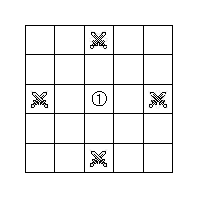
\includegraphics{MAJORPLUS.pdf}}}\\[-2\baselineskip]
    };
    \node[circle,draw,text=black](c) at (.5,\cardheight-.5){C};
    \node[circle,draw,text=black](c) at (\cardwidth-.5,\cardheight-.5){+};
    \end{tikzpicture}%
\hspace{1pt}%
\\[-.5\lineskip]
\begin{tikzpicture}
    \pgfmathsetmacro{\cardroundingradius}{5mm}
    \pgfmathsetmacro{\striproundingradius}{3mm}
    % \pgfmathsetmacro{\cardwidth}{5.9}
    % \pgfmathsetmacro{\cardheight}{9.2}
    \pgfmathsetmacro{\cardwidth}{6.1}  % Magic cards are 63x88mm
    \pgfmathsetmacro{\cardheight}{8.6}
    \pgfmathsetmacro{\stripwidth}{1.2}
    \pgfmathsetmacro{\strippadding}{0.1}
    \pgfmathsetmacro{\textpadding}{0.3}
    \pgfmathsetmacro{\ruleheight}{0.1}
    \providecommand{\stripfontsize}{\Huge}
    \providecommand{\captionfontsize}{\LARGE}
    \providecommand{\textfontsize}{\Large}
    \providecommand{\quotefontsize}{\small}
    \draw[line width=2mm,rounded corners=\cardroundingradius] (0,0) rectangle (\cardwidth,\cardheight);
    \draw[line width=2mm] (0,0) rectangle (\cardwidth,\cardheight);
    \node[text width=(\cardwidth-\strippadding-2*\textpadding)*1cm,below right,inner sep=0] at (\strippadding+\textpadding,\cardheight-\textpadding) 
    { 
    \begin{center} {\fontsize{80pt}{60pt}\selectfont \Board+}\\\end{center}
\begin{center}
    {\captionfontsize \textsf{\textbf{8x10 BOARD}}}\end{center}
        {\textfontsize The legal playing area includes an additional file on the right and left.}
        \tikz{\fill (0,0) rectangle (\cardwidth-2*\strippadding-2*\textpadding,\ruleheight);}\\
        {\quotefontsize \textit{The Bureau doesn't have any secret files. ---W. Mark Felt}}\\[-2\baselineskip]
    };
    \node[circle,draw,text=black](c) at (.5,\cardheight-.5){C};
    \node[circle,draw,text=black](c) at (\cardwidth-.5,\cardheight-.5){+};
    \end{tikzpicture}%
\hspace{1pt}%
\begin{tikzpicture}
    \pgfmathsetmacro{\cardroundingradius}{5mm}
    \pgfmathsetmacro{\striproundingradius}{3mm}
    % \pgfmathsetmacro{\cardwidth}{5.9}
    % \pgfmathsetmacro{\cardheight}{9.2}
    \pgfmathsetmacro{\cardwidth}{6.1}  % Magic cards are 63x88mm
    \pgfmathsetmacro{\cardheight}{8.6}
    \pgfmathsetmacro{\stripwidth}{1.2}
    \pgfmathsetmacro{\strippadding}{0.1}
    \pgfmathsetmacro{\textpadding}{0.3}
    \pgfmathsetmacro{\ruleheight}{0.1}
    \providecommand{\stripfontsize}{\Huge}
    \providecommand{\captionfontsize}{\LARGE}
    \providecommand{\textfontsize}{\Large}
    \providecommand{\quotefontsize}{\small}
    \draw[line width=2mm,rounded corners=\cardroundingradius] (0,0) rectangle (\cardwidth,\cardheight);
    \draw[line width=2mm] (0,0) rectangle (\cardwidth,\cardheight);
    \node[text width=(\cardwidth-\strippadding-2*\textpadding)*1cm,below right,inner sep=0] at (\strippadding+\textpadding,\cardheight-\textpadding) 
    { 
    \begin{center} {\fontsize{80pt}{60pt}\selectfont \Board+}\\\end{center}
\begin{center}
    {\captionfontsize \textsf{\textbf{FLOOR IS LAVA}}}\end{center}
        {\textfontsize Pieces ending their turn on the four central squares die. Pieces may move over lava.}
        \tikz{\fill (0,0) rectangle (\cardwidth-2*\strippadding-2*\textpadding,\ruleheight);}\\
        {\quotefontsize \textit{\tiny Zeal is a volcano, the peak of which the grass of indecisiveness does not grow. ---Khalil Gibran}}\\[-2\baselineskip]
    };
    \node[circle,draw,text=black](c) at (.5,\cardheight-.5){C};
    \node[circle,draw,text=black](c) at (\cardwidth-.5,\cardheight-.5){+};
    \end{tikzpicture}%
\hspace{1pt}%
\begin{tikzpicture}
    \pgfmathsetmacro{\cardroundingradius}{5mm}
    \pgfmathsetmacro{\striproundingradius}{3mm}
    % \pgfmathsetmacro{\cardwidth}{5.9}
    % \pgfmathsetmacro{\cardheight}{9.2}
    \pgfmathsetmacro{\cardwidth}{6.1}  % Magic cards are 63x88mm
    \pgfmathsetmacro{\cardheight}{8.6}
    \pgfmathsetmacro{\stripwidth}{1.2}
    \pgfmathsetmacro{\strippadding}{0.1}
    \pgfmathsetmacro{\textpadding}{0.3}
    \pgfmathsetmacro{\ruleheight}{0.1}
    \providecommand{\stripfontsize}{\Huge}
    \providecommand{\captionfontsize}{\LARGE}
    \providecommand{\textfontsize}{\Large}
    \providecommand{\quotefontsize}{\small}
    \draw[line width=2mm,rounded corners=\cardroundingradius] (0,0) rectangle (\cardwidth,\cardheight);
    \draw[line width=2mm] (0,0) rectangle (\cardwidth,\cardheight);
    \node[text width=(\cardwidth-\strippadding-2*\textpadding)*1cm,below right,inner sep=0] at (\strippadding+\textpadding,\cardheight-\textpadding) 
    { 
    \begin{center} {\fontsize{80pt}{60pt}\selectfont \Rook}\\\end{center}
\begin{center}
    {\captionfontsize \textsf{\textbf{BLOCKADE}}}\end{center}
        {\textfontsize At the end of a Rook action, it may be inverted. Upside-down rooks move normally, but cannot be taken or attack.}
        \tikz{\fill (0,0) rectangle (\cardwidth-2*\strippadding-2*\textpadding,\ruleheight);}\\
        {\quotefontsize \textit{Everyone thinks at some point if what they are doing has any meaning or not. ---William Macbeth}}\\[-2\baselineskip]
    };
    \node[circle,draw,text=black](c) at (.5,\cardheight-.5){C};
    \node[circle,draw,text=black](c) at (\cardwidth-.5,\cardheight-.5){+};
    \end{tikzpicture}%
\hspace{1pt}%
\begin{tikzpicture}
    \pgfmathsetmacro{\cardroundingradius}{5mm}
    \pgfmathsetmacro{\striproundingradius}{3mm}
    % \pgfmathsetmacro{\cardwidth}{5.9}
    % \pgfmathsetmacro{\cardheight}{9.2}
    \pgfmathsetmacro{\cardwidth}{6.1}  % Magic cards are 63x88mm
    \pgfmathsetmacro{\cardheight}{8.6}
    \pgfmathsetmacro{\stripwidth}{1.2}
    \pgfmathsetmacro{\strippadding}{0.1}
    \pgfmathsetmacro{\textpadding}{0.3}
    \pgfmathsetmacro{\ruleheight}{0.1}
    \providecommand{\stripfontsize}{\Huge}
    \providecommand{\captionfontsize}{\LARGE}
    \providecommand{\textfontsize}{\Large}
    \providecommand{\quotefontsize}{\small}
    \draw[line width=2mm,rounded corners=\cardroundingradius] (0,0) rectangle (\cardwidth,\cardheight);
    \draw[line width=2mm] (0,0) rectangle (\cardwidth,\cardheight);
    \node[text width=(\cardwidth-\strippadding-2*\textpadding)*1cm,below right,inner sep=0] at (\strippadding+\textpadding,\cardheight-\textpadding) 
    { 
    \begin{center} {\fontsize{80pt}{60pt}\selectfont ♙}\\\end{center}
\begin{center}
    {\captionfontsize \textsf{\textbf{SHOGI PAWN REBELLION}}}\end{center}
        {\textfontsize Pawns take one square forward and may not move two squares initially. No drop restriction.}
        \tikz{\fill (0,0) rectangle (\cardwidth-2*\strippadding-2*\textpadding,\ruleheight);}\\
        {\quotefontsize \textit{The thing worse than rebellion is the thing that causes rebellion. ---Frederick Douglass}}\\[-2\baselineskip]
    };
    \node[circle,draw,text=black](c) at (.5,\cardheight-.5){C};
    \node[circle,draw,text=black](c) at (\cardwidth-.5,\cardheight-.5){\diff};
    \end{tikzpicture}%
\hspace{1pt}%
\\[-.5\lineskip]
\begin{tikzpicture}
    \pgfmathsetmacro{\cardroundingradius}{5mm}
    \pgfmathsetmacro{\striproundingradius}{3mm}
    % \pgfmathsetmacro{\cardwidth}{5.9}
    % \pgfmathsetmacro{\cardheight}{9.2}
    \pgfmathsetmacro{\cardwidth}{6.1}  % Magic cards are 63x88mm
    \pgfmathsetmacro{\cardheight}{8.6}
    \pgfmathsetmacro{\stripwidth}{1.2}
    \pgfmathsetmacro{\strippadding}{0.1}
    \pgfmathsetmacro{\textpadding}{0.3}
    \pgfmathsetmacro{\ruleheight}{0.1}
    \providecommand{\stripfontsize}{\Huge}
    \providecommand{\captionfontsize}{\LARGE}
    \providecommand{\textfontsize}{\Large}
    \providecommand{\quotefontsize}{\small}
    \draw[line width=2mm,rounded corners=\cardroundingradius] (0,0) rectangle (\cardwidth,\cardheight);
    \draw[line width=2mm] (0,0) rectangle (\cardwidth,\cardheight);
    \node[text width=(\cardwidth-\strippadding-2*\textpadding)*1cm,below right,inner sep=0] at (\strippadding+\textpadding,\cardheight-\textpadding) 
    { 
    \begin{center} {\fontsize{80pt}{60pt}\selectfont \Bishop}\\\end{center}
\begin{center}
    {\captionfontsize \textsf{\textbf{RUNAWAYS}}}\end{center}
        {\textfontsize Bishops may also take by retreating.\newline\Bishop$\Attack^+$: \Back\Bishop\Move}
        \tikz{\fill (0,0) rectangle (\cardwidth-2*\strippadding-2*\textpadding,\ruleheight);}\\
        {\quotefontsize \textit{When danger reared it's ugly head, he bravely turned his tail and fled. ---Sir Robin's minstrel}}\\[-2\baselineskip]
    };
    \node[circle,draw,text=black](c) at (.5,\cardheight-.5){C};
    \node[circle,draw,text=black](c) at (\cardwidth-.5,\cardheight-.5){+};
    \end{tikzpicture}%
\hspace{1pt}%
\begin{tikzpicture}
    \pgfmathsetmacro{\cardroundingradius}{5mm}
    \pgfmathsetmacro{\striproundingradius}{3mm}
    % \pgfmathsetmacro{\cardwidth}{5.9}
    % \pgfmathsetmacro{\cardheight}{9.2}
    \pgfmathsetmacro{\cardwidth}{6.1}  % Magic cards are 63x88mm
    \pgfmathsetmacro{\cardheight}{8.6}
    \pgfmathsetmacro{\stripwidth}{1.2}
    \pgfmathsetmacro{\strippadding}{0.1}
    \pgfmathsetmacro{\textpadding}{0.3}
    \pgfmathsetmacro{\ruleheight}{0.1}
    \providecommand{\stripfontsize}{\Huge}
    \providecommand{\captionfontsize}{\LARGE}
    \providecommand{\textfontsize}{\Large}
    \providecommand{\quotefontsize}{\small}
    \draw[line width=2mm,rounded corners=\cardroundingradius] (0,0) rectangle (\cardwidth,\cardheight);
    \draw[line width=2mm] (0,0) rectangle (\cardwidth,\cardheight);
    \node[text width=(\cardwidth-\strippadding-2*\textpadding)*1cm,below right,inner sep=0] at (\strippadding+\textpadding,\cardheight-\textpadding) 
    { 
    \begin{center} {\fontsize{80pt}{60pt}\selectfont \KII}\\\end{center}
\begin{center}
    {\captionfontsize \textsf{\textbf{TELEPORTER}}}\end{center}
        {\textfontsize \KII\ may move to any open square adjacent to a friendly pawn.}
        \tikz{\fill (0,0) rectangle (\cardwidth-2*\strippadding-2*\textpadding,\ruleheight);}\\
        {\quotefontsize \textit{If I could teleport, I'd probably still be late. --Anonymous}}\\[-2\baselineskip]
    };
    \node[circle,draw,text=black](c) at (.5,\cardheight-.5){C};
    \node[circle,draw,text=black](c) at (\cardwidth-.5,\cardheight-.5){+};
    \end{tikzpicture}%
\hspace{1pt}%
\begin{tikzpicture}
    \pgfmathsetmacro{\cardroundingradius}{5mm}
    \pgfmathsetmacro{\striproundingradius}{3mm}
    % \pgfmathsetmacro{\cardwidth}{5.9}
    % \pgfmathsetmacro{\cardheight}{9.2}
    \pgfmathsetmacro{\cardwidth}{6.1}  % Magic cards are 63x88mm
    \pgfmathsetmacro{\cardheight}{8.6}
    \pgfmathsetmacro{\stripwidth}{1.2}
    \pgfmathsetmacro{\strippadding}{0.1}
    \pgfmathsetmacro{\textpadding}{0.3}
    \pgfmathsetmacro{\ruleheight}{0.1}
    \providecommand{\stripfontsize}{\Huge}
    \providecommand{\captionfontsize}{\LARGE}
    \providecommand{\textfontsize}{\Large}
    \providecommand{\quotefontsize}{\small}
    \draw[line width=2mm,rounded corners=\cardroundingradius] (0,0) rectangle (\cardwidth,\cardheight);
    \draw[line width=2mm] (0,0) rectangle (\cardwidth,\cardheight);
    \node[text width=(\cardwidth-\strippadding-2*\textpadding)*1cm,below right,inner sep=0] at (\strippadding+\textpadding,\cardheight-\textpadding) 
    { 
    \begin{center} {\fontsize{80pt}{60pt}\selectfont \Bishop}\\\end{center}
\begin{center}
    {\captionfontsize \textsf{\textbf{MAGNETO}}}\end{center}
        {\textfontsize \Bishop\Action: move any friendly piece from one square they can move to to another.\newline\Bishop\Attack:$\varnothing$}
        \tikz{\fill (0,0) rectangle (\cardwidth-2*\strippadding-2*\textpadding,\ruleheight);}\\
        {\quotefontsize \textit{Mankind has always feared what it doesn't understand. ---Magneto}}\\[-2\baselineskip]
    };
    \node[circle,draw,text=black](c) at (.5,\cardheight-.5){C};
    \node[circle,draw,text=black](c) at (\cardwidth-.5,\cardheight-.5){\diff};
    \end{tikzpicture}%
\hspace{1pt}%
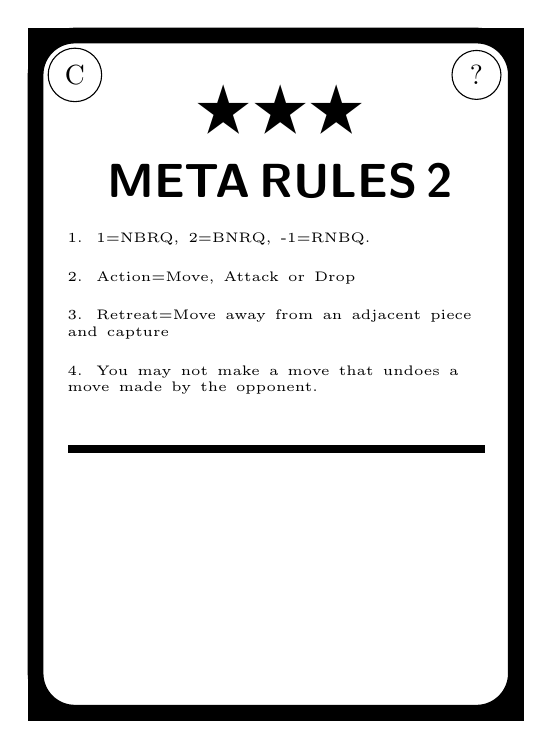
\begin{tikzpicture}
    \pgfmathsetmacro{\cardroundingradius}{5mm}
    \pgfmathsetmacro{\striproundingradius}{3mm}
    % \pgfmathsetmacro{\cardwidth}{5.9}
    % \pgfmathsetmacro{\cardheight}{9.2}
    \pgfmathsetmacro{\cardwidth}{6.1}  % Magic cards are 63x88mm
    \pgfmathsetmacro{\cardheight}{8.6}
    \pgfmathsetmacro{\stripwidth}{1.2}
    \pgfmathsetmacro{\strippadding}{0.1}
    \pgfmathsetmacro{\textpadding}{0.3}
    \pgfmathsetmacro{\ruleheight}{0.1}
    \providecommand{\stripfontsize}{\Huge}
    \providecommand{\captionfontsize}{\LARGE}
    \providecommand{\textfontsize}{\Large}
    \providecommand{\quotefontsize}{\small}
    \draw[line width=2mm,rounded corners=\cardroundingradius] (0,0) rectangle (\cardwidth,\cardheight);
    \draw[line width=2mm] (0,0) rectangle (\cardwidth,\cardheight);
    \node[text width=(\cardwidth-\strippadding-2*\textpadding)*1cm,below right,inner sep=0] at (\strippadding+\textpadding,\cardheight-\textpadding) 
    { 
    \begin{center} {\fontsize{80pt}{60pt}\selectfont \Huge\ding{72}\ding{72}\ding{72}}\\\end{center}
\begin{center}
    {\captionfontsize \textsf{\textbf{META RULES 2}}}\end{center}
        {\textfontsize \tiny
\begin{enumerate}[wide=0pt]
\item 1=NBRQ, 2=BNRQ, -1=RNBQ.\item Action=Move, Attack or Drop\item Retreat=Move away from an adjacent piece and capture\item You may not make a move that undoes a move made by the opponent.\end{enumerate}
}
        \tikz{\fill (0,0) rectangle (\cardwidth-2*\strippadding-2*\textpadding,\ruleheight);}\\
        {\quotefontsize \textit{}}\\[-2\baselineskip]
    };
    \node[circle,draw,text=black](c) at (.5,\cardheight-.5){C};
    \node[circle,draw,text=black](c) at (\cardwidth-.5,\cardheight-.5){?};
    \end{tikzpicture}%
\hspace{1pt}%
\\[-.5\lineskip]
\begin{tikzpicture}
    \pgfmathsetmacro{\cardroundingradius}{5mm}
    \pgfmathsetmacro{\striproundingradius}{3mm}
    % \pgfmathsetmacro{\cardwidth}{5.9}
    % \pgfmathsetmacro{\cardheight}{9.2}
    \pgfmathsetmacro{\cardwidth}{6.1}  % Magic cards are 63x88mm
    \pgfmathsetmacro{\cardheight}{8.6}
    \pgfmathsetmacro{\stripwidth}{1.2}
    \pgfmathsetmacro{\strippadding}{0.1}
    \pgfmathsetmacro{\textpadding}{0.3}
    \pgfmathsetmacro{\ruleheight}{0.1}
    \providecommand{\stripfontsize}{\Huge}
    \providecommand{\captionfontsize}{\LARGE}
    \providecommand{\textfontsize}{\Large}
    \providecommand{\quotefontsize}{\small}
    \draw[line width=2mm,rounded corners=\cardroundingradius] (0,0) rectangle (\cardwidth,\cardheight);
    \draw[line width=2mm] (0,0) rectangle (\cardwidth,\cardheight);
    \node[text width=(\cardwidth-\strippadding-2*\textpadding)*1cm,below right,inner sep=0] at (\strippadding+\textpadding,\cardheight-\textpadding) 
    { 
    \begin{center} {\fontsize{80pt}{60pt}\selectfont \Board+}\\\end{center}
\begin{center}
    {\captionfontsize \textsf{\textbf{10x10 BOARD}}}\end{center}
        {\textfontsize The legal playing area now surrounds the board.}
        \tikz{\fill (0,0) rectangle (\cardwidth-2*\strippadding-2*\textpadding,\ruleheight);}\\
        {\quotefontsize \textit{I don't have anything against walls. You know what it is? I like open spaces. ---Dion Dublin}}\\[-2\baselineskip]
    };
    \node[circle,draw,text=black](c) at (.5,\cardheight-.5){I};
    \node[circle,draw,text=black](c) at (\cardwidth-.5,\cardheight-.5){+};
    \end{tikzpicture}%
\hspace{1pt}%
\begin{tikzpicture}
    \pgfmathsetmacro{\cardroundingradius}{5mm}
    \pgfmathsetmacro{\striproundingradius}{3mm}
    % \pgfmathsetmacro{\cardwidth}{5.9}
    % \pgfmathsetmacro{\cardheight}{9.2}
    \pgfmathsetmacro{\cardwidth}{6.1}  % Magic cards are 63x88mm
    \pgfmathsetmacro{\cardheight}{8.6}
    \pgfmathsetmacro{\stripwidth}{1.2}
    \pgfmathsetmacro{\strippadding}{0.1}
    \pgfmathsetmacro{\textpadding}{0.3}
    \pgfmathsetmacro{\ruleheight}{0.1}
    \providecommand{\stripfontsize}{\Huge}
    \providecommand{\captionfontsize}{\LARGE}
    \providecommand{\textfontsize}{\Large}
    \providecommand{\quotefontsize}{\small}
    \draw[line width=2mm,rounded corners=\cardroundingradius] (0,0) rectangle (\cardwidth,\cardheight);
    \draw[line width=2mm] (0,0) rectangle (\cardwidth,\cardheight);
    \node[text width=(\cardwidth-\strippadding-2*\textpadding)*1cm,below right,inner sep=0] at (\strippadding+\textpadding,\cardheight-\textpadding) 
    { 
    \begin{center} {\fontsize{80pt}{60pt}\selectfont ♗}\\\end{center}
\begin{center}
    {\captionfontsize \textsf{\textbf{BISHOP CHAMPION}}}\end{center}
        {\textfontsize }
        \tikz{\fill (0,0) rectangle (\cardwidth-2*\strippadding-2*\textpadding,\ruleheight);}\\
        {\quotefontsize \textit{\hspace{1cm}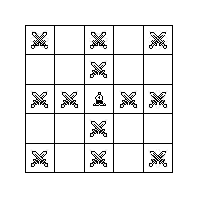
\includegraphics{CHAMPION.pdf}}}\\[-2\baselineskip]
    };
    \node[circle,draw,text=black](c) at (.5,\cardheight-.5){Ω};
    \node[circle,draw,text=black](c) at (\cardwidth-.5,\cardheight-.5){\diff};
    \end{tikzpicture}%
\hspace{1pt}%
\begin{tikzpicture}
    \pgfmathsetmacro{\cardroundingradius}{5mm}
    \pgfmathsetmacro{\striproundingradius}{3mm}
    % \pgfmathsetmacro{\cardwidth}{5.9}
    % \pgfmathsetmacro{\cardheight}{9.2}
    \pgfmathsetmacro{\cardwidth}{6.1}  % Magic cards are 63x88mm
    \pgfmathsetmacro{\cardheight}{8.6}
    \pgfmathsetmacro{\stripwidth}{1.2}
    \pgfmathsetmacro{\strippadding}{0.1}
    \pgfmathsetmacro{\textpadding}{0.3}
    \pgfmathsetmacro{\ruleheight}{0.1}
    \providecommand{\stripfontsize}{\Huge}
    \providecommand{\captionfontsize}{\LARGE}
    \providecommand{\textfontsize}{\Large}
    \providecommand{\quotefontsize}{\small}
    \draw[line width=2mm,rounded corners=\cardroundingradius] (0,0) rectangle (\cardwidth,\cardheight);
    \draw[line width=2mm] (0,0) rectangle (\cardwidth,\cardheight);
    \node[text width=(\cardwidth-\strippadding-2*\textpadding)*1cm,below right,inner sep=0] at (\strippadding+\textpadding,\cardheight-\textpadding) 
    { 
    \begin{center} {\fontsize{80pt}{60pt}\selectfont ♗}\\\end{center}
\begin{center}
    {\captionfontsize \textsf{\textbf{BISHOP COCHAMPION}}}\end{center}
        {\textfontsize }
        \tikz{\fill (0,0) rectangle (\cardwidth-2*\strippadding-2*\textpadding,\ruleheight);}\\
        {\quotefontsize \textit{\hspace{1cm}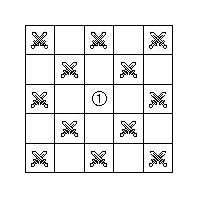
\includegraphics{COCHAMPION.pdf}}}\\[-2\baselineskip]
    };
    \node[circle,draw,text=black](c) at (.5,\cardheight-.5){C};
    \node[circle,draw,text=black](c) at (\cardwidth-.5,\cardheight-.5){\diff};
    \end{tikzpicture}%
\hspace{1pt}%
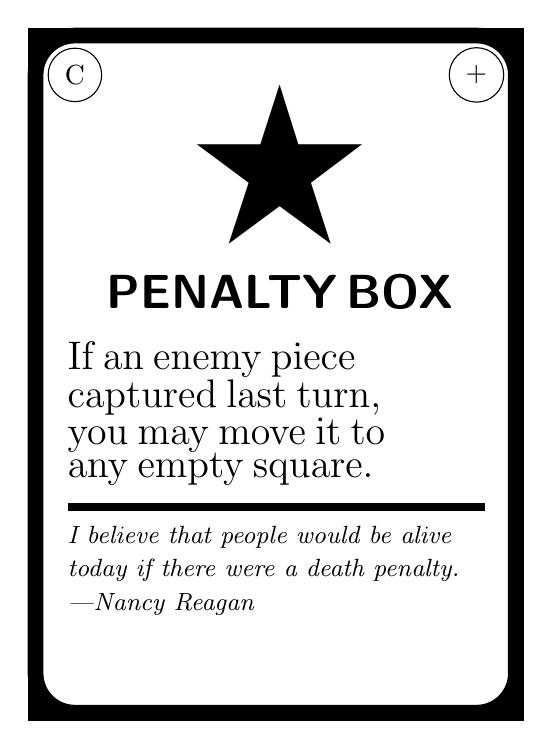
\begin{tikzpicture}
    \pgfmathsetmacro{\cardroundingradius}{5mm}
    \pgfmathsetmacro{\striproundingradius}{3mm}
    % \pgfmathsetmacro{\cardwidth}{5.9}
    % \pgfmathsetmacro{\cardheight}{9.2}
    \pgfmathsetmacro{\cardwidth}{6.1}  % Magic cards are 63x88mm
    \pgfmathsetmacro{\cardheight}{8.6}
    \pgfmathsetmacro{\stripwidth}{1.2}
    \pgfmathsetmacro{\strippadding}{0.1}
    \pgfmathsetmacro{\textpadding}{0.3}
    \pgfmathsetmacro{\ruleheight}{0.1}
    \providecommand{\stripfontsize}{\Huge}
    \providecommand{\captionfontsize}{\LARGE}
    \providecommand{\textfontsize}{\Large}
    \providecommand{\quotefontsize}{\small}
    \draw[line width=2mm,rounded corners=\cardroundingradius] (0,0) rectangle (\cardwidth,\cardheight);
    \draw[line width=2mm] (0,0) rectangle (\cardwidth,\cardheight);
    \node[text width=(\cardwidth-\strippadding-2*\textpadding)*1cm,below right,inner sep=0] at (\strippadding+\textpadding,\cardheight-\textpadding) 
    { 
    \begin{center} {\fontsize{80pt}{60pt}\selectfont \ding{72}}\\\end{center}
\begin{center}
    {\captionfontsize \textsf{\textbf{PENALTY BOX}}}\end{center}
        {\textfontsize If an enemy piece captured last turn, you may move it to any empty square.}
        \tikz{\fill (0,0) rectangle (\cardwidth-2*\strippadding-2*\textpadding,\ruleheight);}\\
        {\quotefontsize \textit{I believe that people would be alive today if there were a death penalty. ---Nancy Reagan}}\\[-2\baselineskip]
    };
    \node[circle,draw,text=black](c) at (.5,\cardheight-.5){C};
    \node[circle,draw,text=black](c) at (\cardwidth-.5,\cardheight-.5){+};
    \end{tikzpicture}%
\hspace{1pt}%
\\[-.5\lineskip]
\begin{tikzpicture}
    \pgfmathsetmacro{\cardroundingradius}{5mm}
    \pgfmathsetmacro{\striproundingradius}{3mm}
    % \pgfmathsetmacro{\cardwidth}{5.9}
    % \pgfmathsetmacro{\cardheight}{9.2}
    \pgfmathsetmacro{\cardwidth}{6.1}  % Magic cards are 63x88mm
    \pgfmathsetmacro{\cardheight}{8.6}
    \pgfmathsetmacro{\stripwidth}{1.2}
    \pgfmathsetmacro{\strippadding}{0.1}
    \pgfmathsetmacro{\textpadding}{0.3}
    \pgfmathsetmacro{\ruleheight}{0.1}
    \providecommand{\stripfontsize}{\Huge}
    \providecommand{\captionfontsize}{\LARGE}
    \providecommand{\textfontsize}{\Large}
    \providecommand{\quotefontsize}{\small}
    \draw[line width=2mm,rounded corners=\cardroundingradius] (0,0) rectangle (\cardwidth,\cardheight);
    \draw[line width=2mm] (0,0) rectangle (\cardwidth,\cardheight);
    \node[text width=(\cardwidth-\strippadding-2*\textpadding)*1cm,below right,inner sep=0] at (\strippadding+\textpadding,\cardheight-\textpadding) 
    { 
    \begin{center} {\fontsize{80pt}{60pt}\selectfont ♘}\\\end{center}
\begin{center}
    {\captionfontsize \textsf{\textbf{MINOR X KNIGHT}}}\end{center}
        {\textfontsize \Sym\Knight$\Move^+\Attack^+$: \PM[1,1]}
        \tikz{\fill (0,0) rectangle (\cardwidth-2*\strippadding-2*\textpadding,\ruleheight);}\\
        {\quotefontsize \textit{\hspace{1cm}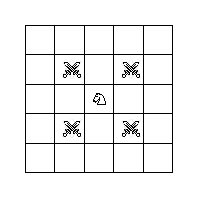
\includegraphics{MINORXKNIGHT.pdf}}}\\[-2\baselineskip]
    };
    \node[circle,draw,text=black](c) at (.5,\cardheight-.5){I};
    \node[circle,draw,text=black](c) at (\cardwidth-.5,\cardheight-.5){+};
    \end{tikzpicture}%
\hspace{1pt}%
\begin{tikzpicture}
    \pgfmathsetmacro{\cardroundingradius}{5mm}
    \pgfmathsetmacro{\striproundingradius}{3mm}
    % \pgfmathsetmacro{\cardwidth}{5.9}
    % \pgfmathsetmacro{\cardheight}{9.2}
    \pgfmathsetmacro{\cardwidth}{6.1}  % Magic cards are 63x88mm
    \pgfmathsetmacro{\cardheight}{8.6}
    \pgfmathsetmacro{\stripwidth}{1.2}
    \pgfmathsetmacro{\strippadding}{0.1}
    \pgfmathsetmacro{\textpadding}{0.3}
    \pgfmathsetmacro{\ruleheight}{0.1}
    \providecommand{\stripfontsize}{\Huge}
    \providecommand{\captionfontsize}{\LARGE}
    \providecommand{\textfontsize}{\Large}
    \providecommand{\quotefontsize}{\small}
    \draw[line width=2mm,rounded corners=\cardroundingradius] (0,0) rectangle (\cardwidth,\cardheight);
    \draw[line width=2mm] (0,0) rectangle (\cardwidth,\cardheight);
    \node[text width=(\cardwidth-\strippadding-2*\textpadding)*1cm,below right,inner sep=0] at (\strippadding+\textpadding,\cardheight-\textpadding) 
    { 
    \begin{center} {\fontsize{80pt}{60pt}\selectfont ♘}\\\end{center}
\begin{center}
    {\captionfontsize \textsf{\textbf{CAVALRY}}}\end{center}
        {\textfontsize A knight can make two captures in one turn.}
        \tikz{\fill (0,0) rectangle (\cardwidth-2*\strippadding-2*\textpadding,\ruleheight);}\\
        {\quotefontsize \textit{It's hard to lead a cavalry charge if you think you look funny on a horse. ---Adlai Stevenson}}\\[-2\baselineskip]
    };
    \node[circle,draw,text=black](c) at (.5,\cardheight-.5){C};
    \node[circle,draw,text=black](c) at (\cardwidth-.5,\cardheight-.5){+};
    \end{tikzpicture}%
\hspace{1pt}%
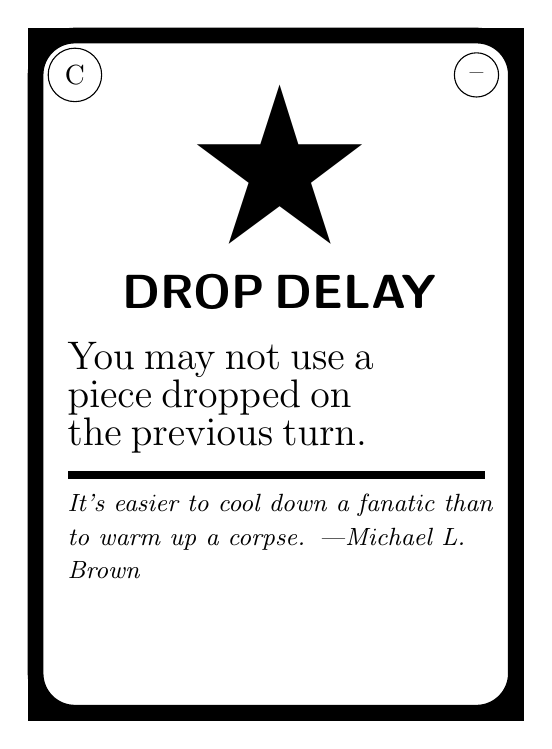
\begin{tikzpicture}
    \pgfmathsetmacro{\cardroundingradius}{5mm}
    \pgfmathsetmacro{\striproundingradius}{3mm}
    % \pgfmathsetmacro{\cardwidth}{5.9}
    % \pgfmathsetmacro{\cardheight}{9.2}
    \pgfmathsetmacro{\cardwidth}{6.1}  % Magic cards are 63x88mm
    \pgfmathsetmacro{\cardheight}{8.6}
    \pgfmathsetmacro{\stripwidth}{1.2}
    \pgfmathsetmacro{\strippadding}{0.1}
    \pgfmathsetmacro{\textpadding}{0.3}
    \pgfmathsetmacro{\ruleheight}{0.1}
    \providecommand{\stripfontsize}{\Huge}
    \providecommand{\captionfontsize}{\LARGE}
    \providecommand{\textfontsize}{\Large}
    \providecommand{\quotefontsize}{\small}
    \draw[line width=2mm,rounded corners=\cardroundingradius] (0,0) rectangle (\cardwidth,\cardheight);
    \draw[line width=2mm] (0,0) rectangle (\cardwidth,\cardheight);
    \node[text width=(\cardwidth-\strippadding-2*\textpadding)*1cm,below right,inner sep=0] at (\strippadding+\textpadding,\cardheight-\textpadding) 
    { 
    \begin{center} {\fontsize{80pt}{60pt}\selectfont \ding{72}}\\\end{center}
\begin{center}
    {\captionfontsize \textsf{\textbf{DROP DELAY}}}\end{center}
        {\textfontsize You may not use a piece dropped on the previous turn.}
        \tikz{\fill (0,0) rectangle (\cardwidth-2*\strippadding-2*\textpadding,\ruleheight);}\\
        {\quotefontsize \textit{It’s easier to cool down a fanatic than to warm up a corpse. ---Michael L. Brown}}\\[-2\baselineskip]
    };
    \node[circle,draw,text=black](c) at (.5,\cardheight-.5){C};
    \node[circle,draw,text=black](c) at (\cardwidth-.5,\cardheight-.5){--};
    \end{tikzpicture}%
\hspace{1pt}%
\begin{tikzpicture}
    \pgfmathsetmacro{\cardroundingradius}{5mm}
    \pgfmathsetmacro{\striproundingradius}{3mm}
    % \pgfmathsetmacro{\cardwidth}{5.9}
    % \pgfmathsetmacro{\cardheight}{9.2}
    \pgfmathsetmacro{\cardwidth}{6.1}  % Magic cards are 63x88mm
    \pgfmathsetmacro{\cardheight}{8.6}
    \pgfmathsetmacro{\stripwidth}{1.2}
    \pgfmathsetmacro{\strippadding}{0.1}
    \pgfmathsetmacro{\textpadding}{0.3}
    \pgfmathsetmacro{\ruleheight}{0.1}
    \providecommand{\stripfontsize}{\Huge}
    \providecommand{\captionfontsize}{\LARGE}
    \providecommand{\textfontsize}{\Large}
    \providecommand{\quotefontsize}{\small}
    \draw[line width=2mm,rounded corners=\cardroundingradius] (0,0) rectangle (\cardwidth,\cardheight);
    \draw[line width=2mm] (0,0) rectangle (\cardwidth,\cardheight);
    \node[text width=(\cardwidth-\strippadding-2*\textpadding)*1cm,below right,inner sep=0] at (\strippadding+\textpadding,\cardheight-\textpadding) 
    { 
    \begin{center} {\fontsize{80pt}{60pt}\selectfont ♘♗}\\\end{center}
\begin{center}
    {\captionfontsize \textsf{\textbf{TRADING PLACES}}}\end{center}
        {\textfontsize You may swap the locations of a friendly knight and bishop for your turn.}
        \tikz{\fill (0,0) rectangle (\cardwidth-2*\strippadding-2*\textpadding,\ruleheight);}\\
        {\quotefontsize \textit{You'll all be very, very sorry. ---Louis Winthorpe}}\\[-2\baselineskip]
    };
    \node[circle,draw,text=black](c) at (.5,\cardheight-.5){C};
    \node[circle,draw,text=black](c) at (\cardwidth-.5,\cardheight-.5){+};
    \end{tikzpicture}%
\hspace{1pt}%
\\[-.5\lineskip]
\begin{tikzpicture}
    \pgfmathsetmacro{\cardroundingradius}{5mm}
    \pgfmathsetmacro{\striproundingradius}{3mm}
    % \pgfmathsetmacro{\cardwidth}{5.9}
    % \pgfmathsetmacro{\cardheight}{9.2}
    \pgfmathsetmacro{\cardwidth}{6.1}  % Magic cards are 63x88mm
    \pgfmathsetmacro{\cardheight}{8.6}
    \pgfmathsetmacro{\stripwidth}{1.2}
    \pgfmathsetmacro{\strippadding}{0.1}
    \pgfmathsetmacro{\textpadding}{0.3}
    \pgfmathsetmacro{\ruleheight}{0.1}
    \providecommand{\stripfontsize}{\Huge}
    \providecommand{\captionfontsize}{\LARGE}
    \providecommand{\textfontsize}{\Large}
    \providecommand{\quotefontsize}{\small}
    \draw[line width=2mm,rounded corners=\cardroundingradius] (0,0) rectangle (\cardwidth,\cardheight);
    \draw[line width=2mm] (0,0) rectangle (\cardwidth,\cardheight);
    \node[text width=(\cardwidth-\strippadding-2*\textpadding)*1cm,below right,inner sep=0] at (\strippadding+\textpadding,\cardheight-\textpadding) 
    { 
    \begin{center} {\fontsize{80pt}{60pt}\selectfont ♙}\\\end{center}
\begin{center}
    {\captionfontsize \textsf{\textbf{CHINESE SHOGI PAWNS}}}\end{center}
        {\textfontsize Pawns take one square forward and move like Chinese checkers. Drop only in file without friendly pawns.}
        \tikz{\fill (0,0) rectangle (\cardwidth-2*\strippadding-2*\textpadding,\ruleheight);}\\
        {\quotefontsize \textit{If there is mate with a Pawn drop, there is a legal mate too. ---Shogi proverb}}\\[-2\baselineskip]
    };
    \node[circle,draw,text=black](c) at (.5,\cardheight-.5){S};
    \node[circle,draw,text=black](c) at (\cardwidth-.5,\cardheight-.5){X};
    \end{tikzpicture}%
\hspace{1pt}%
\begin{tikzpicture}
    \pgfmathsetmacro{\cardroundingradius}{5mm}
    \pgfmathsetmacro{\striproundingradius}{3mm}
    % \pgfmathsetmacro{\cardwidth}{5.9}
    % \pgfmathsetmacro{\cardheight}{9.2}
    \pgfmathsetmacro{\cardwidth}{6.1}  % Magic cards are 63x88mm
    \pgfmathsetmacro{\cardheight}{8.6}
    \pgfmathsetmacro{\stripwidth}{1.2}
    \pgfmathsetmacro{\strippadding}{0.1}
    \pgfmathsetmacro{\textpadding}{0.3}
    \pgfmathsetmacro{\ruleheight}{0.1}
    \providecommand{\stripfontsize}{\Huge}
    \providecommand{\captionfontsize}{\LARGE}
    \providecommand{\textfontsize}{\Large}
    \providecommand{\quotefontsize}{\small}
    \draw[line width=2mm,rounded corners=\cardroundingradius] (0,0) rectangle (\cardwidth,\cardheight);
    \draw[line width=2mm] (0,0) rectangle (\cardwidth,\cardheight);
    \node[text width=(\cardwidth-\strippadding-2*\textpadding)*1cm,below right,inner sep=0] at (\strippadding+\textpadding,\cardheight-\textpadding) 
    { 
    \begin{center} {\fontsize{80pt}{60pt}\selectfont ♗}\\\end{center}
\begin{center}
    {\captionfontsize \textsf{\textbf{RETREATER}}}\end{center}
        {\textfontsize \Sym\Bishop$\Move$: \Queen\Move\newline\Sym\Bishop$\Attack$: \Back\Queen\Move}
        \tikz{\fill (0,0) rectangle (\cardwidth-2*\strippadding-2*\textpadding,\ruleheight);}\\
        {\quotefontsize \textit{He who fights and runs away, lives to fight another day. ---Proverb}}\\[-2\baselineskip]
    };
    \node[circle,draw,text=black](c) at (.5,\cardheight-.5){U};
    \node[circle,draw,text=black](c) at (\cardwidth-.5,\cardheight-.5){X};
    \end{tikzpicture}%
\hspace{1pt}%
\begin{tikzpicture}
    \pgfmathsetmacro{\cardroundingradius}{5mm}
    \pgfmathsetmacro{\striproundingradius}{3mm}
    % \pgfmathsetmacro{\cardwidth}{5.9}
    % \pgfmathsetmacro{\cardheight}{9.2}
    \pgfmathsetmacro{\cardwidth}{6.1}  % Magic cards are 63x88mm
    \pgfmathsetmacro{\cardheight}{8.6}
    \pgfmathsetmacro{\stripwidth}{1.2}
    \pgfmathsetmacro{\strippadding}{0.1}
    \pgfmathsetmacro{\textpadding}{0.3}
    \pgfmathsetmacro{\ruleheight}{0.1}
    \providecommand{\stripfontsize}{\Huge}
    \providecommand{\captionfontsize}{\LARGE}
    \providecommand{\textfontsize}{\Large}
    \providecommand{\quotefontsize}{\small}
    \draw[line width=2mm,rounded corners=\cardroundingradius] (0,0) rectangle (\cardwidth,\cardheight);
    \draw[line width=2mm] (0,0) rectangle (\cardwidth,\cardheight);
    \node[text width=(\cardwidth-\strippadding-2*\textpadding)*1cm,below right,inner sep=0] at (\strippadding+\textpadding,\cardheight-\textpadding) 
    { 
    \begin{center} {\fontsize{80pt}{60pt}\selectfont ♗}\\\end{center}
\begin{center}
    {\captionfontsize \textsf{\textbf{BISHOP LONG LEAPER}}}\end{center}
        {\textfontsize \Sym\Bishop$\Move$: \Queen\Move\newline\Sym\Bishop$\Attack$: \Jump\Queen\Move}
        \tikz{\fill (0,0) rectangle (\cardwidth-2*\strippadding-2*\textpadding,\ruleheight);}\\
        {\quotefontsize \textit{That's one small step for a man, one giant leap for mankind. ---Neil Armstrong}}\\[-2\baselineskip]
    };
    \node[circle,draw,text=black](c) at (.5,\cardheight-.5){U};
    \node[circle,draw,text=black](c) at (\cardwidth-.5,\cardheight-.5){?};
    \end{tikzpicture}%
\hspace{1pt}%
\begin{tikzpicture}
    \pgfmathsetmacro{\cardroundingradius}{5mm}
    \pgfmathsetmacro{\striproundingradius}{3mm}
    % \pgfmathsetmacro{\cardwidth}{5.9}
    % \pgfmathsetmacro{\cardheight}{9.2}
    \pgfmathsetmacro{\cardwidth}{6.1}  % Magic cards are 63x88mm
    \pgfmathsetmacro{\cardheight}{8.6}
    \pgfmathsetmacro{\stripwidth}{1.2}
    \pgfmathsetmacro{\strippadding}{0.1}
    \pgfmathsetmacro{\textpadding}{0.3}
    \pgfmathsetmacro{\ruleheight}{0.1}
    \providecommand{\stripfontsize}{\Huge}
    \providecommand{\captionfontsize}{\LARGE}
    \providecommand{\textfontsize}{\Large}
    \providecommand{\quotefontsize}{\small}
    \draw[line width=2mm,rounded corners=\cardroundingradius] (0,0) rectangle (\cardwidth,\cardheight);
    \draw[line width=2mm] (0,0) rectangle (\cardwidth,\cardheight);
    \node[text width=(\cardwidth-\strippadding-2*\textpadding)*1cm,below right,inner sep=0] at (\strippadding+\textpadding,\cardheight-\textpadding) 
    { 
    \begin{center} {\fontsize{80pt}{60pt}\selectfont ♙♔}\\\end{center}
\begin{center}
    {\captionfontsize \textsf{\textbf{IT FOLLOWS}}}\end{center}
        {\textfontsize After moving a non-pawn piece, the closest $L_1$ norm pawn to the opponent's king moves one space forward.}
        \tikz{\fill (0,0) rectangle (\cardwidth-2*\strippadding-2*\textpadding,\ruleheight);}\\
        {\quotefontsize \textit{Love make us poets, and the approach of death should make us philosophers.---George Santayana}}\\[-2\baselineskip]
    };
    \node[circle,draw,text=black](c) at (.5,\cardheight-.5){C};
    \node[circle,draw,text=black](c) at (\cardwidth-.5,\cardheight-.5){?};
    \end{tikzpicture}%
\hspace{1pt}%
\\[-.5\lineskip]
\begin{tikzpicture}
    \pgfmathsetmacro{\cardroundingradius}{5mm}
    \pgfmathsetmacro{\striproundingradius}{3mm}
    % \pgfmathsetmacro{\cardwidth}{5.9}
    % \pgfmathsetmacro{\cardheight}{9.2}
    \pgfmathsetmacro{\cardwidth}{6.1}  % Magic cards are 63x88mm
    \pgfmathsetmacro{\cardheight}{8.6}
    \pgfmathsetmacro{\stripwidth}{1.2}
    \pgfmathsetmacro{\strippadding}{0.1}
    \pgfmathsetmacro{\textpadding}{0.3}
    \pgfmathsetmacro{\ruleheight}{0.1}
    \providecommand{\stripfontsize}{\Huge}
    \providecommand{\captionfontsize}{\LARGE}
    \providecommand{\textfontsize}{\Large}
    \providecommand{\quotefontsize}{\small}
    \draw[line width=2mm,rounded corners=\cardroundingradius] (0,0) rectangle (\cardwidth,\cardheight);
    \draw[line width=2mm] (0,0) rectangle (\cardwidth,\cardheight);
    \node[text width=(\cardwidth-\strippadding-2*\textpadding)*1cm,below right,inner sep=0] at (\strippadding+\textpadding,\cardheight-\textpadding) 
    { 
    \begin{center} {\fontsize{80pt}{60pt}\selectfont ♗}\\\end{center}
\begin{center}
    {\captionfontsize \textsf{\textbf{CROWNED LONG LEAPER}}}\end{center}
        {\textfontsize \Sym\Bishop$\Move$: \Queen\Move\newline\Sym\Bishop$\Attack$: \Jump\Queen\Move\newline\Sym\Bishop$\Attack$: \King\Attack}
        \tikz{\fill (0,0) rectangle (\cardwidth-2*\strippadding-2*\textpadding,\ruleheight);}\\
        {\quotefontsize \textit{Jump! ---Van Halen}}\\[-2\baselineskip]
    };
    \node[circle,draw,text=black](c) at (.5,\cardheight-.5){C};
    \node[circle,draw,text=black](c) at (\cardwidth-.5,\cardheight-.5){?};
    \end{tikzpicture}%
\hspace{1pt}%
\begin{tikzpicture}
    \pgfmathsetmacro{\cardroundingradius}{5mm}
    \pgfmathsetmacro{\striproundingradius}{3mm}
    % \pgfmathsetmacro{\cardwidth}{5.9}
    % \pgfmathsetmacro{\cardheight}{9.2}
    \pgfmathsetmacro{\cardwidth}{6.1}  % Magic cards are 63x88mm
    \pgfmathsetmacro{\cardheight}{8.6}
    \pgfmathsetmacro{\stripwidth}{1.2}
    \pgfmathsetmacro{\strippadding}{0.1}
    \pgfmathsetmacro{\textpadding}{0.3}
    \pgfmathsetmacro{\ruleheight}{0.1}
    \providecommand{\stripfontsize}{\Huge}
    \providecommand{\captionfontsize}{\LARGE}
    \providecommand{\textfontsize}{\Large}
    \providecommand{\quotefontsize}{\small}
    \draw[line width=2mm,rounded corners=\cardroundingradius] (0,0) rectangle (\cardwidth,\cardheight);
    \draw[line width=2mm] (0,0) rectangle (\cardwidth,\cardheight);
    \node[text width=(\cardwidth-\strippadding-2*\textpadding)*1cm,below right,inner sep=0] at (\strippadding+\textpadding,\cardheight-\textpadding) 
    { 
    \begin{center} {\fontsize{80pt}{60pt}\selectfont ♗}\\\end{center}
\begin{center}
    {\captionfontsize \textsf{\textbf{CROWNED RETREATER}}}\end{center}
        {\textfontsize \Sym\Bishop$\Move$: \Queen\Move\newline\Sym\Bishop$\Attack$: \Back\Queen\Move\newline\Sym\Bishop$\Attack$: \King\Attack}
        \tikz{\fill (0,0) rectangle (\cardwidth-2*\strippadding-2*\textpadding,\ruleheight);}\\
        {\quotefontsize \textit{He who fights and runs away, lives to fight another day. ---Proverb}}\\[-2\baselineskip]
    };
    \node[circle,draw,text=black](c) at (.5,\cardheight-.5){C};
    \node[circle,draw,text=black](c) at (\cardwidth-.5,\cardheight-.5){?};
    \end{tikzpicture}%
\hspace{1pt}%
\begin{tikzpicture}
    \pgfmathsetmacro{\cardroundingradius}{5mm}
    \pgfmathsetmacro{\striproundingradius}{3mm}
    % \pgfmathsetmacro{\cardwidth}{5.9}
    % \pgfmathsetmacro{\cardheight}{9.2}
    \pgfmathsetmacro{\cardwidth}{6.1}  % Magic cards are 63x88mm
    \pgfmathsetmacro{\cardheight}{8.6}
    \pgfmathsetmacro{\stripwidth}{1.2}
    \pgfmathsetmacro{\strippadding}{0.1}
    \pgfmathsetmacro{\textpadding}{0.3}
    \pgfmathsetmacro{\ruleheight}{0.1}
    \providecommand{\stripfontsize}{\Huge}
    \providecommand{\captionfontsize}{\LARGE}
    \providecommand{\textfontsize}{\Large}
    \providecommand{\quotefontsize}{\small}
    \draw[line width=2mm,rounded corners=\cardroundingradius] (0,0) rectangle (\cardwidth,\cardheight);
    \draw[line width=2mm] (0,0) rectangle (\cardwidth,\cardheight);
    \node[text width=(\cardwidth-\strippadding-2*\textpadding)*1cm,below right,inner sep=0] at (\strippadding+\textpadding,\cardheight-\textpadding) 
    { 
    \begin{center} {\fontsize{80pt}{60pt}\selectfont ♙+}\\\end{center}
\begin{center}
    {\captionfontsize \textsf{\textbf{SHOGI PAWNS}}}\end{center}
        {\textfontsize Pawns take one square forward and may not move two squares initially. Drop only in file without friendly pawns.}
        \tikz{\fill (0,0) rectangle (\cardwidth-2*\strippadding-2*\textpadding,\ruleheight);}\\
        {\quotefontsize \textit{If there is mate with a Pawn drop, there is a legal mate too. ---Shogi proverb}}\\[-2\baselineskip]
    };
    \node[circle,draw,text=black](c) at (.5,\cardheight-.5){S};
    \node[circle,draw,text=black](c) at (\cardwidth-.5,\cardheight-.5){?};
    \end{tikzpicture}%
\hspace{1pt}%
\begin{tikzpicture}
    \pgfmathsetmacro{\cardroundingradius}{5mm}
    \pgfmathsetmacro{\striproundingradius}{3mm}
    % \pgfmathsetmacro{\cardwidth}{5.9}
    % \pgfmathsetmacro{\cardheight}{9.2}
    \pgfmathsetmacro{\cardwidth}{6.1}  % Magic cards are 63x88mm
    \pgfmathsetmacro{\cardheight}{8.6}
    \pgfmathsetmacro{\stripwidth}{1.2}
    \pgfmathsetmacro{\strippadding}{0.1}
    \pgfmathsetmacro{\textpadding}{0.3}
    \pgfmathsetmacro{\ruleheight}{0.1}
    \providecommand{\stripfontsize}{\Huge}
    \providecommand{\captionfontsize}{\LARGE}
    \providecommand{\textfontsize}{\Large}
    \providecommand{\quotefontsize}{\small}
    \draw[line width=2mm,rounded corners=\cardroundingradius] (0,0) rectangle (\cardwidth,\cardheight);
    \draw[line width=2mm] (0,0) rectangle (\cardwidth,\cardheight);
    \node[text width=(\cardwidth-\strippadding-2*\textpadding)*1cm,below right,inner sep=0] at (\strippadding+\textpadding,\cardheight-\textpadding) 
    { 
    \begin{center} {\fontsize{80pt}{60pt}\selectfont ♕}\\\end{center}
\begin{center}
    {\captionfontsize \textsf{\textbf{NIGHT KING QUEEN}}}\end{center}
        {\textfontsize \Sym\Queen\Move: (\Knight+\King)\Move\newline\Sym\Queen\Attack: (\Knight+\King)\Attack}
        \tikz{\fill (0,0) rectangle (\cardwidth-2*\strippadding-2*\textpadding,\ruleheight);}\\
        {\quotefontsize \textit{Night's King was only a man by light of day, Old Nan would always say, but the night was his to rule. ---Brandon Stark}}\\[-2\baselineskip]
    };
    \node[circle,draw,text=black](c) at (.5,\cardheight-.5){?};
    \node[circle,draw,text=black](c) at (\cardwidth-.5,\cardheight-.5){?};
    \end{tikzpicture}%
\hspace{1pt}%
\\[-.5\lineskip]
\begin{tikzpicture}
    \pgfmathsetmacro{\cardroundingradius}{5mm}
    \pgfmathsetmacro{\striproundingradius}{3mm}
    % \pgfmathsetmacro{\cardwidth}{5.9}
    % \pgfmathsetmacro{\cardheight}{9.2}
    \pgfmathsetmacro{\cardwidth}{6.1}  % Magic cards are 63x88mm
    \pgfmathsetmacro{\cardheight}{8.6}
    \pgfmathsetmacro{\stripwidth}{1.2}
    \pgfmathsetmacro{\strippadding}{0.1}
    \pgfmathsetmacro{\textpadding}{0.3}
    \pgfmathsetmacro{\ruleheight}{0.1}
    \providecommand{\stripfontsize}{\Huge}
    \providecommand{\captionfontsize}{\LARGE}
    \providecommand{\textfontsize}{\Large}
    \providecommand{\quotefontsize}{\small}
    \draw[line width=2mm,rounded corners=\cardroundingradius] (0,0) rectangle (\cardwidth,\cardheight);
    \draw[line width=2mm] (0,0) rectangle (\cardwidth,\cardheight);
    \node[text width=(\cardwidth-\strippadding-2*\textpadding)*1cm,below right,inner sep=0] at (\strippadding+\textpadding,\cardheight-\textpadding) 
    { 
    \begin{center} {\fontsize{80pt}{60pt}\selectfont ♖}\\\end{center}
\begin{center}
    {\captionfontsize \textsf{\textbf{CROWNED CASTLE}}}\end{center}
        {\textfontsize \Sym\Rook$\Move^+$: \King\Move\newline\Sym\Rook$\Attack^+$: \King\Attack}
        \tikz{\fill (0,0) rectangle (\cardwidth-2*\strippadding-2*\textpadding,\ruleheight);}\\
        {\quotefontsize \textit{In the land of the skunks, he who has half a nose is king. ---Chris Farley}}\\[-2\baselineskip]
    };
    \node[circle,draw,text=black](c) at (.5,\cardheight-.5){I};
    \node[circle,draw,text=black](c) at (\cardwidth-.5,\cardheight-.5){?};
    \end{tikzpicture}%
\hspace{1pt}%
\begin{tikzpicture}
    \pgfmathsetmacro{\cardroundingradius}{5mm}
    \pgfmathsetmacro{\striproundingradius}{3mm}
    % \pgfmathsetmacro{\cardwidth}{5.9}
    % \pgfmathsetmacro{\cardheight}{9.2}
    \pgfmathsetmacro{\cardwidth}{6.1}  % Magic cards are 63x88mm
    \pgfmathsetmacro{\cardheight}{8.6}
    \pgfmathsetmacro{\stripwidth}{1.2}
    \pgfmathsetmacro{\strippadding}{0.1}
    \pgfmathsetmacro{\textpadding}{0.3}
    \pgfmathsetmacro{\ruleheight}{0.1}
    \providecommand{\stripfontsize}{\Huge}
    \providecommand{\captionfontsize}{\LARGE}
    \providecommand{\textfontsize}{\Large}
    \providecommand{\quotefontsize}{\small}
    \draw[line width=2mm,rounded corners=\cardroundingradius] (0,0) rectangle (\cardwidth,\cardheight);
    \draw[line width=2mm] (0,0) rectangle (\cardwidth,\cardheight);
    \node[text width=(\cardwidth-\strippadding-2*\textpadding)*1cm,below right,inner sep=0] at (\strippadding+\textpadding,\cardheight-\textpadding) 
    { 
    \begin{center} {\fontsize{80pt}{60pt}\selectfont ♗}\\\end{center}
\begin{center}
    {\captionfontsize \textsf{\textbf{CROWNED BISHOP}}}\end{center}
        {\textfontsize \Sym\Bishop$\Move^+$: \King\Move\newline\Sym\Bishop$\Attack^+$: \King\Attack}
        \tikz{\fill (0,0) rectangle (\cardwidth-2*\strippadding-2*\textpadding,\ruleheight);}\\
        {\quotefontsize \textit{In the land of the blind the one-eyed man is king. ---Efren Ramirez}}\\[-2\baselineskip]
    };
    \node[circle,draw,text=black](c) at (.5,\cardheight-.5){I};
    \node[circle,draw,text=black](c) at (\cardwidth-.5,\cardheight-.5){?};
    \end{tikzpicture}%
\hspace{1pt}%
\begin{tikzpicture}
    \pgfmathsetmacro{\cardroundingradius}{5mm}
    \pgfmathsetmacro{\striproundingradius}{3mm}
    % \pgfmathsetmacro{\cardwidth}{5.9}
    % \pgfmathsetmacro{\cardheight}{9.2}
    \pgfmathsetmacro{\cardwidth}{6.1}  % Magic cards are 63x88mm
    \pgfmathsetmacro{\cardheight}{8.6}
    \pgfmathsetmacro{\stripwidth}{1.2}
    \pgfmathsetmacro{\strippadding}{0.1}
    \pgfmathsetmacro{\textpadding}{0.3}
    \pgfmathsetmacro{\ruleheight}{0.1}
    \providecommand{\stripfontsize}{\Huge}
    \providecommand{\captionfontsize}{\LARGE}
    \providecommand{\textfontsize}{\Large}
    \providecommand{\quotefontsize}{\small}
    \draw[line width=2mm,rounded corners=\cardroundingradius] (0,0) rectangle (\cardwidth,\cardheight);
    \draw[line width=2mm] (0,0) rectangle (\cardwidth,\cardheight);
    \node[text width=(\cardwidth-\strippadding-2*\textpadding)*1cm,below right,inner sep=0] at (\strippadding+\textpadding,\cardheight-\textpadding) 
    { 
    \begin{center} {\fontsize{80pt}{60pt}\selectfont ♘}\\\end{center}
\begin{center}
    {\captionfontsize \textsf{\textbf{NIGHT WIZARD}}}\end{center}
        {\textfontsize \Sym\Knight\Move: ±[1,1],[1,3]\newline \Knight\Attack: \Same}
        \tikz{\fill (0,0) rectangle (\cardwidth-2*\strippadding-2*\textpadding,\ruleheight);}\\
        {\quotefontsize \textit{Do not meddle in the affairs of Wizards, for they are subtle and quick to anger. ---J. R. R. Tolkien}}\\[-2\baselineskip]
    };
    \node[circle,draw,text=black](c) at (.5,\cardheight-.5){Ω};
    \node[circle,draw,text=black](c) at (\cardwidth-.5,\cardheight-.5){?};
    \end{tikzpicture}%
\hspace{1pt}%
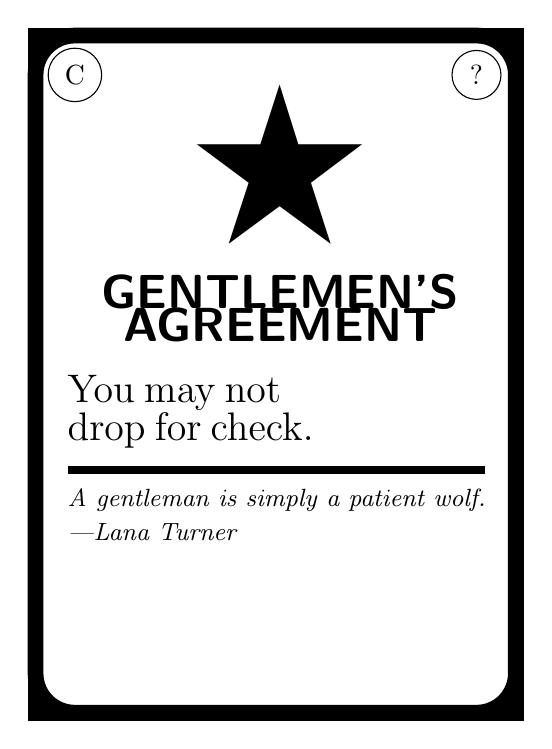
\begin{tikzpicture}
    \pgfmathsetmacro{\cardroundingradius}{5mm}
    \pgfmathsetmacro{\striproundingradius}{3mm}
    % \pgfmathsetmacro{\cardwidth}{5.9}
    % \pgfmathsetmacro{\cardheight}{9.2}
    \pgfmathsetmacro{\cardwidth}{6.1}  % Magic cards are 63x88mm
    \pgfmathsetmacro{\cardheight}{8.6}
    \pgfmathsetmacro{\stripwidth}{1.2}
    \pgfmathsetmacro{\strippadding}{0.1}
    \pgfmathsetmacro{\textpadding}{0.3}
    \pgfmathsetmacro{\ruleheight}{0.1}
    \providecommand{\stripfontsize}{\Huge}
    \providecommand{\captionfontsize}{\LARGE}
    \providecommand{\textfontsize}{\Large}
    \providecommand{\quotefontsize}{\small}
    \draw[line width=2mm,rounded corners=\cardroundingradius] (0,0) rectangle (\cardwidth,\cardheight);
    \draw[line width=2mm] (0,0) rectangle (\cardwidth,\cardheight);
    \node[text width=(\cardwidth-\strippadding-2*\textpadding)*1cm,below right,inner sep=0] at (\strippadding+\textpadding,\cardheight-\textpadding) 
    { 
    \begin{center} {\fontsize{80pt}{60pt}\selectfont \ding{72}}\\\end{center}
\begin{center}
    {\captionfontsize \textsf{\textbf{GENTLEMEN'S AGREEMENT}}}\end{center}
        {\textfontsize You may not drop for check.}
        \tikz{\fill (0,0) rectangle (\cardwidth-2*\strippadding-2*\textpadding,\ruleheight);}\\
        {\quotefontsize \textit{A gentleman is simply a patient wolf. ---Lana Turner}}\\[-2\baselineskip]
    };
    \node[circle,draw,text=black](c) at (.5,\cardheight-.5){C};
    \node[circle,draw,text=black](c) at (\cardwidth-.5,\cardheight-.5){?};
    \end{tikzpicture}%
\hspace{1pt}%
\\[-.5\lineskip]
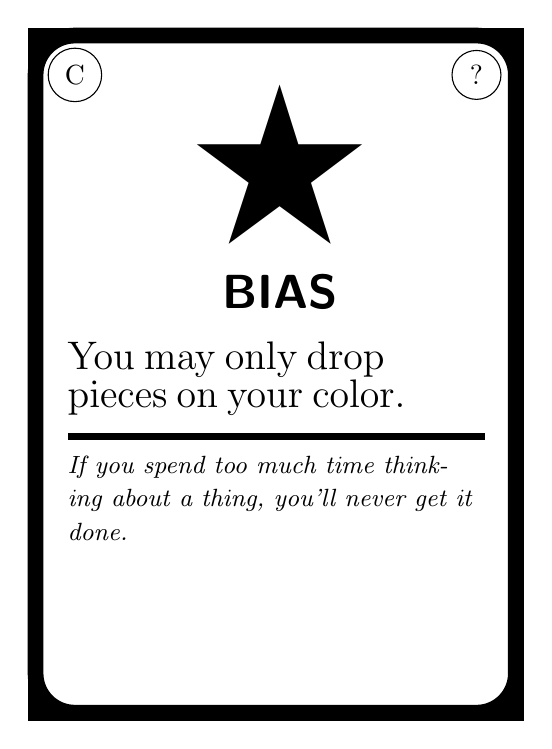
\begin{tikzpicture}
    \pgfmathsetmacro{\cardroundingradius}{5mm}
    \pgfmathsetmacro{\striproundingradius}{3mm}
    % \pgfmathsetmacro{\cardwidth}{5.9}
    % \pgfmathsetmacro{\cardheight}{9.2}
    \pgfmathsetmacro{\cardwidth}{6.1}  % Magic cards are 63x88mm
    \pgfmathsetmacro{\cardheight}{8.6}
    \pgfmathsetmacro{\stripwidth}{1.2}
    \pgfmathsetmacro{\strippadding}{0.1}
    \pgfmathsetmacro{\textpadding}{0.3}
    \pgfmathsetmacro{\ruleheight}{0.1}
    \providecommand{\stripfontsize}{\Huge}
    \providecommand{\captionfontsize}{\LARGE}
    \providecommand{\textfontsize}{\Large}
    \providecommand{\quotefontsize}{\small}
    \draw[line width=2mm,rounded corners=\cardroundingradius] (0,0) rectangle (\cardwidth,\cardheight);
    \draw[line width=2mm] (0,0) rectangle (\cardwidth,\cardheight);
    \node[text width=(\cardwidth-\strippadding-2*\textpadding)*1cm,below right,inner sep=0] at (\strippadding+\textpadding,\cardheight-\textpadding) 
    { 
    \begin{center} {\fontsize{80pt}{60pt}\selectfont \ding{72}}\\\end{center}
\begin{center}
    {\captionfontsize \textsf{\textbf{BIAS}}}\end{center}
        {\textfontsize You may only drop pieces on your color.}
        \tikz{\fill (0,0) rectangle (\cardwidth-2*\strippadding-2*\textpadding,\ruleheight);}\\
        {\quotefontsize \textit{If you spend too much time thinking about a thing, you'll never get it done.}}\\[-2\baselineskip]
    };
    \node[circle,draw,text=black](c) at (.5,\cardheight-.5){C};
    \node[circle,draw,text=black](c) at (\cardwidth-.5,\cardheight-.5){?};
    \end{tikzpicture}%
\hspace{1pt}%
\begin{tikzpicture}
    \pgfmathsetmacro{\cardroundingradius}{5mm}
    \pgfmathsetmacro{\striproundingradius}{3mm}
    % \pgfmathsetmacro{\cardwidth}{5.9}
    % \pgfmathsetmacro{\cardheight}{9.2}
    \pgfmathsetmacro{\cardwidth}{6.1}  % Magic cards are 63x88mm
    \pgfmathsetmacro{\cardheight}{8.6}
    \pgfmathsetmacro{\stripwidth}{1.2}
    \pgfmathsetmacro{\strippadding}{0.1}
    \pgfmathsetmacro{\textpadding}{0.3}
    \pgfmathsetmacro{\ruleheight}{0.1}
    \providecommand{\stripfontsize}{\Huge}
    \providecommand{\captionfontsize}{\LARGE}
    \providecommand{\textfontsize}{\Large}
    \providecommand{\quotefontsize}{\small}
    \draw[line width=2mm,rounded corners=\cardroundingradius] (0,0) rectangle (\cardwidth,\cardheight);
    \draw[line width=2mm] (0,0) rectangle (\cardwidth,\cardheight);
    \node[text width=(\cardwidth-\strippadding-2*\textpadding)*1cm,below right,inner sep=0] at (\strippadding+\textpadding,\cardheight-\textpadding) 
    { 
    \begin{center} {\fontsize{80pt}{60pt}\selectfont ♘♗}\\\end{center}
\begin{center}
    {\captionfontsize \textsf{\textbf{BISHOP-KNIGHT SWAP}}}\end{center}
        {\textfontsize \Sym\Knight\Attack: \Bishop\Attack\newline\Bishop\Attack: \Knight\Attack}
        \tikz{\fill (0,0) rectangle (\cardwidth-2*\strippadding-2*\textpadding,\ruleheight);}\\
        {\quotefontsize \textit{It's time to bait a trap. ---Katie Reus}}\\[-2\baselineskip]
    };
    \node[circle,draw,text=black](c) at (.5,\cardheight-.5){?};
    \node[circle,draw,text=black](c) at (\cardwidth-.5,\cardheight-.5){?};
    \end{tikzpicture}%
\hspace{1pt}%
\begin{tikzpicture}
    \pgfmathsetmacro{\cardroundingradius}{5mm}
    \pgfmathsetmacro{\striproundingradius}{3mm}
    % \pgfmathsetmacro{\cardwidth}{5.9}
    % \pgfmathsetmacro{\cardheight}{9.2}
    \pgfmathsetmacro{\cardwidth}{6.1}  % Magic cards are 63x88mm
    \pgfmathsetmacro{\cardheight}{8.6}
    \pgfmathsetmacro{\stripwidth}{1.2}
    \pgfmathsetmacro{\strippadding}{0.1}
    \pgfmathsetmacro{\textpadding}{0.3}
    \pgfmathsetmacro{\ruleheight}{0.1}
    \providecommand{\stripfontsize}{\Huge}
    \providecommand{\captionfontsize}{\LARGE}
    \providecommand{\textfontsize}{\Large}
    \providecommand{\quotefontsize}{\small}
    \draw[line width=2mm,rounded corners=\cardroundingradius] (0,0) rectangle (\cardwidth,\cardheight);
    \draw[line width=2mm] (0,0) rectangle (\cardwidth,\cardheight);
    \node[text width=(\cardwidth-\strippadding-2*\textpadding)*1cm,below right,inner sep=0] at (\strippadding+\textpadding,\cardheight-\textpadding) 
    { 
    \begin{center} {\fontsize{80pt}{60pt}\selectfont ♘♗}\\\end{center}
\begin{center}
    {\captionfontsize \textsf{\textbf{PRISON BREAK}}}\end{center}
        {\textfontsize \small All knights start off the board in jail. If a bishop moves/attacks, ending on the last rank, knights of the same color are now available to be dropped by the owner.}
        \tikz{\fill (0,0) rectangle (\cardwidth-2*\strippadding-2*\textpadding,\ruleheight);}\\
        {\quotefontsize \textit{\tiny Preparation can only take you so far. After that, you have to take a few leaps of faith. ---Michael Scofield}}\\[-2\baselineskip]
    };
    \node[circle,draw,text=black](c) at (.5,\cardheight-.5){C};
    \node[circle,draw,text=black](c) at (\cardwidth-.5,\cardheight-.5){?};
    \end{tikzpicture}%
\hspace{1pt}%
\begin{tikzpicture}
    \pgfmathsetmacro{\cardroundingradius}{5mm}
    \pgfmathsetmacro{\striproundingradius}{3mm}
    % \pgfmathsetmacro{\cardwidth}{5.9}
    % \pgfmathsetmacro{\cardheight}{9.2}
    \pgfmathsetmacro{\cardwidth}{6.1}  % Magic cards are 63x88mm
    \pgfmathsetmacro{\cardheight}{8.6}
    \pgfmathsetmacro{\stripwidth}{1.2}
    \pgfmathsetmacro{\strippadding}{0.1}
    \pgfmathsetmacro{\textpadding}{0.3}
    \pgfmathsetmacro{\ruleheight}{0.1}
    \providecommand{\stripfontsize}{\Huge}
    \providecommand{\captionfontsize}{\LARGE}
    \providecommand{\textfontsize}{\Large}
    \providecommand{\quotefontsize}{\small}
    \draw[line width=2mm,rounded corners=\cardroundingradius] (0,0) rectangle (\cardwidth,\cardheight);
    \draw[line width=2mm] (0,0) rectangle (\cardwidth,\cardheight);
    \node[text width=(\cardwidth-\strippadding-2*\textpadding)*1cm,below right,inner sep=0] at (\strippadding+\textpadding,\cardheight-\textpadding) 
    { 
    \begin{center} {\fontsize{80pt}{60pt}\selectfont ♕}\\\end{center}
\begin{center}
    {\captionfontsize \textsf{\textbf{REARGUARD}}}\end{center}
        {\textfontsize Whenever a Queen moves (not drop), it may summon a pawn to the square behind it.}
        \tikz{\fill (0,0) rectangle (\cardwidth-2*\strippadding-2*\textpadding,\ruleheight);}\\
        {\quotefontsize \textit{If you think you're going to be a backup, you're going to be a backup. ---Nick Foles}}\\[-2\baselineskip]
    };
    \node[circle,draw,text=black](c) at (.5,\cardheight-.5){?};
    \node[circle,draw,text=black](c) at (\cardwidth-.5,\cardheight-.5){?};
    \end{tikzpicture}%
\hspace{1pt}%
\\[-.5\lineskip]
\begin{tikzpicture}
    \pgfmathsetmacro{\cardroundingradius}{5mm}
    \pgfmathsetmacro{\striproundingradius}{3mm}
    % \pgfmathsetmacro{\cardwidth}{5.9}
    % \pgfmathsetmacro{\cardheight}{9.2}
    \pgfmathsetmacro{\cardwidth}{6.1}  % Magic cards are 63x88mm
    \pgfmathsetmacro{\cardheight}{8.6}
    \pgfmathsetmacro{\stripwidth}{1.2}
    \pgfmathsetmacro{\strippadding}{0.1}
    \pgfmathsetmacro{\textpadding}{0.3}
    \pgfmathsetmacro{\ruleheight}{0.1}
    \providecommand{\stripfontsize}{\Huge}
    \providecommand{\captionfontsize}{\LARGE}
    \providecommand{\textfontsize}{\Large}
    \providecommand{\quotefontsize}{\small}
    \draw[line width=2mm,rounded corners=\cardroundingradius] (0,0) rectangle (\cardwidth,\cardheight);
    \draw[line width=2mm] (0,0) rectangle (\cardwidth,\cardheight);
    \node[text width=(\cardwidth-\strippadding-2*\textpadding)*1cm,below right,inner sep=0] at (\strippadding+\textpadding,\cardheight-\textpadding) 
    { 
    \begin{center} {\fontsize{80pt}{60pt}\selectfont \ding{72}}\\\end{center}
\begin{center}
    {\captionfontsize \textsf{\textbf{UNFAIR}}}\end{center}
        {\textfontsize Deal a card. It only applies to white. Deal a second card. It only applies to black. Deal with it.}
        \tikz{\fill (0,0) rectangle (\cardwidth-2*\strippadding-2*\textpadding,\ruleheight);}\\
        {\quotefontsize \textit{I know the world isn't fair, but why isn't it ever unfair in my favor? ---Bill Watterson}}\\[-2\baselineskip]
    };
    \node[circle,draw,text=black](c) at (.5,\cardheight-.5){C};
    \node[circle,draw,text=black](c) at (\cardwidth-.5,\cardheight-.5){?};
    \end{tikzpicture}%
\hspace{1pt}%
\begin{tikzpicture}
    \pgfmathsetmacro{\cardroundingradius}{5mm}
    \pgfmathsetmacro{\striproundingradius}{3mm}
    % \pgfmathsetmacro{\cardwidth}{5.9}
    % \pgfmathsetmacro{\cardheight}{9.2}
    \pgfmathsetmacro{\cardwidth}{6.1}  % Magic cards are 63x88mm
    \pgfmathsetmacro{\cardheight}{8.6}
    \pgfmathsetmacro{\stripwidth}{1.2}
    \pgfmathsetmacro{\strippadding}{0.1}
    \pgfmathsetmacro{\textpadding}{0.3}
    \pgfmathsetmacro{\ruleheight}{0.1}
    \providecommand{\stripfontsize}{\Huge}
    \providecommand{\captionfontsize}{\LARGE}
    \providecommand{\textfontsize}{\Large}
    \providecommand{\quotefontsize}{\small}
    \draw[line width=2mm,rounded corners=\cardroundingradius] (0,0) rectangle (\cardwidth,\cardheight);
    \draw[line width=2mm] (0,0) rectangle (\cardwidth,\cardheight);
    \node[text width=(\cardwidth-\strippadding-2*\textpadding)*1cm,below right,inner sep=0] at (\strippadding+\textpadding,\cardheight-\textpadding) 
    { 
    \begin{center} {\fontsize{80pt}{60pt}\selectfont \ding{72}}\\\end{center}
\begin{center}
    {\captionfontsize \textsf{\textbf{UNFAIR}}}\end{center}
        {\textfontsize Deal a card. It only applies to white. Deal a second card. It only applies to black. Deal with it.}
        \tikz{\fill (0,0) rectangle (\cardwidth-2*\strippadding-2*\textpadding,\ruleheight);}\\
        {\quotefontsize \textit{I know the world isn't fair, but why isn't it ever unfair in my favor? ---Bill Watterson}}\\[-2\baselineskip]
    };
    \node[circle,draw,text=black](c) at (.5,\cardheight-.5){C};
    \node[circle,draw,text=black](c) at (\cardwidth-.5,\cardheight-.5){?};
    \end{tikzpicture}%
\hspace{1pt}%
\begin{tikzpicture}
    \pgfmathsetmacro{\cardroundingradius}{5mm}
    \pgfmathsetmacro{\striproundingradius}{3mm}
    % \pgfmathsetmacro{\cardwidth}{5.9}
    % \pgfmathsetmacro{\cardheight}{9.2}
    \pgfmathsetmacro{\cardwidth}{6.1}  % Magic cards are 63x88mm
    \pgfmathsetmacro{\cardheight}{8.6}
    \pgfmathsetmacro{\stripwidth}{1.2}
    \pgfmathsetmacro{\strippadding}{0.1}
    \pgfmathsetmacro{\textpadding}{0.3}
    \pgfmathsetmacro{\ruleheight}{0.1}
    \providecommand{\stripfontsize}{\Huge}
    \providecommand{\captionfontsize}{\LARGE}
    \providecommand{\textfontsize}{\Large}
    \providecommand{\quotefontsize}{\small}
    \draw[line width=2mm,rounded corners=\cardroundingradius] (0,0) rectangle (\cardwidth,\cardheight);
    \draw[line width=2mm] (0,0) rectangle (\cardwidth,\cardheight);
    \node[text width=(\cardwidth-\strippadding-2*\textpadding)*1cm,below right,inner sep=0] at (\strippadding+\textpadding,\cardheight-\textpadding) 
    { 
    \begin{center} {\fontsize{80pt}{60pt}\selectfont ♙+}\\\end{center}
\begin{center}
    {\captionfontsize \textsf{\textbf{BRIBE}}}\end{center}
        {\textfontsize On your turn you can do an action by an enemy pawn instead.}
        \tikz{\fill (0,0) rectangle (\cardwidth-2*\strippadding-2*\textpadding,\ruleheight);}\\
        {\quotefontsize \textit{Never underestimate the effectiveness of a straight cash bribe. ---Claud Cockburn}}\\[-2\baselineskip]
    };
    \node[circle,draw,text=black](c) at (.5,\cardheight-.5){C};
    \node[circle,draw,text=black](c) at (\cardwidth-.5,\cardheight-.5){?};
    \end{tikzpicture}%
\hspace{1pt}%
\begin{tikzpicture}
    \pgfmathsetmacro{\cardroundingradius}{5mm}
    \pgfmathsetmacro{\striproundingradius}{3mm}
    % \pgfmathsetmacro{\cardwidth}{5.9}
    % \pgfmathsetmacro{\cardheight}{9.2}
    \pgfmathsetmacro{\cardwidth}{6.1}  % Magic cards are 63x88mm
    \pgfmathsetmacro{\cardheight}{8.6}
    \pgfmathsetmacro{\stripwidth}{1.2}
    \pgfmathsetmacro{\strippadding}{0.1}
    \pgfmathsetmacro{\textpadding}{0.3}
    \pgfmathsetmacro{\ruleheight}{0.1}
    \providecommand{\stripfontsize}{\Huge}
    \providecommand{\captionfontsize}{\LARGE}
    \providecommand{\textfontsize}{\Large}
    \providecommand{\quotefontsize}{\small}
    \draw[line width=2mm,rounded corners=\cardroundingradius] (0,0) rectangle (\cardwidth,\cardheight);
    \draw[line width=2mm] (0,0) rectangle (\cardwidth,\cardheight);
    \node[text width=(\cardwidth-\strippadding-2*\textpadding)*1cm,below right,inner sep=0] at (\strippadding+\textpadding,\cardheight-\textpadding) 
    { 
    \begin{center} {\fontsize{80pt}{60pt}\selectfont \fontsize{60pt}{45pt}\selectfont♕♖♗}\\\end{center}
\begin{center}
    {\captionfontsize \textsf{\textbf{NO CLONING THEOREM}}}\end{center}
        {\textfontsize If your opponent just moved a bishop, rook or queen, you may not act with a piece of the same type.}
        \tikz{\fill (0,0) rectangle (\cardwidth-2*\strippadding-2*\textpadding,\ruleheight);}\\
        {\quotefontsize \textit{There should be a list of people who can and cannot clone themselves. ---Ted Danson}}\\[-2\baselineskip]
    };
    \node[circle,draw,text=black](c) at (.5,\cardheight-.5){C};
    \node[circle,draw,text=black](c) at (\cardwidth-.5,\cardheight-.5){?};
    \end{tikzpicture}%
\hspace{1pt}%
\\[-.5\lineskip]
\begin{tikzpicture}
    \pgfmathsetmacro{\cardroundingradius}{5mm}
    \pgfmathsetmacro{\striproundingradius}{3mm}
    % \pgfmathsetmacro{\cardwidth}{5.9}
    % \pgfmathsetmacro{\cardheight}{9.2}
    \pgfmathsetmacro{\cardwidth}{6.1}  % Magic cards are 63x88mm
    \pgfmathsetmacro{\cardheight}{8.6}
    \pgfmathsetmacro{\stripwidth}{1.2}
    \pgfmathsetmacro{\strippadding}{0.1}
    \pgfmathsetmacro{\textpadding}{0.3}
    \pgfmathsetmacro{\ruleheight}{0.1}
    \providecommand{\stripfontsize}{\Huge}
    \providecommand{\captionfontsize}{\LARGE}
    \providecommand{\textfontsize}{\Large}
    \providecommand{\quotefontsize}{\small}
    \draw[line width=2mm,rounded corners=\cardroundingradius] (0,0) rectangle (\cardwidth,\cardheight);
    \draw[line width=2mm] (0,0) rectangle (\cardwidth,\cardheight);
    \node[text width=(\cardwidth-\strippadding-2*\textpadding)*1cm,below right,inner sep=0] at (\strippadding+\textpadding,\cardheight-\textpadding) 
    { 
    \begin{center} {\fontsize{80pt}{60pt}\selectfont ♙}\\\end{center}
\begin{center}
    {\captionfontsize \textsf{\textbf{THE ANTS GO MARCHING}}}\end{center}
        {\textfontsize If a non-pawn action was taken, you must move a pawn one square forward if possible.}
        \tikz{\fill (0,0) rectangle (\cardwidth-2*\strippadding-2*\textpadding,\ruleheight);}\\
        {\quotefontsize \textit{We are not as strong as we think we are. ---Rich Mullins}}\\[-2\baselineskip]
    };
    \node[circle,draw,text=black](c) at (.5,\cardheight-.5){C};
    \node[circle,draw,text=black](c) at (\cardwidth-.5,\cardheight-.5){?};
    \end{tikzpicture}%
\hspace{1pt}%
\begin{tikzpicture}
    \pgfmathsetmacro{\cardroundingradius}{5mm}
    \pgfmathsetmacro{\striproundingradius}{3mm}
    % \pgfmathsetmacro{\cardwidth}{5.9}
    % \pgfmathsetmacro{\cardheight}{9.2}
    \pgfmathsetmacro{\cardwidth}{6.1}  % Magic cards are 63x88mm
    \pgfmathsetmacro{\cardheight}{8.6}
    \pgfmathsetmacro{\stripwidth}{1.2}
    \pgfmathsetmacro{\strippadding}{0.1}
    \pgfmathsetmacro{\textpadding}{0.3}
    \pgfmathsetmacro{\ruleheight}{0.1}
    \providecommand{\stripfontsize}{\Huge}
    \providecommand{\captionfontsize}{\LARGE}
    \providecommand{\textfontsize}{\Large}
    \providecommand{\quotefontsize}{\small}
    \draw[line width=2mm,rounded corners=\cardroundingradius] (0,0) rectangle (\cardwidth,\cardheight);
    \draw[line width=2mm] (0,0) rectangle (\cardwidth,\cardheight);
    \node[text width=(\cardwidth-\strippadding-2*\textpadding)*1cm,below right,inner sep=0] at (\strippadding+\textpadding,\cardheight-\textpadding) 
    { 
    \begin{center} {\fontsize{80pt}{60pt}\selectfont \ding{72}}\\\end{center}
\begin{center}
    {\captionfontsize \textsf{\textbf{UNFAIR}}}\end{center}
        {\textfontsize Deal a card. It only applies to white. Deal a second card. It only applies to black. Deal with it.}
        \tikz{\fill (0,0) rectangle (\cardwidth-2*\strippadding-2*\textpadding,\ruleheight);}\\
        {\quotefontsize \textit{I know the world isn't fair, but why isn't it ever unfair in my favor? ---Bill Watterson}}\\[-2\baselineskip]
    };
    \node[circle,draw,text=black](c) at (.5,\cardheight-.5){C};
    \node[circle,draw,text=black](c) at (\cardwidth-.5,\cardheight-.5){?};
    \end{tikzpicture}%
\hspace{1pt}%
\begin{tikzpicture}
    \pgfmathsetmacro{\cardroundingradius}{5mm}
    \pgfmathsetmacro{\striproundingradius}{3mm}
    % \pgfmathsetmacro{\cardwidth}{5.9}
    % \pgfmathsetmacro{\cardheight}{9.2}
    \pgfmathsetmacro{\cardwidth}{6.1}  % Magic cards are 63x88mm
    \pgfmathsetmacro{\cardheight}{8.6}
    \pgfmathsetmacro{\stripwidth}{1.2}
    \pgfmathsetmacro{\strippadding}{0.1}
    \pgfmathsetmacro{\textpadding}{0.3}
    \pgfmathsetmacro{\ruleheight}{0.1}
    \providecommand{\stripfontsize}{\Huge}
    \providecommand{\captionfontsize}{\LARGE}
    \providecommand{\textfontsize}{\Large}
    \providecommand{\quotefontsize}{\small}
    \draw[line width=2mm,rounded corners=\cardroundingradius] (0,0) rectangle (\cardwidth,\cardheight);
    \draw[line width=2mm] (0,0) rectangle (\cardwidth,\cardheight);
    \node[text width=(\cardwidth-\strippadding-2*\textpadding)*1cm,below right,inner sep=0] at (\strippadding+\textpadding,\cardheight-\textpadding) 
    { 
    \begin{center} {\fontsize{80pt}{60pt}\selectfont \Huge\ding{72}\ding{72}\ding{72}}\\\end{center}
\begin{center}
    {\captionfontsize \textsf{\textbf{META RULES}}}\end{center}
        {\textfontsize \tiny
\begin{enumerate}[wide=0pt]
\item A piece may take at most one action per turn.
\item A piece acting like a pawn may always use en passant to capture another piece acting like a pawn.
\item A king may only castle when moving as a canonical king.
\item Non-king pieces may never castle.
\item Only the first + is applied.
\item Properties gained on a board are lost when a piece is removed from the board.
\PM[x,y] means all 8 possible variations of changing signs and position.\end{enumerate}
}
        \tikz{\fill (0,0) rectangle (\cardwidth-2*\strippadding-2*\textpadding,\ruleheight);}\\
        {\quotefontsize \textit{}}\\[-2\baselineskip]
    };
    \node[circle,draw,text=black](c) at (.5,\cardheight-.5){C};
    \node[circle,draw,text=black](c) at (\cardwidth-.5,\cardheight-.5){?};
    \end{tikzpicture}%
\hspace{1pt}%
\begin{tikzpicture}
    \pgfmathsetmacro{\cardroundingradius}{5mm}
    \pgfmathsetmacro{\striproundingradius}{3mm}
    % \pgfmathsetmacro{\cardwidth}{5.9}
    % \pgfmathsetmacro{\cardheight}{9.2}
    \pgfmathsetmacro{\cardwidth}{6.1}  % Magic cards are 63x88mm
    \pgfmathsetmacro{\cardheight}{8.6}
    \pgfmathsetmacro{\stripwidth}{1.2}
    \pgfmathsetmacro{\strippadding}{0.1}
    \pgfmathsetmacro{\textpadding}{0.3}
    \pgfmathsetmacro{\ruleheight}{0.1}
    \providecommand{\stripfontsize}{\Huge}
    \providecommand{\captionfontsize}{\LARGE}
    \providecommand{\textfontsize}{\Large}
    \providecommand{\quotefontsize}{\small}
    \draw[line width=2mm,rounded corners=\cardroundingradius] (0,0) rectangle (\cardwidth,\cardheight);
    \draw[line width=2mm] (0,0) rectangle (\cardwidth,\cardheight);
    \node[text width=(\cardwidth-\strippadding-2*\textpadding)*1cm,below right,inner sep=0] at (\strippadding+\textpadding,\cardheight-\textpadding) 
    { 
    \begin{center} {\fontsize{80pt}{60pt}\selectfont ♙}\\\end{center}
\begin{center}
    {\captionfontsize \textsf{\textbf{CHAIN REACTION}}}\end{center}
        {\textfontsize If a pawn capture is made, another action may be taken with a piece that has not moved yet this turn.}
        \tikz{\fill (0,0) rectangle (\cardwidth-2*\strippadding-2*\textpadding,\ruleheight);}\\
        {\quotefontsize \textit{We never know which of us will start the chain reaction. But one of us will. ---Colin Beavan}}\\[-2\baselineskip]
    };
    \node[circle,draw,text=black](c) at (.5,\cardheight-.5){C};
    \node[circle,draw,text=black](c) at (\cardwidth-.5,\cardheight-.5){?};
    \end{tikzpicture}%
\hspace{1pt}%
\\[-.5\lineskip]
\begin{tikzpicture}
    \pgfmathsetmacro{\cardroundingradius}{5mm}
    \pgfmathsetmacro{\striproundingradius}{3mm}
    % \pgfmathsetmacro{\cardwidth}{5.9}
    % \pgfmathsetmacro{\cardheight}{9.2}
    \pgfmathsetmacro{\cardwidth}{6.1}  % Magic cards are 63x88mm
    \pgfmathsetmacro{\cardheight}{8.6}
    \pgfmathsetmacro{\stripwidth}{1.2}
    \pgfmathsetmacro{\strippadding}{0.1}
    \pgfmathsetmacro{\textpadding}{0.3}
    \pgfmathsetmacro{\ruleheight}{0.1}
    \providecommand{\stripfontsize}{\Huge}
    \providecommand{\captionfontsize}{\LARGE}
    \providecommand{\textfontsize}{\Large}
    \providecommand{\quotefontsize}{\small}
    \draw[line width=2mm,rounded corners=\cardroundingradius] (0,0) rectangle (\cardwidth,\cardheight);
    \draw[line width=2mm] (0,0) rectangle (\cardwidth,\cardheight);
    \node[text width=(\cardwidth-\strippadding-2*\textpadding)*1cm,below right,inner sep=0] at (\strippadding+\textpadding,\cardheight-\textpadding) 
    { 
    \begin{center} {\fontsize{80pt}{60pt}\selectfont ♘}\\\end{center}
\begin{center}
    {\captionfontsize \textsf{\textbf{STRAIGHT FROM THE HORSE'S MOUTH}}}\end{center}
        {\textfontsize \small After an action, knights may be reoriented to face any of the eight adjacent squares, initially facing forward. Knights may capture pieces on the faced square without moving.}
        \tikz{\fill (0,0) rectangle (\cardwidth-2*\strippadding-2*\textpadding,\ruleheight);}\\
        {\quotefontsize \textit{\tiny A team of horses cannot overtake a word that has left the mouth. ---Wu Cheng'en}}\\[-2\baselineskip]
    };
    \node[circle,draw,text=black](c) at (.5,\cardheight-.5){C};
    \node[circle,draw,text=black](c) at (\cardwidth-.5,\cardheight-.5){?};
    \end{tikzpicture}%
\hspace{1pt}%
\begin{tikzpicture}
    \pgfmathsetmacro{\cardroundingradius}{5mm}
    \pgfmathsetmacro{\striproundingradius}{3mm}
    % \pgfmathsetmacro{\cardwidth}{5.9}
    % \pgfmathsetmacro{\cardheight}{9.2}
    \pgfmathsetmacro{\cardwidth}{6.1}  % Magic cards are 63x88mm
    \pgfmathsetmacro{\cardheight}{8.6}
    \pgfmathsetmacro{\stripwidth}{1.2}
    \pgfmathsetmacro{\strippadding}{0.1}
    \pgfmathsetmacro{\textpadding}{0.3}
    \pgfmathsetmacro{\ruleheight}{0.1}
    \providecommand{\stripfontsize}{\Huge}
    \providecommand{\captionfontsize}{\LARGE}
    \providecommand{\textfontsize}{\Large}
    \providecommand{\quotefontsize}{\small}
    \draw[line width=2mm,rounded corners=\cardroundingradius] (0,0) rectangle (\cardwidth,\cardheight);
    \draw[line width=2mm] (0,0) rectangle (\cardwidth,\cardheight);
    \node[text width=(\cardwidth-\strippadding-2*\textpadding)*1cm,below right,inner sep=0] at (\strippadding+\textpadding,\cardheight-\textpadding) 
    { 
    \begin{center} {\fontsize{80pt}{60pt}\selectfont ♖♗}\\\end{center}
\begin{center}
    {\captionfontsize \textsf{\textbf{ROYAL REVERSE}}}\end{center}
        {\textfontsize Bishops and Rooks may move and take backwards like an Orthodox Queen.}
        \tikz{\fill (0,0) rectangle (\cardwidth-2*\strippadding-2*\textpadding,\ruleheight);}\\
        {\quotefontsize \textit{To the royal guards of this realm, we are all victims in-waiting. ---Cheshire Cat}}\\[-2\baselineskip]
    };
    \node[circle,draw,text=black](c) at (.5,\cardheight-.5){C};
    \node[circle,draw,text=black](c) at (\cardwidth-.5,\cardheight-.5){?};
    \end{tikzpicture}%
\hspace{1pt}%
\begin{tikzpicture}
    \pgfmathsetmacro{\cardroundingradius}{5mm}
    \pgfmathsetmacro{\striproundingradius}{3mm}
    % \pgfmathsetmacro{\cardwidth}{5.9}
    % \pgfmathsetmacro{\cardheight}{9.2}
    \pgfmathsetmacro{\cardwidth}{6.1}  % Magic cards are 63x88mm
    \pgfmathsetmacro{\cardheight}{8.6}
    \pgfmathsetmacro{\stripwidth}{1.2}
    \pgfmathsetmacro{\strippadding}{0.1}
    \pgfmathsetmacro{\textpadding}{0.3}
    \pgfmathsetmacro{\ruleheight}{0.1}
    \providecommand{\stripfontsize}{\Huge}
    \providecommand{\captionfontsize}{\LARGE}
    \providecommand{\textfontsize}{\Large}
    \providecommand{\quotefontsize}{\small}
    \draw[line width=2mm,rounded corners=\cardroundingradius] (0,0) rectangle (\cardwidth,\cardheight);
    \draw[line width=2mm] (0,0) rectangle (\cardwidth,\cardheight);
    \node[text width=(\cardwidth-\strippadding-2*\textpadding)*1cm,below right,inner sep=0] at (\strippadding+\textpadding,\cardheight-\textpadding) 
    { 
    \begin{center} {\fontsize{80pt}{60pt}\selectfont \ding{72}}\\\end{center}
\begin{center}
    {\captionfontsize \textsf{\textbf{CONJOINED TWINS}}}\end{center}
        {\textfontsize \small Pieces may move to another friendly piece to form a single, conjoined piece. Conjoined pieces cannot be separated or conjoined futher.}
        \tikz{\fill (0,0) rectangle (\cardwidth-2*\strippadding-2*\textpadding,\ruleheight);}\\
        {\quotefontsize \textit{\tiny There are two things in life for which we are never truly prepared: twins. ---Josh Billings}}\\[-2\baselineskip]
    };
    \node[circle,draw,text=black](c) at (.5,\cardheight-.5){C};
    \node[circle,draw,text=black](c) at (\cardwidth-.5,\cardheight-.5){?};
    \end{tikzpicture}%
\hspace{1pt}%
\begin{tikzpicture}
    \pgfmathsetmacro{\cardroundingradius}{5mm}
    \pgfmathsetmacro{\striproundingradius}{3mm}
    % \pgfmathsetmacro{\cardwidth}{5.9}
    % \pgfmathsetmacro{\cardheight}{9.2}
    \pgfmathsetmacro{\cardwidth}{6.1}  % Magic cards are 63x88mm
    \pgfmathsetmacro{\cardheight}{8.6}
    \pgfmathsetmacro{\stripwidth}{1.2}
    \pgfmathsetmacro{\strippadding}{0.1}
    \pgfmathsetmacro{\textpadding}{0.3}
    \pgfmathsetmacro{\ruleheight}{0.1}
    \providecommand{\stripfontsize}{\Huge}
    \providecommand{\captionfontsize}{\LARGE}
    \providecommand{\textfontsize}{\Large}
    \providecommand{\quotefontsize}{\small}
    \draw[line width=2mm,rounded corners=\cardroundingradius] (0,0) rectangle (\cardwidth,\cardheight);
    \draw[line width=2mm] (0,0) rectangle (\cardwidth,\cardheight);
    \node[text width=(\cardwidth-\strippadding-2*\textpadding)*1cm,below right,inner sep=0] at (\strippadding+\textpadding,\cardheight-\textpadding) 
    { 
    \begin{center} {\fontsize{80pt}{60pt}\selectfont ♙}\\\end{center}
\begin{center}
    {\captionfontsize \textsf{\textbf{CHINESE CHECKERS}}}\end{center}
        {\textfontsize Pawns take normally, but move like Chinese checkers.}
        \tikz{\fill (0,0) rectangle (\cardwidth-2*\strippadding-2*\textpadding,\ruleheight);}\\
        {\quotefontsize \textit{\tiny The Pentagon banned the army from using Chinese-made berets. In a more veiled slap at the Chinese, the Pentagon also banned any alternative form of checkers. ---Jimmy Fallon}}\\[-2\baselineskip]
    };
    \node[circle,draw,text=black](c) at (.5,\cardheight-.5){C};
    \node[circle,draw,text=black](c) at (\cardwidth-.5,\cardheight-.5){?};
    \end{tikzpicture}%
\hspace{1pt}%
\\[-.5\lineskip]
\begin{tikzpicture}
    \pgfmathsetmacro{\cardroundingradius}{5mm}
    \pgfmathsetmacro{\striproundingradius}{3mm}
    % \pgfmathsetmacro{\cardwidth}{5.9}
    % \pgfmathsetmacro{\cardheight}{9.2}
    \pgfmathsetmacro{\cardwidth}{6.1}  % Magic cards are 63x88mm
    \pgfmathsetmacro{\cardheight}{8.6}
    \pgfmathsetmacro{\stripwidth}{1.2}
    \pgfmathsetmacro{\strippadding}{0.1}
    \pgfmathsetmacro{\textpadding}{0.3}
    \pgfmathsetmacro{\ruleheight}{0.1}
    \providecommand{\stripfontsize}{\Huge}
    \providecommand{\captionfontsize}{\LARGE}
    \providecommand{\textfontsize}{\Large}
    \providecommand{\quotefontsize}{\small}
    \draw[line width=2mm,rounded corners=\cardroundingradius] (0,0) rectangle (\cardwidth,\cardheight);
    \draw[line width=2mm] (0,0) rectangle (\cardwidth,\cardheight);
    \node[text width=(\cardwidth-\strippadding-2*\textpadding)*1cm,below right,inner sep=0] at (\strippadding+\textpadding,\cardheight-\textpadding) 
    { 
    \begin{center} {\fontsize{80pt}{60pt}\selectfont \ding{72}}\\\end{center}
\begin{center}
    {\captionfontsize \textsf{\textbf{MAXIMUM EFFORT}}}\end{center}
        {\textfontsize Pieces must act as far as legally possible.}
        \tikz{\fill (0,0) rectangle (\cardwidth-2*\strippadding-2*\textpadding,\ruleheight);}\\
        {\quotefontsize \textit{Your crazy matches my crazy. Big time. ---Deadpool}}\\[-2\baselineskip]
    };
    \node[circle,draw,text=black](c) at (.5,\cardheight-.5){C};
    \node[circle,draw,text=black](c) at (\cardwidth-.5,\cardheight-.5){?};
    \end{tikzpicture}%
\hspace{1pt}%
\begin{tikzpicture}
    \pgfmathsetmacro{\cardroundingradius}{5mm}
    \pgfmathsetmacro{\striproundingradius}{3mm}
    % \pgfmathsetmacro{\cardwidth}{5.9}
    % \pgfmathsetmacro{\cardheight}{9.2}
    \pgfmathsetmacro{\cardwidth}{6.1}  % Magic cards are 63x88mm
    \pgfmathsetmacro{\cardheight}{8.6}
    \pgfmathsetmacro{\stripwidth}{1.2}
    \pgfmathsetmacro{\strippadding}{0.1}
    \pgfmathsetmacro{\textpadding}{0.3}
    \pgfmathsetmacro{\ruleheight}{0.1}
    \providecommand{\stripfontsize}{\Huge}
    \providecommand{\captionfontsize}{\LARGE}
    \providecommand{\textfontsize}{\Large}
    \providecommand{\quotefontsize}{\small}
    \draw[line width=2mm,rounded corners=\cardroundingradius] (0,0) rectangle (\cardwidth,\cardheight);
    \draw[line width=2mm] (0,0) rectangle (\cardwidth,\cardheight);
    \node[text width=(\cardwidth-\strippadding-2*\textpadding)*1cm,below right,inner sep=0] at (\strippadding+\textpadding,\cardheight-\textpadding) 
    { 
    \begin{center} {\fontsize{80pt}{60pt}\selectfont \ding{72}+}\\\end{center}
\begin{center}
    {\captionfontsize \textsf{\textbf{PARACHUTE}}}\end{center}
        {\textfontsize You may pick up a friendly piece as a move.}
        \tikz{\fill (0,0) rectangle (\cardwidth-2*\strippadding-2*\textpadding,\ruleheight);}\\
        {\quotefontsize \textit{Another mode of accumulating power arises from lifting a weight and then allowing it to fall. ---Charles Babbage}}\\[-2\baselineskip]
    };
    \node[circle,draw,text=black](c) at (.5,\cardheight-.5){?};
    \node[circle,draw,text=black](c) at (\cardwidth-.5,\cardheight-.5){?};
    \end{tikzpicture}%
\hspace{1pt}%
\begin{tikzpicture}
    \pgfmathsetmacro{\cardroundingradius}{5mm}
    \pgfmathsetmacro{\striproundingradius}{3mm}
    % \pgfmathsetmacro{\cardwidth}{5.9}
    % \pgfmathsetmacro{\cardheight}{9.2}
    \pgfmathsetmacro{\cardwidth}{6.1}  % Magic cards are 63x88mm
    \pgfmathsetmacro{\cardheight}{8.6}
    \pgfmathsetmacro{\stripwidth}{1.2}
    \pgfmathsetmacro{\strippadding}{0.1}
    \pgfmathsetmacro{\textpadding}{0.3}
    \pgfmathsetmacro{\ruleheight}{0.1}
    \providecommand{\stripfontsize}{\Huge}
    \providecommand{\captionfontsize}{\LARGE}
    \providecommand{\textfontsize}{\Large}
    \providecommand{\quotefontsize}{\small}
    \draw[line width=2mm,rounded corners=\cardroundingradius] (0,0) rectangle (\cardwidth,\cardheight);
    \draw[line width=2mm] (0,0) rectangle (\cardwidth,\cardheight);
    \node[text width=(\cardwidth-\strippadding-2*\textpadding)*1cm,below right,inner sep=0] at (\strippadding+\textpadding,\cardheight-\textpadding) 
    { 
    \begin{center} {\fontsize{80pt}{60pt}\selectfont ♖}\\\end{center}
\begin{center}
    {\captionfontsize \textsf{\textbf{SIEGE TOWER}}}\end{center}
        {\textfontsize \small A piece may move legally to where there is a rook. It goes on top making a combined piece. The combination acts as the bottom rook. The piece on top can move off as a normal action. Stacks are ok. Multi-color is ok.}
        \tikz{\fill (0,0) rectangle (\cardwidth-2*\strippadding-2*\textpadding,\ruleheight);}\\
        {\quotefontsize \textit{A siege is an act of war. ---Noam Chomsky}}\\[-2\baselineskip]
    };
    \node[circle,draw,text=black](c) at (.5,\cardheight-.5){?};
    \node[circle,draw,text=black](c) at (\cardwidth-.5,\cardheight-.5){?};
    \end{tikzpicture}%
\hspace{1pt}%
\begin{tikzpicture}
    \pgfmathsetmacro{\cardroundingradius}{5mm}
    \pgfmathsetmacro{\striproundingradius}{3mm}
    % \pgfmathsetmacro{\cardwidth}{5.9}
    % \pgfmathsetmacro{\cardheight}{9.2}
    \pgfmathsetmacro{\cardwidth}{6.1}  % Magic cards are 63x88mm
    \pgfmathsetmacro{\cardheight}{8.6}
    \pgfmathsetmacro{\stripwidth}{1.2}
    \pgfmathsetmacro{\strippadding}{0.1}
    \pgfmathsetmacro{\textpadding}{0.3}
    \pgfmathsetmacro{\ruleheight}{0.1}
    \providecommand{\stripfontsize}{\Huge}
    \providecommand{\captionfontsize}{\LARGE}
    \providecommand{\textfontsize}{\Large}
    \providecommand{\quotefontsize}{\small}
    \draw[line width=2mm,rounded corners=\cardroundingradius] (0,0) rectangle (\cardwidth,\cardheight);
    \draw[line width=2mm] (0,0) rectangle (\cardwidth,\cardheight);
    \node[text width=(\cardwidth-\strippadding-2*\textpadding)*1cm,below right,inner sep=0] at (\strippadding+\textpadding,\cardheight-\textpadding) 
    { 
    \begin{center} {\fontsize{80pt}{60pt}\selectfont ♔}\\\end{center}
\begin{center}
    {\captionfontsize \textsf{\textbf{FAR MIMIC}}}\end{center}
        {\textfontsize Kings act only as any friendly piece which can move to it. No castling.}
        \tikz{\fill (0,0) rectangle (\cardwidth-2*\strippadding-2*\textpadding,\ruleheight);}\\
        {\quotefontsize \textit{I've been imitated so well I've heard people copy my mistakes. ---Jimi Hendrix}}\\[-2\baselineskip]
    };
    \node[circle,draw,text=black](c) at (.5,\cardheight-.5){C};
    \node[circle,draw,text=black](c) at (\cardwidth-.5,\cardheight-.5){?};
    \end{tikzpicture}%
\hspace{1pt}%
\\[-.5\lineskip]
\begin{tikzpicture}
    \pgfmathsetmacro{\cardroundingradius}{5mm}
    \pgfmathsetmacro{\striproundingradius}{3mm}
    % \pgfmathsetmacro{\cardwidth}{5.9}
    % \pgfmathsetmacro{\cardheight}{9.2}
    \pgfmathsetmacro{\cardwidth}{6.1}  % Magic cards are 63x88mm
    \pgfmathsetmacro{\cardheight}{8.6}
    \pgfmathsetmacro{\stripwidth}{1.2}
    \pgfmathsetmacro{\strippadding}{0.1}
    \pgfmathsetmacro{\textpadding}{0.3}
    \pgfmathsetmacro{\ruleheight}{0.1}
    \providecommand{\stripfontsize}{\Huge}
    \providecommand{\captionfontsize}{\LARGE}
    \providecommand{\textfontsize}{\Large}
    \providecommand{\quotefontsize}{\small}
    \draw[line width=2mm,rounded corners=\cardroundingradius] (0,0) rectangle (\cardwidth,\cardheight);
    \draw[line width=2mm] (0,0) rectangle (\cardwidth,\cardheight);
    \node[text width=(\cardwidth-\strippadding-2*\textpadding)*1cm,below right,inner sep=0] at (\strippadding+\textpadding,\cardheight-\textpadding) 
    { 
    \begin{center} {\fontsize{80pt}{60pt}\selectfont \ding{72}}\\\end{center}
\begin{center}
    {\captionfontsize \textsf{\textbf{CAMOUFLAGE}}}\end{center}
        {\textfontsize You can move through friendly pieces on your color squares.}
        \tikz{\fill (0,0) rectangle (\cardwidth-2*\strippadding-2*\textpadding,\ruleheight);}\\
        {\quotefontsize \textit{Three things cannot be long hidden: the sun, the moon, and the truth. ---Buddha}}\\[-2\baselineskip]
    };
    \node[circle,draw,text=black](c) at (.5,\cardheight-.5){C};
    \node[circle,draw,text=black](c) at (\cardwidth-.5,\cardheight-.5){?};
    \end{tikzpicture}%
\hspace{1pt}%
\begin{tikzpicture}
    \pgfmathsetmacro{\cardroundingradius}{5mm}
    \pgfmathsetmacro{\striproundingradius}{3mm}
    % \pgfmathsetmacro{\cardwidth}{5.9}
    % \pgfmathsetmacro{\cardheight}{9.2}
    \pgfmathsetmacro{\cardwidth}{6.1}  % Magic cards are 63x88mm
    \pgfmathsetmacro{\cardheight}{8.6}
    \pgfmathsetmacro{\stripwidth}{1.2}
    \pgfmathsetmacro{\strippadding}{0.1}
    \pgfmathsetmacro{\textpadding}{0.3}
    \pgfmathsetmacro{\ruleheight}{0.1}
    \providecommand{\stripfontsize}{\Huge}
    \providecommand{\captionfontsize}{\LARGE}
    \providecommand{\textfontsize}{\Large}
    \providecommand{\quotefontsize}{\small}
    \draw[line width=2mm,rounded corners=\cardroundingradius] (0,0) rectangle (\cardwidth,\cardheight);
    \draw[line width=2mm] (0,0) rectangle (\cardwidth,\cardheight);
    \node[text width=(\cardwidth-\strippadding-2*\textpadding)*1cm,below right,inner sep=0] at (\strippadding+\textpadding,\cardheight-\textpadding) 
    { 
    \begin{center} {\fontsize{80pt}{60pt}\selectfont ♙+}\\\end{center}
\begin{center}
    {\captionfontsize \textsf{\textbf{PRECOCIOUS PAWNS}}}\end{center}
        {\textfontsize Pawns start advanced one rank. Draw another card.}
        \tikz{\fill (0,0) rectangle (\cardwidth-2*\strippadding-2*\textpadding,\ruleheight);}\\
        {\quotefontsize \textit{Precocious was not the same as smart, much less the same as wise, and the perfect opposite of informed. ---Lionel Shriver}}\\[-2\baselineskip]
    };
    \node[circle,draw,text=black](c) at (.5,\cardheight-.5){I};
    \node[circle,draw,text=black](c) at (\cardwidth-.5,\cardheight-.5){?};
    \end{tikzpicture}%
\hspace{1pt}%
\begin{tikzpicture}
    \pgfmathsetmacro{\cardroundingradius}{5mm}
    \pgfmathsetmacro{\striproundingradius}{3mm}
    % \pgfmathsetmacro{\cardwidth}{5.9}
    % \pgfmathsetmacro{\cardheight}{9.2}
    \pgfmathsetmacro{\cardwidth}{6.1}  % Magic cards are 63x88mm
    \pgfmathsetmacro{\cardheight}{8.6}
    \pgfmathsetmacro{\stripwidth}{1.2}
    \pgfmathsetmacro{\strippadding}{0.1}
    \pgfmathsetmacro{\textpadding}{0.3}
    \pgfmathsetmacro{\ruleheight}{0.1}
    \providecommand{\stripfontsize}{\Huge}
    \providecommand{\captionfontsize}{\LARGE}
    \providecommand{\textfontsize}{\Large}
    \providecommand{\quotefontsize}{\small}
    \draw[line width=2mm,rounded corners=\cardroundingradius] (0,0) rectangle (\cardwidth,\cardheight);
    \draw[line width=2mm] (0,0) rectangle (\cardwidth,\cardheight);
    \node[text width=(\cardwidth-\strippadding-2*\textpadding)*1cm,below right,inner sep=0] at (\strippadding+\textpadding,\cardheight-\textpadding) 
    { 
    \begin{center} {\fontsize{80pt}{60pt}\selectfont ♙}\\\end{center}
\begin{center}
    {\captionfontsize \textsf{\textbf{CHECKERS}}}\end{center}
        {\textfontsize Pawns move and take like checkers.}
        \tikz{\fill (0,0) rectangle (\cardwidth-2*\strippadding-2*\textpadding,\ruleheight);}\\
        {\quotefontsize \textit{These guys are playing checkers. I'm out here playing chess. When they figure it out, it's too late. ---Max Holloway}}\\[-2\baselineskip]
    };
    \node[circle,draw,text=black](c) at (.5,\cardheight-.5){C};
    \node[circle,draw,text=black](c) at (\cardwidth-.5,\cardheight-.5){?};
    \end{tikzpicture}%
\hspace{1pt}%
\begin{tikzpicture}
    \pgfmathsetmacro{\cardroundingradius}{5mm}
    \pgfmathsetmacro{\striproundingradius}{3mm}
    % \pgfmathsetmacro{\cardwidth}{5.9}
    % \pgfmathsetmacro{\cardheight}{9.2}
    \pgfmathsetmacro{\cardwidth}{6.1}  % Magic cards are 63x88mm
    \pgfmathsetmacro{\cardheight}{8.6}
    \pgfmathsetmacro{\stripwidth}{1.2}
    \pgfmathsetmacro{\strippadding}{0.1}
    \pgfmathsetmacro{\textpadding}{0.3}
    \pgfmathsetmacro{\ruleheight}{0.1}
    \providecommand{\stripfontsize}{\Huge}
    \providecommand{\captionfontsize}{\LARGE}
    \providecommand{\textfontsize}{\Large}
    \providecommand{\quotefontsize}{\small}
    \draw[line width=2mm,rounded corners=\cardroundingradius] (0,0) rectangle (\cardwidth,\cardheight);
    \draw[line width=2mm] (0,0) rectangle (\cardwidth,\cardheight);
    \node[text width=(\cardwidth-\strippadding-2*\textpadding)*1cm,below right,inner sep=0] at (\strippadding+\textpadding,\cardheight-\textpadding) 
    { 
    \begin{center} {\fontsize{80pt}{60pt}\selectfont ♗}\\\end{center}
\begin{center}
    {\captionfontsize \textsf{\textbf{BISHOP CHAMELEON}}}\end{center}
        {\textfontsize Bishops move normally, but only takes X as X would take. Bishops attack each other normally.}
        \tikz{\fill (0,0) rectangle (\cardwidth-2*\strippadding-2*\textpadding,\ruleheight);}\\
        {\quotefontsize \textit{I could spend the rest of my life in copying a chair. ---Alberto Giacometti}}\\[-2\baselineskip]
    };
    \node[circle,draw,text=black](c) at (.5,\cardheight-.5){U};
    \node[circle,draw,text=black](c) at (\cardwidth-.5,\cardheight-.5){?};
    \end{tikzpicture}%
\hspace{1pt}%
\\[-.5\lineskip]
\begin{tikzpicture}
    \pgfmathsetmacro{\cardroundingradius}{5mm}
    \pgfmathsetmacro{\striproundingradius}{3mm}
    % \pgfmathsetmacro{\cardwidth}{5.9}
    % \pgfmathsetmacro{\cardheight}{9.2}
    \pgfmathsetmacro{\cardwidth}{6.1}  % Magic cards are 63x88mm
    \pgfmathsetmacro{\cardheight}{8.6}
    \pgfmathsetmacro{\stripwidth}{1.2}
    \pgfmathsetmacro{\strippadding}{0.1}
    \pgfmathsetmacro{\textpadding}{0.3}
    \pgfmathsetmacro{\ruleheight}{0.1}
    \providecommand{\stripfontsize}{\Huge}
    \providecommand{\captionfontsize}{\LARGE}
    \providecommand{\textfontsize}{\Large}
    \providecommand{\quotefontsize}{\small}
    \draw[line width=2mm,rounded corners=\cardroundingradius] (0,0) rectangle (\cardwidth,\cardheight);
    \draw[line width=2mm] (0,0) rectangle (\cardwidth,\cardheight);
    \node[text width=(\cardwidth-\strippadding-2*\textpadding)*1cm,below right,inner sep=0] at (\strippadding+\textpadding,\cardheight-\textpadding) 
    { 
    \begin{center} {\fontsize{80pt}{60pt}\selectfont \ding{72}}\\\end{center}
\begin{center}
    {\captionfontsize \textsf{\textbf{MOVE TWICE}}}\end{center}
        {\textfontsize Move two different pieces, or any take other action once.}
        \tikz{\fill (0,0) rectangle (\cardwidth-2*\strippadding-2*\textpadding,\ruleheight);}\\
        {\quotefontsize \textit{When someone says you can't do something, do it twice and take pictures. ---Anonymous}}\\[-2\baselineskip]
    };
    \node[circle,draw,text=black](c) at (.5,\cardheight-.5){I};
    \node[circle,draw,text=black](c) at (\cardwidth-.5,\cardheight-.5){?};
    \end{tikzpicture}%
\hspace{1pt}%
\begin{tikzpicture}
    \pgfmathsetmacro{\cardroundingradius}{5mm}
    \pgfmathsetmacro{\striproundingradius}{3mm}
    % \pgfmathsetmacro{\cardwidth}{5.9}
    % \pgfmathsetmacro{\cardheight}{9.2}
    \pgfmathsetmacro{\cardwidth}{6.1}  % Magic cards are 63x88mm
    \pgfmathsetmacro{\cardheight}{8.6}
    \pgfmathsetmacro{\stripwidth}{1.2}
    \pgfmathsetmacro{\strippadding}{0.1}
    \pgfmathsetmacro{\textpadding}{0.3}
    \pgfmathsetmacro{\ruleheight}{0.1}
    \providecommand{\stripfontsize}{\Huge}
    \providecommand{\captionfontsize}{\LARGE}
    \providecommand{\textfontsize}{\Large}
    \providecommand{\quotefontsize}{\small}
    \draw[line width=2mm,rounded corners=\cardroundingradius] (0,0) rectangle (\cardwidth,\cardheight);
    \draw[line width=2mm] (0,0) rectangle (\cardwidth,\cardheight);
    \node[text width=(\cardwidth-\strippadding-2*\textpadding)*1cm,below right,inner sep=0] at (\strippadding+\textpadding,\cardheight-\textpadding) 
    { 
    \begin{center} {\fontsize{80pt}{60pt}\selectfont \ding{72}}\\\end{center}
\begin{center}
    {\captionfontsize \textsf{\textbf{TAKE TWICE}}}\end{center}
        {\textfontsize Take with two different pieces, or take any other action once.}
        \tikz{\fill (0,0) rectangle (\cardwidth-2*\strippadding-2*\textpadding,\ruleheight);}\\
        {\quotefontsize \textit{As long as I breathe, I attack. ---Bernaud Hinault}}\\[-2\baselineskip]
    };
    \node[circle,draw,text=black](c) at (.5,\cardheight-.5){?};
    \node[circle,draw,text=black](c) at (\cardwidth-.5,\cardheight-.5){?};
    \end{tikzpicture}%
\hspace{1pt}%
\begin{tikzpicture}
    \pgfmathsetmacro{\cardroundingradius}{5mm}
    \pgfmathsetmacro{\striproundingradius}{3mm}
    % \pgfmathsetmacro{\cardwidth}{5.9}
    % \pgfmathsetmacro{\cardheight}{9.2}
    \pgfmathsetmacro{\cardwidth}{6.1}  % Magic cards are 63x88mm
    \pgfmathsetmacro{\cardheight}{8.6}
    \pgfmathsetmacro{\stripwidth}{1.2}
    \pgfmathsetmacro{\strippadding}{0.1}
    \pgfmathsetmacro{\textpadding}{0.3}
    \pgfmathsetmacro{\ruleheight}{0.1}
    \providecommand{\stripfontsize}{\Huge}
    \providecommand{\captionfontsize}{\LARGE}
    \providecommand{\textfontsize}{\Large}
    \providecommand{\quotefontsize}{\small}
    \draw[line width=2mm,rounded corners=\cardroundingradius] (0,0) rectangle (\cardwidth,\cardheight);
    \draw[line width=2mm] (0,0) rectangle (\cardwidth,\cardheight);
    \node[text width=(\cardwidth-\strippadding-2*\textpadding)*1cm,below right,inner sep=0] at (\strippadding+\textpadding,\cardheight-\textpadding) 
    { 
    \begin{center} {\fontsize{80pt}{60pt}\selectfont ♘}\\\end{center}
\begin{center}
    {\captionfontsize \textsf{\textbf{LEND ME YOUR HORSE}}}\end{center}
        {\textfontsize Non-pawn pieces protected by a knight may also move/take like a knight.}
        \tikz{\fill (0,0) rectangle (\cardwidth-2*\strippadding-2*\textpadding,\ruleheight);}\\
        {\quotefontsize \textit{"You should know better than to mount another's war-horse", I said with a smirk. ---Jessica Leake}}\\[-2\baselineskip]
    };
    \node[circle,draw,text=black](c) at (.5,\cardheight-.5){C};
    \node[circle,draw,text=black](c) at (\cardwidth-.5,\cardheight-.5){?};
    \end{tikzpicture}%
\hspace{1pt}%
\begin{tikzpicture}
    \pgfmathsetmacro{\cardroundingradius}{5mm}
    \pgfmathsetmacro{\striproundingradius}{3mm}
    % \pgfmathsetmacro{\cardwidth}{5.9}
    % \pgfmathsetmacro{\cardheight}{9.2}
    \pgfmathsetmacro{\cardwidth}{6.1}  % Magic cards are 63x88mm
    \pgfmathsetmacro{\cardheight}{8.6}
    \pgfmathsetmacro{\stripwidth}{1.2}
    \pgfmathsetmacro{\strippadding}{0.1}
    \pgfmathsetmacro{\textpadding}{0.3}
    \pgfmathsetmacro{\ruleheight}{0.1}
    \providecommand{\stripfontsize}{\Huge}
    \providecommand{\captionfontsize}{\LARGE}
    \providecommand{\textfontsize}{\Large}
    \providecommand{\quotefontsize}{\small}
    \draw[line width=2mm,rounded corners=\cardroundingradius] (0,0) rectangle (\cardwidth,\cardheight);
    \draw[line width=2mm] (0,0) rectangle (\cardwidth,\cardheight);
    \node[text width=(\cardwidth-\strippadding-2*\textpadding)*1cm,below right,inner sep=0] at (\strippadding+\textpadding,\cardheight-\textpadding) 
    { 
    \begin{center} {\fontsize{80pt}{60pt}\selectfont ♘}\\\end{center}
\begin{center}
    {\captionfontsize \textsf{\textbf{JEDI KNIGHT}}}\end{center}
        {\textfontsize If you only have one knight on the board, it can also move and take like a Queen.}
        \tikz{\fill (0,0) rectangle (\cardwidth-2*\strippadding-2*\textpadding,\ruleheight);}\\
        {\quotefontsize \textit{If you strike me down, I shall become more powerful than you can possibly imagine. ---Obi-Wan Kenobi}}\\[-2\baselineskip]
    };
    \node[circle,draw,text=black](c) at (.5,\cardheight-.5){C};
    \node[circle,draw,text=black](c) at (\cardwidth-.5,\cardheight-.5){?};
    \end{tikzpicture}%
\hspace{1pt}%
\\[-.5\lineskip]
\begin{tikzpicture}
    \pgfmathsetmacro{\cardroundingradius}{5mm}
    \pgfmathsetmacro{\striproundingradius}{3mm}
    % \pgfmathsetmacro{\cardwidth}{5.9}
    % \pgfmathsetmacro{\cardheight}{9.2}
    \pgfmathsetmacro{\cardwidth}{6.1}  % Magic cards are 63x88mm
    \pgfmathsetmacro{\cardheight}{8.6}
    \pgfmathsetmacro{\stripwidth}{1.2}
    \pgfmathsetmacro{\strippadding}{0.1}
    \pgfmathsetmacro{\textpadding}{0.3}
    \pgfmathsetmacro{\ruleheight}{0.1}
    \providecommand{\stripfontsize}{\Huge}
    \providecommand{\captionfontsize}{\LARGE}
    \providecommand{\textfontsize}{\Large}
    \providecommand{\quotefontsize}{\small}
    \draw[line width=2mm,rounded corners=\cardroundingradius] (0,0) rectangle (\cardwidth,\cardheight);
    \draw[line width=2mm] (0,0) rectangle (\cardwidth,\cardheight);
    \node[text width=(\cardwidth-\strippadding-2*\textpadding)*1cm,below right,inner sep=0] at (\strippadding+\textpadding,\cardheight-\textpadding) 
    { 
    \begin{center} {\fontsize{80pt}{60pt}\selectfont ♙}\\\end{center}
\begin{center}
    {\captionfontsize \textsf{\textbf{BEROLINA PAWNS}}}\end{center}
        {\textfontsize Pawns move diagonally and take forward.}
        \tikz{\fill (0,0) rectangle (\cardwidth-2*\strippadding-2*\textpadding,\ruleheight);}\\
        {\quotefontsize \textit{Berolina is the female personification of Berlin and the allegorical female figure symbolizing the city. ---Wikipedia}}\\[-2\baselineskip]
    };
    \node[circle,draw,text=black](c) at (.5,\cardheight-.5){I};
    \node[circle,draw,text=black](c) at (\cardwidth-.5,\cardheight-.5){?};
    \end{tikzpicture}%
\hspace{1pt}%
\begin{tikzpicture}
    \pgfmathsetmacro{\cardroundingradius}{5mm}
    \pgfmathsetmacro{\striproundingradius}{3mm}
    % \pgfmathsetmacro{\cardwidth}{5.9}
    % \pgfmathsetmacro{\cardheight}{9.2}
    \pgfmathsetmacro{\cardwidth}{6.1}  % Magic cards are 63x88mm
    \pgfmathsetmacro{\cardheight}{8.6}
    \pgfmathsetmacro{\stripwidth}{1.2}
    \pgfmathsetmacro{\strippadding}{0.1}
    \pgfmathsetmacro{\textpadding}{0.3}
    \pgfmathsetmacro{\ruleheight}{0.1}
    \providecommand{\stripfontsize}{\Huge}
    \providecommand{\captionfontsize}{\LARGE}
    \providecommand{\textfontsize}{\Large}
    \providecommand{\quotefontsize}{\small}
    \draw[line width=2mm,rounded corners=\cardroundingradius] (0,0) rectangle (\cardwidth,\cardheight);
    \draw[line width=2mm] (0,0) rectangle (\cardwidth,\cardheight);
    \node[text width=(\cardwidth-\strippadding-2*\textpadding)*1cm,below right,inner sep=0] at (\strippadding+\textpadding,\cardheight-\textpadding) 
    { 
    \begin{center} {\fontsize{80pt}{60pt}\selectfont ♙+}\\\end{center}
\begin{center}
    {\captionfontsize \textsf{\textbf{FAST PAWNS}}}\end{center}
        {\textfontsize Pawns capture normally, but may move any number of squares forward. Draw another card.}
        \tikz{\fill (0,0) rectangle (\cardwidth-2*\strippadding-2*\textpadding,\ruleheight);}\\
        {\quotefontsize \textit{ In ceremonies of the horsemen, even the pawn must hold a grudge. ---Bob Dylan}}\\[-2\baselineskip]
    };
    \node[circle,draw,text=black](c) at (.5,\cardheight-.5){?};
    \node[circle,draw,text=black](c) at (\cardwidth-.5,\cardheight-.5){?};
    \end{tikzpicture}%
\hspace{1pt}%
\begin{tikzpicture}
    \pgfmathsetmacro{\cardroundingradius}{5mm}
    \pgfmathsetmacro{\striproundingradius}{3mm}
    % \pgfmathsetmacro{\cardwidth}{5.9}
    % \pgfmathsetmacro{\cardheight}{9.2}
    \pgfmathsetmacro{\cardwidth}{6.1}  % Magic cards are 63x88mm
    \pgfmathsetmacro{\cardheight}{8.6}
    \pgfmathsetmacro{\stripwidth}{1.2}
    \pgfmathsetmacro{\strippadding}{0.1}
    \pgfmathsetmacro{\textpadding}{0.3}
    \pgfmathsetmacro{\ruleheight}{0.1}
    \providecommand{\stripfontsize}{\Huge}
    \providecommand{\captionfontsize}{\LARGE}
    \providecommand{\textfontsize}{\Large}
    \providecommand{\quotefontsize}{\small}
    \draw[line width=2mm,rounded corners=\cardroundingradius] (0,0) rectangle (\cardwidth,\cardheight);
    \draw[line width=2mm] (0,0) rectangle (\cardwidth,\cardheight);
    \node[text width=(\cardwidth-\strippadding-2*\textpadding)*1cm,below right,inner sep=0] at (\strippadding+\textpadding,\cardheight-\textpadding) 
    { 
    \begin{center} {\fontsize{80pt}{60pt}\selectfont ♘}\\\end{center}
\begin{center}
    {\captionfontsize \textsf{\textbf{TALLADEGA KNIGHTS}}}\end{center}
        {\textfontsize Knights on your color may move/take like Rooks. Knights on your opponents colore may move/take like Bishops.}
        \tikz{\fill (0,0) rectangle (\cardwidth-2*\strippadding-2*\textpadding,\ruleheight);}\\
        {\quotefontsize \textit{If you ain't first, you're last. ---Ricky Bobby}}\\[-2\baselineskip]
    };
    \node[circle,draw,text=black](c) at (.5,\cardheight-.5){C};
    \node[circle,draw,text=black](c) at (\cardwidth-.5,\cardheight-.5){?};
    \end{tikzpicture}%
\hspace{1pt}%
\begin{tikzpicture}
    \pgfmathsetmacro{\cardroundingradius}{5mm}
    \pgfmathsetmacro{\striproundingradius}{3mm}
    % \pgfmathsetmacro{\cardwidth}{5.9}
    % \pgfmathsetmacro{\cardheight}{9.2}
    \pgfmathsetmacro{\cardwidth}{6.1}  % Magic cards are 63x88mm
    \pgfmathsetmacro{\cardheight}{8.6}
    \pgfmathsetmacro{\stripwidth}{1.2}
    \pgfmathsetmacro{\strippadding}{0.1}
    \pgfmathsetmacro{\textpadding}{0.3}
    \pgfmathsetmacro{\ruleheight}{0.1}
    \providecommand{\stripfontsize}{\Huge}
    \providecommand{\captionfontsize}{\LARGE}
    \providecommand{\textfontsize}{\Large}
    \providecommand{\quotefontsize}{\small}
    \draw[line width=2mm,rounded corners=\cardroundingradius] (0,0) rectangle (\cardwidth,\cardheight);
    \draw[line width=2mm] (0,0) rectangle (\cardwidth,\cardheight);
    \node[text width=(\cardwidth-\strippadding-2*\textpadding)*1cm,below right,inner sep=0] at (\strippadding+\textpadding,\cardheight-\textpadding) 
    { 
    \begin{center} {\fontsize{80pt}{60pt}\selectfont ♔+}\\\end{center}
\begin{center}
    {\captionfontsize \textsf{\textbf{TOUCHDOWN}}}\end{center}
        {\textfontsize If your king is on the last rank at the end of your turn, you win.}
        \tikz{\fill (0,0) rectangle (\cardwidth-2*\strippadding-2*\textpadding,\ruleheight);}\\
        {\quotefontsize \textit{It's one of those things: I would 100 percent pancake a guy and steal his soul over scoring a touchdown. ---George Kittle}}\\[-2\baselineskip]
    };
    \node[circle,draw,text=black](c) at (.5,\cardheight-.5){?};
    \node[circle,draw,text=black](c) at (\cardwidth-.5,\cardheight-.5){?};
    \end{tikzpicture}%
\hspace{1pt}%
\\[-.5\lineskip]
\begin{tikzpicture}
    \pgfmathsetmacro{\cardroundingradius}{5mm}
    \pgfmathsetmacro{\striproundingradius}{3mm}
    % \pgfmathsetmacro{\cardwidth}{5.9}
    % \pgfmathsetmacro{\cardheight}{9.2}
    \pgfmathsetmacro{\cardwidth}{6.1}  % Magic cards are 63x88mm
    \pgfmathsetmacro{\cardheight}{8.6}
    \pgfmathsetmacro{\stripwidth}{1.2}
    \pgfmathsetmacro{\strippadding}{0.1}
    \pgfmathsetmacro{\textpadding}{0.3}
    \pgfmathsetmacro{\ruleheight}{0.1}
    \providecommand{\stripfontsize}{\Huge}
    \providecommand{\captionfontsize}{\LARGE}
    \providecommand{\textfontsize}{\Large}
    \providecommand{\quotefontsize}{\small}
    \draw[line width=2mm,rounded corners=\cardroundingradius] (0,0) rectangle (\cardwidth,\cardheight);
    \draw[line width=2mm] (0,0) rectangle (\cardwidth,\cardheight);
    \node[text width=(\cardwidth-\strippadding-2*\textpadding)*1cm,below right,inner sep=0] at (\strippadding+\textpadding,\cardheight-\textpadding) 
    { 
    \begin{center} {\fontsize{80pt}{60pt}\selectfont ♔+}\\\end{center}
\begin{center}
    {\captionfontsize \textsf{\textbf{SUMO KING}}}\end{center}
        {\textfontsize Kings may take normally or shove billiards style. Pieces that fall of the edge die.}
        \tikz{\fill (0,0) rectangle (\cardwidth-2*\strippadding-2*\textpadding,\ruleheight);}\\
        {\quotefontsize \textit{Good spirit! But you should push an opponent with more force! ---E. Honda}}\\[-2\baselineskip]
    };
    \node[circle,draw,text=black](c) at (.5,\cardheight-.5){C};
    \node[circle,draw,text=black](c) at (\cardwidth-.5,\cardheight-.5){?};
    \end{tikzpicture}%
\hspace{1pt}%
\begin{tikzpicture}
    \pgfmathsetmacro{\cardroundingradius}{5mm}
    \pgfmathsetmacro{\striproundingradius}{3mm}
    % \pgfmathsetmacro{\cardwidth}{5.9}
    % \pgfmathsetmacro{\cardheight}{9.2}
    \pgfmathsetmacro{\cardwidth}{6.1}  % Magic cards are 63x88mm
    \pgfmathsetmacro{\cardheight}{8.6}
    \pgfmathsetmacro{\stripwidth}{1.2}
    \pgfmathsetmacro{\strippadding}{0.1}
    \pgfmathsetmacro{\textpadding}{0.3}
    \pgfmathsetmacro{\ruleheight}{0.1}
    \providecommand{\stripfontsize}{\Huge}
    \providecommand{\captionfontsize}{\LARGE}
    \providecommand{\textfontsize}{\Large}
    \providecommand{\quotefontsize}{\small}
    \draw[line width=2mm,rounded corners=\cardroundingradius] (0,0) rectangle (\cardwidth,\cardheight);
    \draw[line width=2mm] (0,0) rectangle (\cardwidth,\cardheight);
    \node[text width=(\cardwidth-\strippadding-2*\textpadding)*1cm,below right,inner sep=0] at (\strippadding+\textpadding,\cardheight-\textpadding) 
    { 
    \begin{center} {\fontsize{80pt}{60pt}\selectfont \ding{72}}\\\end{center}
\begin{center}
    {\captionfontsize \textsf{\textbf{ALL PASSANT}}}\end{center}
        {\textfontsize Any piece may capture any piece en passant.}
        \tikz{\fill (0,0) rectangle (\cardwidth-2*\strippadding-2*\textpadding,\ruleheight);}\\
        {\quotefontsize \textit{You never advance without losing something en passant, and you lose it because you're paying so much attention to the new thing. ---Ninette de Valois}}\\[-2\baselineskip]
    };
    \node[circle,draw,text=black](c) at (.5,\cardheight-.5){C};
    \node[circle,draw,text=black](c) at (\cardwidth-.5,\cardheight-.5){?};
    \end{tikzpicture}%
\hspace{1pt}%
\begin{tikzpicture}
    \pgfmathsetmacro{\cardroundingradius}{5mm}
    \pgfmathsetmacro{\striproundingradius}{3mm}
    % \pgfmathsetmacro{\cardwidth}{5.9}
    % \pgfmathsetmacro{\cardheight}{9.2}
    \pgfmathsetmacro{\cardwidth}{6.1}  % Magic cards are 63x88mm
    \pgfmathsetmacro{\cardheight}{8.6}
    \pgfmathsetmacro{\stripwidth}{1.2}
    \pgfmathsetmacro{\strippadding}{0.1}
    \pgfmathsetmacro{\textpadding}{0.3}
    \pgfmathsetmacro{\ruleheight}{0.1}
    \providecommand{\stripfontsize}{\Huge}
    \providecommand{\captionfontsize}{\LARGE}
    \providecommand{\textfontsize}{\Large}
    \providecommand{\quotefontsize}{\small}
    \draw[line width=2mm,rounded corners=\cardroundingradius] (0,0) rectangle (\cardwidth,\cardheight);
    \draw[line width=2mm] (0,0) rectangle (\cardwidth,\cardheight);
    \node[text width=(\cardwidth-\strippadding-2*\textpadding)*1cm,below right,inner sep=0] at (\strippadding+\textpadding,\cardheight-\textpadding) 
    { 
    \begin{center} {\fontsize{80pt}{60pt}\selectfont \ding{72}+}\\\end{center}
\begin{center}
    {\captionfontsize \textsf{\textbf{SACRIFICE}}}\end{center}
        {\textfontsize You may take your own pieces. Draw another card.}
        \tikz{\fill (0,0) rectangle (\cardwidth-2*\strippadding-2*\textpadding,\ruleheight);}\\
        {\quotefontsize \textit{You can't achieve anything in life without a small amount of sacrifice. ---Shakira}}\\[-2\baselineskip]
    };
    \node[circle,draw,text=black](c) at (.5,\cardheight-.5){?};
    \node[circle,draw,text=black](c) at (\cardwidth-.5,\cardheight-.5){?};
    \end{tikzpicture}%
\hspace{1pt}%
\begin{tikzpicture}
    \pgfmathsetmacro{\cardroundingradius}{5mm}
    \pgfmathsetmacro{\striproundingradius}{3mm}
    % \pgfmathsetmacro{\cardwidth}{5.9}
    % \pgfmathsetmacro{\cardheight}{9.2}
    \pgfmathsetmacro{\cardwidth}{6.1}  % Magic cards are 63x88mm
    \pgfmathsetmacro{\cardheight}{8.6}
    \pgfmathsetmacro{\stripwidth}{1.2}
    \pgfmathsetmacro{\strippadding}{0.1}
    \pgfmathsetmacro{\textpadding}{0.3}
    \pgfmathsetmacro{\ruleheight}{0.1}
    \providecommand{\stripfontsize}{\Huge}
    \providecommand{\captionfontsize}{\LARGE}
    \providecommand{\textfontsize}{\Large}
    \providecommand{\quotefontsize}{\small}
    \draw[line width=2mm,rounded corners=\cardroundingradius] (0,0) rectangle (\cardwidth,\cardheight);
    \draw[line width=2mm] (0,0) rectangle (\cardwidth,\cardheight);
    \node[text width=(\cardwidth-\strippadding-2*\textpadding)*1cm,below right,inner sep=0] at (\strippadding+\textpadding,\cardheight-\textpadding) 
    { 
    \begin{center} {\fontsize{80pt}{60pt}\selectfont \ding{72}}\\\end{center}
\begin{center}
    {\captionfontsize \textsf{\textbf{PROFESSIONAL COURTESY}}}\end{center}
        {\textfontsize Pieces do not attack or capture a piece of the same type. Pawns are not professional.}
        \tikz{\fill (0,0) rectangle (\cardwidth-2*\strippadding-2*\textpadding,\ruleheight);}\\
        {\quotefontsize \textit{Courtesy is contagious - let's start an epidemic. ---Evan Esar}}\\[-2\baselineskip]
    };
    \node[circle,draw,text=black](c) at (.5,\cardheight-.5){C};
    \node[circle,draw,text=black](c) at (\cardwidth-.5,\cardheight-.5){?};
    \end{tikzpicture}%
\hspace{1pt}%
\\[-.5\lineskip]
\begin{tikzpicture}
    \pgfmathsetmacro{\cardroundingradius}{5mm}
    \pgfmathsetmacro{\striproundingradius}{3mm}
    % \pgfmathsetmacro{\cardwidth}{5.9}
    % \pgfmathsetmacro{\cardheight}{9.2}
    \pgfmathsetmacro{\cardwidth}{6.1}  % Magic cards are 63x88mm
    \pgfmathsetmacro{\cardheight}{8.6}
    \pgfmathsetmacro{\stripwidth}{1.2}
    \pgfmathsetmacro{\strippadding}{0.1}
    \pgfmathsetmacro{\textpadding}{0.3}
    \pgfmathsetmacro{\ruleheight}{0.1}
    \providecommand{\stripfontsize}{\Huge}
    \providecommand{\captionfontsize}{\LARGE}
    \providecommand{\textfontsize}{\Large}
    \providecommand{\quotefontsize}{\small}
    \draw[line width=2mm,rounded corners=\cardroundingradius] (0,0) rectangle (\cardwidth,\cardheight);
    \draw[line width=2mm] (0,0) rectangle (\cardwidth,\cardheight);
    \node[text width=(\cardwidth-\strippadding-2*\textpadding)*1cm,below right,inner sep=0] at (\strippadding+\textpadding,\cardheight-\textpadding) 
    { 
    \begin{center} {\fontsize{80pt}{60pt}\selectfont \ding{114}}\\\end{center}
\begin{center}
    {\captionfontsize \textsf{\textbf{INSANE CYLINDER}}}\end{center}
        {\textfontsize Pieces do not move/take backwards. The top and bottom of the board are considered adjacent.}
        \tikz{\fill (0,0) rectangle (\cardwidth-2*\strippadding-2*\textpadding,\ruleheight);}\\
        {\quotefontsize \textit{There's a fine line between genius and insanity. I have erased this line. ---Oscar Levant}}\\[-2\baselineskip]
    };
    \node[circle,draw,text=black](c) at (.5,\cardheight-.5){I};
    \node[circle,draw,text=black](c) at (\cardwidth-.5,\cardheight-.5){?};
    \end{tikzpicture}%
\hspace{1pt}%
\begin{tikzpicture}
    \pgfmathsetmacro{\cardroundingradius}{5mm}
    \pgfmathsetmacro{\striproundingradius}{3mm}
    % \pgfmathsetmacro{\cardwidth}{5.9}
    % \pgfmathsetmacro{\cardheight}{9.2}
    \pgfmathsetmacro{\cardwidth}{6.1}  % Magic cards are 63x88mm
    \pgfmathsetmacro{\cardheight}{8.6}
    \pgfmathsetmacro{\stripwidth}{1.2}
    \pgfmathsetmacro{\strippadding}{0.1}
    \pgfmathsetmacro{\textpadding}{0.3}
    \pgfmathsetmacro{\ruleheight}{0.1}
    \providecommand{\stripfontsize}{\Huge}
    \providecommand{\captionfontsize}{\LARGE}
    \providecommand{\textfontsize}{\Large}
    \providecommand{\quotefontsize}{\small}
    \draw[line width=2mm,rounded corners=\cardroundingradius] (0,0) rectangle (\cardwidth,\cardheight);
    \draw[line width=2mm] (0,0) rectangle (\cardwidth,\cardheight);
    \node[text width=(\cardwidth-\strippadding-2*\textpadding)*1cm,below right,inner sep=0] at (\strippadding+\textpadding,\cardheight-\textpadding) 
    { 
    \begin{center} {\fontsize{80pt}{60pt}\selectfont \ding{72}}\\\end{center}
\begin{center}
    {\captionfontsize \textsf{\textbf{MOVE THROUGH FRIENDLY PIECES}}}\end{center}
        {\textfontsize Friendly pieces do not block movement.}
        \tikz{\fill (0,0) rectangle (\cardwidth-2*\strippadding-2*\textpadding,\ruleheight);}\\
        {\quotefontsize \textit{True friends stab you in the front. ---Oscar Wilde}}\\[-2\baselineskip]
    };
    \node[circle,draw,text=black](c) at (.5,\cardheight-.5){?};
    \node[circle,draw,text=black](c) at (\cardwidth-.5,\cardheight-.5){?};
    \end{tikzpicture}%
\hspace{1pt}%
\begin{tikzpicture}
    \pgfmathsetmacro{\cardroundingradius}{5mm}
    \pgfmathsetmacro{\striproundingradius}{3mm}
    % \pgfmathsetmacro{\cardwidth}{5.9}
    % \pgfmathsetmacro{\cardheight}{9.2}
    \pgfmathsetmacro{\cardwidth}{6.1}  % Magic cards are 63x88mm
    \pgfmathsetmacro{\cardheight}{8.6}
    \pgfmathsetmacro{\stripwidth}{1.2}
    \pgfmathsetmacro{\strippadding}{0.1}
    \pgfmathsetmacro{\textpadding}{0.3}
    \pgfmathsetmacro{\ruleheight}{0.1}
    \providecommand{\stripfontsize}{\Huge}
    \providecommand{\captionfontsize}{\LARGE}
    \providecommand{\textfontsize}{\Large}
    \providecommand{\quotefontsize}{\small}
    \draw[line width=2mm,rounded corners=\cardroundingradius] (0,0) rectangle (\cardwidth,\cardheight);
    \draw[line width=2mm] (0,0) rectangle (\cardwidth,\cardheight);
    \node[text width=(\cardwidth-\strippadding-2*\textpadding)*1cm,below right,inner sep=0] at (\strippadding+\textpadding,\cardheight-\textpadding) 
    { 
    \begin{center} {\fontsize{80pt}{60pt}\selectfont ++}\\\end{center}
\begin{center}
    {\captionfontsize \textsf{\textbf{COMPLICATE}}}\end{center}
        {\textfontsize Deal two more cards.}
        \tikz{\fill (0,0) rectangle (\cardwidth-2*\strippadding-2*\textpadding,\ruleheight);}\\
        {\quotefontsize \textit{When all else fails, complicate matters. ---Aaron Allston}}\\[-2\baselineskip]
    };
    \node[circle,draw,text=black](c) at (.5,\cardheight-.5){C};
    \node[circle,draw,text=black](c) at (\cardwidth-.5,\cardheight-.5){?};
    \end{tikzpicture}%
\hspace{1pt}%
\begin{tikzpicture}
    \pgfmathsetmacro{\cardroundingradius}{5mm}
    \pgfmathsetmacro{\striproundingradius}{3mm}
    % \pgfmathsetmacro{\cardwidth}{5.9}
    % \pgfmathsetmacro{\cardheight}{9.2}
    \pgfmathsetmacro{\cardwidth}{6.1}  % Magic cards are 63x88mm
    \pgfmathsetmacro{\cardheight}{8.6}
    \pgfmathsetmacro{\stripwidth}{1.2}
    \pgfmathsetmacro{\strippadding}{0.1}
    \pgfmathsetmacro{\textpadding}{0.3}
    \pgfmathsetmacro{\ruleheight}{0.1}
    \providecommand{\stripfontsize}{\Huge}
    \providecommand{\captionfontsize}{\LARGE}
    \providecommand{\textfontsize}{\Large}
    \providecommand{\quotefontsize}{\small}
    \draw[line width=2mm,rounded corners=\cardroundingradius] (0,0) rectangle (\cardwidth,\cardheight);
    \draw[line width=2mm] (0,0) rectangle (\cardwidth,\cardheight);
    \node[text width=(\cardwidth-\strippadding-2*\textpadding)*1cm,below right,inner sep=0] at (\strippadding+\textpadding,\cardheight-\textpadding) 
    { 
    \begin{center} {\fontsize{80pt}{60pt}\selectfont ++}\\\end{center}
\begin{center}
    {\captionfontsize \textsf{\textbf{COMPLICATE}}}\end{center}
        {\textfontsize Deal two more cards.}
        \tikz{\fill (0,0) rectangle (\cardwidth-2*\strippadding-2*\textpadding,\ruleheight);}\\
        {\quotefontsize \textit{Progress is man's ability to complicate simplicity. ---Thor Heyerdahl}}\\[-2\baselineskip]
    };
    \node[circle,draw,text=black](c) at (.5,\cardheight-.5){C};
    \node[circle,draw,text=black](c) at (\cardwidth-.5,\cardheight-.5){?};
    \end{tikzpicture}%
\hspace{1pt}%
\\[-.5\lineskip]
\begin{tikzpicture}
    \pgfmathsetmacro{\cardroundingradius}{5mm}
    \pgfmathsetmacro{\striproundingradius}{3mm}
    % \pgfmathsetmacro{\cardwidth}{5.9}
    % \pgfmathsetmacro{\cardheight}{9.2}
    \pgfmathsetmacro{\cardwidth}{6.1}  % Magic cards are 63x88mm
    \pgfmathsetmacro{\cardheight}{8.6}
    \pgfmathsetmacro{\stripwidth}{1.2}
    \pgfmathsetmacro{\strippadding}{0.1}
    \pgfmathsetmacro{\textpadding}{0.3}
    \pgfmathsetmacro{\ruleheight}{0.1}
    \providecommand{\stripfontsize}{\Huge}
    \providecommand{\captionfontsize}{\LARGE}
    \providecommand{\textfontsize}{\Large}
    \providecommand{\quotefontsize}{\small}
    \draw[line width=2mm,rounded corners=\cardroundingradius] (0,0) rectangle (\cardwidth,\cardheight);
    \draw[line width=2mm] (0,0) rectangle (\cardwidth,\cardheight);
    \node[text width=(\cardwidth-\strippadding-2*\textpadding)*1cm,below right,inner sep=0] at (\strippadding+\textpadding,\cardheight-\textpadding) 
    { 
    \begin{center} {\fontsize{80pt}{60pt}\selectfont +++}\\\end{center}
\begin{center}
    {\captionfontsize \textsf{\textbf{CHAOS}}}\end{center}
        {\textfontsize Deal three more cards.}
        \tikz{\fill (0,0) rectangle (\cardwidth-2*\strippadding-2*\textpadding,\ruleheight);}\\
        {\quotefontsize \textit{Life is nothing without a little chaos to make it interesting. ---Amelia Atwater-Rhodes}}\\[-2\baselineskip]
    };
    \node[circle,draw,text=black](c) at (.5,\cardheight-.5){C};
    \node[circle,draw,text=black](c) at (\cardwidth-.5,\cardheight-.5){?};
    \end{tikzpicture}%
\hspace{1pt}%
\begin{tikzpicture}
    \pgfmathsetmacro{\cardroundingradius}{5mm}
    \pgfmathsetmacro{\striproundingradius}{3mm}
    % \pgfmathsetmacro{\cardwidth}{5.9}
    % \pgfmathsetmacro{\cardheight}{9.2}
    \pgfmathsetmacro{\cardwidth}{6.1}  % Magic cards are 63x88mm
    \pgfmathsetmacro{\cardheight}{8.6}
    \pgfmathsetmacro{\stripwidth}{1.2}
    \pgfmathsetmacro{\strippadding}{0.1}
    \pgfmathsetmacro{\textpadding}{0.3}
    \pgfmathsetmacro{\ruleheight}{0.1}
    \providecommand{\stripfontsize}{\Huge}
    \providecommand{\captionfontsize}{\LARGE}
    \providecommand{\textfontsize}{\Large}
    \providecommand{\quotefontsize}{\small}
    \draw[line width=2mm,rounded corners=\cardroundingradius] (0,0) rectangle (\cardwidth,\cardheight);
    \draw[line width=2mm] (0,0) rectangle (\cardwidth,\cardheight);
    \node[text width=(\cardwidth-\strippadding-2*\textpadding)*1cm,below right,inner sep=0] at (\strippadding+\textpadding,\cardheight-\textpadding) 
    { 
    \begin{center} {\fontsize{80pt}{60pt}\selectfont \ding{72}}\\\end{center}
\begin{center}
    {\captionfontsize \textsf{\textbf{EXTINCTION}}}\end{center}
        {\textfontsize You lose if you lose all of any piece.}
        \tikz{\fill (0,0) rectangle (\cardwidth-2*\strippadding-2*\textpadding,\ruleheight);}\\
        {\quotefontsize \textit{Extinction is the rule. Survival is the exception. ---Carl Sagan}}\\[-2\baselineskip]
    };
    \node[circle,draw,text=black](c) at (.5,\cardheight-.5){I};
    \node[circle,draw,text=black](c) at (\cardwidth-.5,\cardheight-.5){?};
    \end{tikzpicture}%
\hspace{1pt}%
\begin{tikzpicture}
    \pgfmathsetmacro{\cardroundingradius}{5mm}
    \pgfmathsetmacro{\striproundingradius}{3mm}
    % \pgfmathsetmacro{\cardwidth}{5.9}
    % \pgfmathsetmacro{\cardheight}{9.2}
    \pgfmathsetmacro{\cardwidth}{6.1}  % Magic cards are 63x88mm
    \pgfmathsetmacro{\cardheight}{8.6}
    \pgfmathsetmacro{\stripwidth}{1.2}
    \pgfmathsetmacro{\strippadding}{0.1}
    \pgfmathsetmacro{\textpadding}{0.3}
    \pgfmathsetmacro{\ruleheight}{0.1}
    \providecommand{\stripfontsize}{\Huge}
    \providecommand{\captionfontsize}{\LARGE}
    \providecommand{\textfontsize}{\Large}
    \providecommand{\quotefontsize}{\small}
    \draw[line width=2mm,rounded corners=\cardroundingradius] (0,0) rectangle (\cardwidth,\cardheight);
    \draw[line width=2mm] (0,0) rectangle (\cardwidth,\cardheight);
    \node[text width=(\cardwidth-\strippadding-2*\textpadding)*1cm,below right,inner sep=0] at (\strippadding+\textpadding,\cardheight-\textpadding) 
    { 
    \begin{center} {\fontsize{80pt}{60pt}\selectfont ♘♗}\\\end{center}
\begin{center}
    {\captionfontsize \textsf{\textbf{MINOR TENET}}}\end{center}
        {\textfontsize Bishops move and take backwards like Knights. Knights move and take backward like Bishops.}
        \tikz{\fill (0,0) rectangle (\cardwidth-2*\strippadding-2*\textpadding,\ruleheight);}\\
        {\quotefontsize \textit{Bold I'm Fine With. I Thought You Were Gonna Say Nuts. ---Mahir}}\\[-2\baselineskip]
    };
    \node[circle,draw,text=black](c) at (.5,\cardheight-.5){C};
    \node[circle,draw,text=black](c) at (\cardwidth-.5,\cardheight-.5){?};
    \end{tikzpicture}%
\hspace{1pt}%
\begin{tikzpicture}
    \pgfmathsetmacro{\cardroundingradius}{5mm}
    \pgfmathsetmacro{\striproundingradius}{3mm}
    % \pgfmathsetmacro{\cardwidth}{5.9}
    % \pgfmathsetmacro{\cardheight}{9.2}
    \pgfmathsetmacro{\cardwidth}{6.1}  % Magic cards are 63x88mm
    \pgfmathsetmacro{\cardheight}{8.6}
    \pgfmathsetmacro{\stripwidth}{1.2}
    \pgfmathsetmacro{\strippadding}{0.1}
    \pgfmathsetmacro{\textpadding}{0.3}
    \pgfmathsetmacro{\ruleheight}{0.1}
    \providecommand{\stripfontsize}{\Huge}
    \providecommand{\captionfontsize}{\LARGE}
    \providecommand{\textfontsize}{\Large}
    \providecommand{\quotefontsize}{\small}
    \draw[line width=2mm,rounded corners=\cardroundingradius] (0,0) rectangle (\cardwidth,\cardheight);
    \draw[line width=2mm] (0,0) rectangle (\cardwidth,\cardheight);
    \node[text width=(\cardwidth-\strippadding-2*\textpadding)*1cm,below right,inner sep=0] at (\strippadding+\textpadding,\cardheight-\textpadding) 
    { 
    \begin{center} {\fontsize{80pt}{60pt}\selectfont ♕}\\\end{center}
\begin{center}
    {\captionfontsize \textsf{\textbf{ARCHBISHOP}}}\end{center}
        {\textfontsize Queens move and take like Bishop+Knight. Fairy chess Archbishop.}
        \tikz{\fill (0,0) rectangle (\cardwidth-2*\strippadding-2*\textpadding,\ruleheight);}\\
        {\quotefontsize \textit{If people want a sense of purpose they should get it from their archbishop. They should certainly not get it from their politicians. ---Harold MacMillan}}\\[-2\baselineskip]
    };
    \node[circle,draw,text=black](c) at (.5,\cardheight-.5){F};
    \node[circle,draw,text=black](c) at (\cardwidth-.5,\cardheight-.5){?};
    \end{tikzpicture}%
\hspace{1pt}%
\\[-.5\lineskip]
\begin{tikzpicture}
    \pgfmathsetmacro{\cardroundingradius}{5mm}
    \pgfmathsetmacro{\striproundingradius}{3mm}
    % \pgfmathsetmacro{\cardwidth}{5.9}
    % \pgfmathsetmacro{\cardheight}{9.2}
    \pgfmathsetmacro{\cardwidth}{6.1}  % Magic cards are 63x88mm
    \pgfmathsetmacro{\cardheight}{8.6}
    \pgfmathsetmacro{\stripwidth}{1.2}
    \pgfmathsetmacro{\strippadding}{0.1}
    \pgfmathsetmacro{\textpadding}{0.3}
    \pgfmathsetmacro{\ruleheight}{0.1}
    \providecommand{\stripfontsize}{\Huge}
    \providecommand{\captionfontsize}{\LARGE}
    \providecommand{\textfontsize}{\Large}
    \providecommand{\quotefontsize}{\small}
    \draw[line width=2mm,rounded corners=\cardroundingradius] (0,0) rectangle (\cardwidth,\cardheight);
    \draw[line width=2mm] (0,0) rectangle (\cardwidth,\cardheight);
    \node[text width=(\cardwidth-\strippadding-2*\textpadding)*1cm,below right,inner sep=0] at (\strippadding+\textpadding,\cardheight-\textpadding) 
    { 
    \begin{center} {\fontsize{80pt}{60pt}\selectfont ♕}\\\end{center}
\begin{center}
    {\captionfontsize \textsf{\textbf{CHANCELLOR}}}\end{center}
        {\textfontsize Queens move and take like Rook+Knight. Fairy chess Chancellor.}
        \tikz{\fill (0,0) rectangle (\cardwidth-2*\strippadding-2*\textpadding,\ruleheight);}\\
        {\quotefontsize \textit{When I'm stirring a saucepan, I don't say to myself, 'Now the chancellor is stirring a saucepan'. ---Angela Merkel}}\\[-2\baselineskip]
    };
    \node[circle,draw,text=black](c) at (.5,\cardheight-.5){F};
    \node[circle,draw,text=black](c) at (\cardwidth-.5,\cardheight-.5){?};
    \end{tikzpicture}%
\hspace{1pt}%
\begin{tikzpicture}
    \pgfmathsetmacro{\cardroundingradius}{5mm}
    \pgfmathsetmacro{\striproundingradius}{3mm}
    % \pgfmathsetmacro{\cardwidth}{5.9}
    % \pgfmathsetmacro{\cardheight}{9.2}
    \pgfmathsetmacro{\cardwidth}{6.1}  % Magic cards are 63x88mm
    \pgfmathsetmacro{\cardheight}{8.6}
    \pgfmathsetmacro{\stripwidth}{1.2}
    \pgfmathsetmacro{\strippadding}{0.1}
    \pgfmathsetmacro{\textpadding}{0.3}
    \pgfmathsetmacro{\ruleheight}{0.1}
    \providecommand{\stripfontsize}{\Huge}
    \providecommand{\captionfontsize}{\LARGE}
    \providecommand{\textfontsize}{\Large}
    \providecommand{\quotefontsize}{\small}
    \draw[line width=2mm,rounded corners=\cardroundingradius] (0,0) rectangle (\cardwidth,\cardheight);
    \draw[line width=2mm] (0,0) rectangle (\cardwidth,\cardheight);
    \node[text width=(\cardwidth-\strippadding-2*\textpadding)*1cm,below right,inner sep=0] at (\strippadding+\textpadding,\cardheight-\textpadding) 
    { 
    \begin{center} {\fontsize{80pt}{60pt}\selectfont ♖}\\\end{center}
\begin{center}
    {\captionfontsize \textsf{\textbf{CHINESE CANNON}}}\end{center}
        {\textfontsize A rook takes by throwing a friendly piece so that it jumps the rook in a rook direction.}
        \tikz{\fill (0,0) rectangle (\cardwidth-2*\strippadding-2*\textpadding,\ruleheight);}\\
        {\quotefontsize \textit{I spend most of my life feeling like I've been shot out of a cannon. ---Molly Ivins}}\\[-2\baselineskip]
    };
    \node[circle,draw,text=black](c) at (.5,\cardheight-.5){?};
    \node[circle,draw,text=black](c) at (\cardwidth-.5,\cardheight-.5){?};
    \end{tikzpicture}%
\hspace{1pt}%
\begin{tikzpicture}
    \pgfmathsetmacro{\cardroundingradius}{5mm}
    \pgfmathsetmacro{\striproundingradius}{3mm}
    % \pgfmathsetmacro{\cardwidth}{5.9}
    % \pgfmathsetmacro{\cardheight}{9.2}
    \pgfmathsetmacro{\cardwidth}{6.1}  % Magic cards are 63x88mm
    \pgfmathsetmacro{\cardheight}{8.6}
    \pgfmathsetmacro{\stripwidth}{1.2}
    \pgfmathsetmacro{\strippadding}{0.1}
    \pgfmathsetmacro{\textpadding}{0.3}
    \pgfmathsetmacro{\ruleheight}{0.1}
    \providecommand{\stripfontsize}{\Huge}
    \providecommand{\captionfontsize}{\LARGE}
    \providecommand{\textfontsize}{\Large}
    \providecommand{\quotefontsize}{\small}
    \draw[line width=2mm,rounded corners=\cardroundingradius] (0,0) rectangle (\cardwidth,\cardheight);
    \draw[line width=2mm] (0,0) rectangle (\cardwidth,\cardheight);
    \node[text width=(\cardwidth-\strippadding-2*\textpadding)*1cm,below right,inner sep=0] at (\strippadding+\textpadding,\cardheight-\textpadding) 
    { 
    \begin{center} {\fontsize{80pt}{60pt}\selectfont ♖♕}\\\end{center}
\begin{center}
    {\captionfontsize \textsf{\textbf{ROOK-QUEEN SWAP}}}\end{center}
        {\textfontsize Queens and Rooks move normally, but take like each other.}
        \tikz{\fill (0,0) rectangle (\cardwidth-2*\strippadding-2*\textpadding,\ruleheight);}\\
        {\quotefontsize \textit{I am definitely the queen. I definitely see myself as the queen. ---Lil' Kim}}\\[-2\baselineskip]
    };
    \node[circle,draw,text=black](c) at (.5,\cardheight-.5){?};
    \node[circle,draw,text=black](c) at (\cardwidth-.5,\cardheight-.5){?};
    \end{tikzpicture}%
\hspace{1pt}%
\begin{tikzpicture}
    \pgfmathsetmacro{\cardroundingradius}{5mm}
    \pgfmathsetmacro{\striproundingradius}{3mm}
    % \pgfmathsetmacro{\cardwidth}{5.9}
    % \pgfmathsetmacro{\cardheight}{9.2}
    \pgfmathsetmacro{\cardwidth}{6.1}  % Magic cards are 63x88mm
    \pgfmathsetmacro{\cardheight}{8.6}
    \pgfmathsetmacro{\stripwidth}{1.2}
    \pgfmathsetmacro{\strippadding}{0.1}
    \pgfmathsetmacro{\textpadding}{0.3}
    \pgfmathsetmacro{\ruleheight}{0.1}
    \providecommand{\stripfontsize}{\Huge}
    \providecommand{\captionfontsize}{\LARGE}
    \providecommand{\textfontsize}{\Large}
    \providecommand{\quotefontsize}{\small}
    \draw[line width=2mm,rounded corners=\cardroundingradius] (0,0) rectangle (\cardwidth,\cardheight);
    \draw[line width=2mm] (0,0) rectangle (\cardwidth,\cardheight);
    \node[text width=(\cardwidth-\strippadding-2*\textpadding)*1cm,below right,inner sep=0] at (\strippadding+\textpadding,\cardheight-\textpadding) 
    { 
    \begin{center} {\fontsize{80pt}{60pt}\selectfont ♘♔}\\\end{center}
\begin{center}
    {\captionfontsize \textsf{\textbf{KNIGHT-KING SWAP}}}\end{center}
        {\textfontsize Knights and Kings move/take like each other.}
        \tikz{\fill (0,0) rectangle (\cardwidth-2*\strippadding-2*\textpadding,\ruleheight);}\\
        {\quotefontsize \textit{If I was King for just one day, I would give it all away. --Thompson Twins}}\\[-2\baselineskip]
    };
    \node[circle,draw,text=black](c) at (.5,\cardheight-.5){I};
    \node[circle,draw,text=black](c) at (\cardwidth-.5,\cardheight-.5){?};
    \end{tikzpicture}%
\hspace{1pt}%
\\[-.5\lineskip]
\begin{tikzpicture}
    \pgfmathsetmacro{\cardroundingradius}{5mm}
    \pgfmathsetmacro{\striproundingradius}{3mm}
    % \pgfmathsetmacro{\cardwidth}{5.9}
    % \pgfmathsetmacro{\cardheight}{9.2}
    \pgfmathsetmacro{\cardwidth}{6.1}  % Magic cards are 63x88mm
    \pgfmathsetmacro{\cardheight}{8.6}
    \pgfmathsetmacro{\stripwidth}{1.2}
    \pgfmathsetmacro{\strippadding}{0.1}
    \pgfmathsetmacro{\textpadding}{0.3}
    \pgfmathsetmacro{\ruleheight}{0.1}
    \providecommand{\stripfontsize}{\Huge}
    \providecommand{\captionfontsize}{\LARGE}
    \providecommand{\textfontsize}{\Large}
    \providecommand{\quotefontsize}{\small}
    \draw[line width=2mm,rounded corners=\cardroundingradius] (0,0) rectangle (\cardwidth,\cardheight);
    \draw[line width=2mm] (0,0) rectangle (\cardwidth,\cardheight);
    \node[text width=(\cardwidth-\strippadding-2*\textpadding)*1cm,below right,inner sep=0] at (\strippadding+\textpadding,\cardheight-\textpadding) 
    { 
    \begin{center} {\fontsize{80pt}{60pt}\selectfont ♔}\\\end{center}
\begin{center}
    {\captionfontsize \textsf{\textbf{KING CHAMELEON}}}\end{center}
        {\textfontsize Kings may also move/take like any piece attacking them.}
        \tikz{\fill (0,0) rectangle (\cardwidth-2*\strippadding-2*\textpadding,\ruleheight);}\\
        {\quotefontsize \textit{I can kind of be a chameleon. ---Sasha Spielberg}}\\[-2\baselineskip]
    };
    \node[circle,draw,text=black](c) at (.5,\cardheight-.5){I};
    \node[circle,draw,text=black](c) at (\cardwidth-.5,\cardheight-.5){?};
    \end{tikzpicture}%
\hspace{1pt}%
\begin{tikzpicture}
    \pgfmathsetmacro{\cardroundingradius}{5mm}
    \pgfmathsetmacro{\striproundingradius}{3mm}
    % \pgfmathsetmacro{\cardwidth}{5.9}
    % \pgfmathsetmacro{\cardheight}{9.2}
    \pgfmathsetmacro{\cardwidth}{6.1}  % Magic cards are 63x88mm
    \pgfmathsetmacro{\cardheight}{8.6}
    \pgfmathsetmacro{\stripwidth}{1.2}
    \pgfmathsetmacro{\strippadding}{0.1}
    \pgfmathsetmacro{\textpadding}{0.3}
    \pgfmathsetmacro{\ruleheight}{0.1}
    \providecommand{\stripfontsize}{\Huge}
    \providecommand{\captionfontsize}{\LARGE}
    \providecommand{\textfontsize}{\Large}
    \providecommand{\quotefontsize}{\small}
    \draw[line width=2mm,rounded corners=\cardroundingradius] (0,0) rectangle (\cardwidth,\cardheight);
    \draw[line width=2mm] (0,0) rectangle (\cardwidth,\cardheight);
    \node[text width=(\cardwidth-\strippadding-2*\textpadding)*1cm,below right,inner sep=0] at (\strippadding+\textpadding,\cardheight-\textpadding) 
    { 
    \begin{center} {\fontsize{80pt}{60pt}\selectfont ♗}\\\end{center}
\begin{center}
    {\captionfontsize \textsf{\textbf{SUMMONER}}}\end{center}
        {\textfontsize Bishops may summon a friendly non-King piece to an adjacent square}
        \tikz{\fill (0,0) rectangle (\cardwidth-2*\strippadding-2*\textpadding,\ruleheight);}\\
        {\quotefontsize \textit{My name is Mortimer Alexander and I am a licensed summoner." "Darn. I'd hoped you were the pizza delivery guy. ---Jana Oliver}}\\[-2\baselineskip]
    };
    \node[circle,draw,text=black](c) at (.5,\cardheight-.5){?};
    \node[circle,draw,text=black](c) at (\cardwidth-.5,\cardheight-.5){?};
    \end{tikzpicture}%
\hspace{1pt}%
\begin{tikzpicture}
    \pgfmathsetmacro{\cardroundingradius}{5mm}
    \pgfmathsetmacro{\striproundingradius}{3mm}
    % \pgfmathsetmacro{\cardwidth}{5.9}
    % \pgfmathsetmacro{\cardheight}{9.2}
    \pgfmathsetmacro{\cardwidth}{6.1}  % Magic cards are 63x88mm
    \pgfmathsetmacro{\cardheight}{8.6}
    \pgfmathsetmacro{\stripwidth}{1.2}
    \pgfmathsetmacro{\strippadding}{0.1}
    \pgfmathsetmacro{\textpadding}{0.3}
    \pgfmathsetmacro{\ruleheight}{0.1}
    \providecommand{\stripfontsize}{\Huge}
    \providecommand{\captionfontsize}{\LARGE}
    \providecommand{\textfontsize}{\Large}
    \providecommand{\quotefontsize}{\small}
    \draw[line width=2mm,rounded corners=\cardroundingradius] (0,0) rectangle (\cardwidth,\cardheight);
    \draw[line width=2mm] (0,0) rectangle (\cardwidth,\cardheight);
    \node[text width=(\cardwidth-\strippadding-2*\textpadding)*1cm,below right,inner sep=0] at (\strippadding+\textpadding,\cardheight-\textpadding) 
    { 
    \begin{center} {\fontsize{80pt}{60pt}\selectfont ♗}\\\end{center}
\begin{center}
    {\captionfontsize \textsf{\textbf{CLERICAL CLONES}}}\end{center}
        {\textfontsize Bishops may move/take like the last piece the opponent moved.}
        \tikz{\fill (0,0) rectangle (\cardwidth-2*\strippadding-2*\textpadding,\ruleheight);}\\
        {\quotefontsize \textit{I'm starting to see players copy what I do. I'm flattered. ---Dennis Rodman}}\\[-2\baselineskip]
    };
    \node[circle,draw,text=black](c) at (.5,\cardheight-.5){C};
    \node[circle,draw,text=black](c) at (\cardwidth-.5,\cardheight-.5){?};
    \end{tikzpicture}%
\hspace{1pt}%

    \end{document}
    
